%-----------------------------------------------------------------------------------------------------
%        روش اجرا.: 2 بار F1 ، 2 بار  F11(به منظور تولید مراجع) ، دوبار Ctrl+Alt+I (به منظور تولید نمایه) و دو بار F1 -------> مشاهده Pdf
%%%%%%%%%%%%%%%%%%%%%%%%%%%%%%%%%%%%%%%%%%%%%%%%%%%%%%
%   TeXstudio as your IDE
%%  برای compile در TeXstudio تنها کافی است منوی Options->Configure TeXstudio را زده و در پنجره Configure TeXstudio در بخش Build گزینه Default Compiler را به XeLaTeX تغییر دهید. سند شما به راحتی compile خواهد شد.
%   F1 & F5 : Build & view
%   F6      : Compile
%   F7      : View
%   --------------
%%%%%%%%%%%%%%%%%%%%%%%%%%%%%%%%%%%%%%%%%%%%%%%%%%%%%%
%        اگر قصد نوشتن رساله دکتری را دارید، در خط زیر به جای msc،
%      کلمه phd را قرار دهید. کلیه تنظیمات لازم، به طور خودکار، اعمال می‌شود.
%%% !TEX TS-program = XeLaTeX
\documentclass[oneside,fleqn,bsc,12pt]{AUTthesis}
%       فایل commands.tex را حتما به دقت مطالعه کنید؛ چون دستورات مربوط به فراخوانی بسته زی‌پرشین 
%       و دیگر بسته‌ها و ... در این فایل قرار دارد و بهتر است که با نحوه استفاده از آنها آشنا شوید. توجه شود برای نسخه نهایی پایان‌نامه حتما hyperref را 
%        غیرفعال کنید.

% در این فایل، دستورها و تنظیمات مورد نیاز، آورده شده است.
%-------------------------------------------------------------------------------------------------------------------
% در ورژن جدید زی‌پرشین برای تایپ متن‌های ریاضی، این سه بسته، حتماً باید فراخوانی شود.
\usepackage{amsthm,amssymb,amsmath,amsfonts}
\usepackage[numbers,sort&compress]{natbib}
\usepackage[export]{adjustbox}
\usepackage{xstring}
\usepackage{float}
% بسته‌ای برای تنطیم حاشیه‌های بالا، پایین، چپ و راست صفحه
\usepackage[top=30mm, bottom=30mm, left=25mm, right=30mm]{geometry}
% بسته‌‌ای برای ظاهر شدن شکل‌ها و تصاویر متن
\usepackage{graphicx}
\usepackage{color}
%بسته‌ای برای تنظیم فاصله عمودی خط‌های متن
\usepackage{setspace}
\usepackage{titletoc}
\usepackage{tocloft}
\usepackage[labelsep=space]{caption}
%با فعال کردن بسته زیر فوت‌نوت‌ها در هر صفحه ریست می‌شوند. حالت پیش‌فرض آن ریست شدن در هر فصل می‌باشد.
\usepackage[stable]{footmisc}
\usepackage{enumitem}
%\usepackage{titlesec}
% بسته‌ و دستوراتی برای ایجاد لینک‌های رنگی با امکان جهش
\usepackage[pagebackref=false,colorlinks,linkcolor=blue,citecolor=red]{hyperref}
\usepackage[nameinlink]{cleveref}%capitalize,,noabbrev
 \AtBeginDocument{%
    \crefname{equation}{برابری}{equations}%
    \crefname{chapter}{فصل}{chapters}%
    \crefname{section}{بخش}{sections}%
    \crefname{appendix}{پیوست}{appendices}%
    \crefname{enumi}{مورد}{items}%
    \crefname{footnote}{زیرنویس}{footnotes}%
    \crefname{figure}{شکل}{figures}%
    \crefname{table}{جدول}{tables}%
    \crefname{theorem}{قضیه}{theorems}%
    \crefname{lemma}{لم}{lemmas}%
    \crefname{corollary}{نتیجه}{corollaries}%
    \crefname{proposition}{گزاره}{propositions}%
    \crefname{definition}{تعریف}{definitions}%
    \crefname{result}{نتیجه}{results}%
    \crefname{example}{مثال}{examples}%
    \crefname{remark}{نکته}{remarks}%
    \crefname{note}{یادداشت}{notes}%
}
% چنانچه قصد پرینت گرفتن نوشته خود را دارید، خط بالا را غیرفعال و  از دستور زیر استفاده کنید چون در صورت استفاده از دستور زیر‌‌، 
% لینک‌ها به رنگ سیاه ظاهر خواهند شد که برای پرینت گرفتن، مناسب‌تر است
%\usepackage[pagebackref=false]{hyperref}
% بسته‌ لازم برای تنظیم سربرگ‌ها
\usepackage{fancyhdr}
% بسته‌ای برای ظاهر شدن «مراجع»  در فهرست مطالب
\usepackage[nottoc, notlof, notlot]{tocbibind}
% دستورات مربوط به ایجاد نمایه
\usepackage{makeidx,multicol}
\setlength{\columnsep}{1.5cm}
% \renewcommand{\thefootnote}{{\arabic{footnote}}}
%%%%%%%%%%%%%%%%%%%%%%%%%%
\usepackage{verbatim}
\makeindex
\usepackage{sectsty}
% فراخوانی بسته زی‌پرشین و تعریف قلم فارسی و انگلیسی
\usepackage{xepersian}%[extrafootnotefeatures]
\ExplSyntaxOn
\cs_set_eq:NN
\etex_iffontchar:D
\tex_iffontchar:D
\cs_undefine:N \c_one
\int_const:Nn \c_one { 1 } 
\ExplSyntaxOff

\SepMark{-}
%حتماً از تک لایو 2014 استفاده کنید.
\settextfont[Scale=1.2]{B Nazanin}
\setlatintextfont{Times New Roman}
\renewcommand{\labelitemi}{$\bullet$}
%%%%%%%%%%%%%%%%%%%%%%%%%%
% چنانچه می‌خواهید اعداد در فرمول‌ها، انگلیسی باشد، خط زیر را غیرفعال کنید.
%در غیر اینصورت حتماً فونت PGaramond را نصب کنید.
% \setdigitfont[Scale=1.1]{XB Yas}%%Yas
%%%%%%%%%%%%%%%%%%%%%%%%%%
% تعریف قلم‌های فارسی اضافی برای استفاده در بعضی از قسمت‌های متن
\defpersianfont\nastaliq[Scale=2]{IranNastaliq}
\defpersianfont\chapternumber[Scale=3]{B Nazanin}
% \chapterfont{\centering}%
%%%%%%%%%%%%%%%%%%%%%%%%%% 
% دستوری برای تغییر نام کلمه «اثبات» به «برهان»
\renewcommand\proofname{\textbf{برهان}}

% دستوری برای تغییر نام کلمه «کتاب‌نامه» به «منابع و مراجع«
\renewcommand{\bibname}{منابع و مراجع}


% Headings for every page of ToC, LoF and Lot
\setlength{\cftbeforetoctitleskip}{-1.2em}
\setlength{\cftbeforelottitleskip}{-1.2em}
\setlength{\cftbeforeloftitleskip}{-1.2em}
\setlength{\cftaftertoctitleskip}{-1em}
\setlength{\cftafterlottitleskip}{-1em}
\setlength{\cftafterloftitleskip}{-1em}
%%\makeatletter
%%%%\renewcommand{\l@chapter}{\@dottedtocline{1}{1em\bfseries}{1em}}
%%%%\renewcommand{\l@section}{\@dottedtocline{2}{2em}{2em}}
%%%%\renewcommand{\l@subsection}{\@dottedtocline{3}{3em}{3em}}
%%%%\renewcommand{\l@subsubsection}{\@dottedtocline{4}{4em}{4em}}
%%%%\makeatother


\newcommand\tocheading{\par عنوان\hfill صفحه \par}
\newcommand\lofheading{\hspace*{.5cm}\figurename\hfill صفحه \par}
\newcommand\lotheading{\hspace*{.5cm}\tablename\hfill صفحه \par}

\renewcommand{\cftchapleader}{\cftdotfill{\cftdotsep}}
\renewcommand{\cfttoctitlefont}{\hspace*{\fill}\LARGE\bfseries}%\Large
\renewcommand{\cftaftertoctitle}{\hspace*{\fill}}
\renewcommand{\cftlottitlefont}{\hspace*{\fill}\LARGE}%\Large
\renewcommand{\cftafterlottitle}{\hspace*{\fill}}
\renewcommand{\cftloftitlefont}{\hspace*{\fill}\LARGE\bfseries}
\renewcommand{\cftafterloftitle}{\hspace*{\fill}}

%%%%%%%%%%%%%%%%%%%%%%%%%%
% تعریف و نحوه ظاهر شدن عنوان قضیه‌ها، تعریف‌ها، مثال‌ها و ...
%برای شماره گذاری سه تایی قضیه ها
\theoremstyle{definition}
\newtheorem{definition}{تعریف}[section]
\newtheorem{remark}[definition]{نکته}
\newtheorem{note}[definition]{یادداشت}
\newtheorem{example}[definition]{نمونه}
\newtheorem{question}[definition]{سوال}
\newtheorem{remember}[definition]{یاداوری}
\newtheorem{theorem}[definition]{قضیه}
\newtheorem{lemma}[definition]{لم}
\newtheorem{proposition}[definition]{گزاره}
\newtheorem{corollary}[definition]{نتیجه}
%%%%%%%%%%%%%%%%%%%%%%%%
%%%%%%%%%%%%%%%%%%%
%%% برای شماره گذاری چهارتایی قضیه ها و ...
%%\newtheorem{definition1}[subsubsection]{تعریف}
%%\newtheorem{theorem1}[subsubsection]{قضیه}
%%\newtheorem{lemma1}[subsubsection]{لم}
%%\newtheorem{proposition1}[subsubsection]{گزاره}
%%\newtheorem{corollary1}[subsubsection]{نتیجه}
%%\newtheorem{remark1}[subsubsection]{نکته}
%%\newtheorem{example1}[subsubsection]{مثال}
%%\newtheorem{question1}[subsubsection]{سوال}

%%%%%%%%%%%%%%%%%%%%%%%%%%%%

% دستورهایی برای سفارشی کردن صفحات اول فصل‌ها
\makeatletter
\newcommand\mycustomraggedright{%
 \if@RTL\raggedleft%
 \else\raggedright%
 \fi}
\def\@makechapterhead#1{%
\thispagestyle{style1}
\vspace*{20\p@}%
{\parindent \z@ \mycustomraggedright
\ifnum \c@secnumdepth >\m@ne
\if@mainmatter

\centering\bfseries{\Huge \@chapapp}\small\space {\chapternumber\thechapter}
\thispagestyle{empty}
\par\nobreak
\vskip 0\p@
\fi
\fi
\interlinepenalty\@M 
\Huge \bfseries #1\par\nobreak
\vskip 120\p@

}

\newpage}
\bidi@patchcmd{\@makechapterhead}{\thechapter}{\tartibi{chapter}}{}{}
\bidi@patchcmd{\chaptermark}{\thechapter}{\tartibi{chapter}}{}{}
\makeatother

\pagestyle{fancy}
\renewcommand{\chaptermark}[1]{\markboth{\chaptername~\tartibi{chapter} - #1}{}}

\fancypagestyle{style1}{
\fancyhf{} 
\fancyfoot[c]{\thepage}
\fancyhead[R]{\leftmark}%
\renewcommand{\headrulewidth}{1.2pt}
}


\fancypagestyle{style2}{
\fancyhf{}
\fancyhead[R]{چکیده}
\fancyfoot[C]{\thepage{}}
\renewcommand{\headrulewidth}{1.2pt}
}

\fancypagestyle{style3}{%
  \fancyhf{}%
  \fancyhead[R]{فهرست نمادها}
  \fancyfoot[C]{\thepage}%
  \renewcommand{\headrulewidth}{1.2pt}%
}

\fancypagestyle{style4}{%
  \fancyhf{}%
  \fancyhead[R]{فهرست جداول}
  \fancyfoot[C]{\thepage}%
  \renewcommand{\headrulewidth}{1.2pt}%
}

\fancypagestyle{style5}{%
  \fancyhf{}%
  \fancyhead[R]{فهرست اشکال}
  \fancyfoot[C]{\thepage}%
  \renewcommand{\headrulewidth}{1.2pt}%
}

\fancypagestyle{style6}{%
  \fancyhf{}%
  \fancyhead[R]{فهرست مطالب}
  \fancyfoot[C]{\thepage}%
  \hypersetup{linkcolor=black, citecolor=black}
  \renewcommand{\headrulewidth}{1.2pt}%
}

\fancypagestyle{style7}{%
  \fancyhf{}%
  \fancyhead[R]{نمایه}
  \fancyfoot[C]{\thepage}%
  \renewcommand{\headrulewidth}{1.2pt}%
}

\fancypagestyle{style8}{%
  \fancyhf{}%
  \fancyhead[R]{منابع و مراجع}
  \fancyfoot[C]{\thepage}%
  \renewcommand{\headrulewidth}{1.2pt}%
}
\fancypagestyle{style9}{%
  \fancyhf{}%
  \fancyhead[R]{واژه‌نامه‌ی فارسی به انگلیسی}
  \fancyfoot[C]{\thepage}%
  \renewcommand{\headrulewidth}{1.2pt}%
}
%

\setlength{\headheight}{14.49998pt}
\addtolength{\topmargin}{-2.49998pt}

%دستور حذف نام لیست تصاویر و لیست جداول از فهرست مطالب
\newcommand*{\BeginNoToc}{%
  \addtocontents{toc}{%
    \edef\protect\SavedTocDepth{\protect\the\protect\value{tocdepth}}%
  }%
  \addtocontents{toc}{%
    \protect\setcounter{tocdepth}{10}%
  }%
}
\newcommand*{\EndNoToc}{%
  \addtocontents{toc}{%
    \protect\setcounter{tocdepth}{\protect\SavedTocDepth}%
  }%
}
\newcounter{savepage}
\renewcommand{\listfigurename}{فهرست اشکال}
\renewcommand{\listtablename}{فهرست جداول}
%\renewcommand\cftsecleader{\cftdotfill{\cftdotsep}}
%%%%%%%%%%%%%%%%%%%%%%%%%%%%%
%%%%%%%%%%%%%%%%%%%%%%%%%%%%

\begin{document}
\baselineskip=.75cm 
\linespread{1.75}
%% -!TEX root = AUTthesis.tex
% در این فایل، عنوان پایان‌نامه، مشخصات خود، متن تقدیمی‌، ستایش، سپاس‌گزاری و چکیده پایان‌نامه را به فارسی، وارد کنید.
% توجه داشته باشید که جدول حاوی مشخصات پروژه/پایان‌نامه/رساله و همچنین، مشخصات داخل آن، به طور خودکار، درج می‌شود.
%%%%%%%%%%%%%%%%%%%%%%%%%%%%%%%%%%%%
% دانشکده، آموزشکده و یا پژوهشکده  خود را وارد کنید
\faculty{دانشکده مهندسی کامپیوتر}
% گرایش و گروه آموزشی خود را وارد کنید
\department{}
% عنوان پایان‌نامه را وارد کنید
\fatitle{استفاده از يادگيري تقويتي براي گل زدن در موقعيت تک به تک در فوتبال }
% نام استاد(ان) راهنما را وارد کنید
\firstsupervisor{دکتر احسان ناظرفرد}
% \secondsupervisor{}
% نام استاد(دان) مشاور را وارد کنید. چنانچه استاد مشاور ندارید، دستور پایین را غیرفعال کنید.
%\firstadvisor{نام کامل استاد مشاور}
%\secondadvisor{استاد مشاور دوم}
% نام نویسنده را وارد کنید
\name{آراد }
% نام خانوادگی نویسنده را وارد کنید
\surname{فیروزکوهی}
%%%%%%%%%%%%%%%%%%%%%%%%%%%%%%%%%%
\thesisdate{فروردین ۱۴۰۳}

% چکیده پایان‌نامه را وارد کنید
\fa-abstract{
    این پایان‌نامه به اکشتاف عمیق یادگیری تقویتی و نحوه عملکرد آن در گل زدن در موقعیت‌های تک به تک فوتبال می‌پردازد.
     ابتدا، ما به بررسی مفاهیم یادگیری تقویتی و اصول اساسی آن می‌پردازیم تا درکی جامع از چگونگی تصمیم‌گیری و یادگیری ماشین در محیط‌های پویا ارائه شود.
     سپس پلتفرم شبیه‌ساز دو بعدی فوتبال ربوکاپ که از آن قرار است استفاده کنیم، معرفی می‌شود.
     در این پژوهش، الگوریتم‌های مختلف یادگیری تقویتی از جمله شبکه کیو
      عمیق، یادگیری تقویتی مبتنی بر سیاست و دیگر رویکردهای پیشرفته بررسی شده‌اند تا تأثیر آن‌ها بر بهبود عملکرد بازیکنان در زدن گل‌ها ارزیابی گردد.
      بخش مهمی از این تحقیق به ایجاد یک روش استاندارد برای انجام یادگیری تقویتی در شبیه‌سازی فوتبال ربوکاپ با استفاده از چارچوب جیم اختصاص یافته است؛ که نوید بخش یکپارچه‌سازی و استانداردسازی روش‌های یادگیری تقویتی در این حوزه است.
        در نهایت خواهیم دید که چگونه استفاده از این الگوریتم‌ها می‌تواند به طور موثری به بازیکنان کمک کنند تا در موقعیت‌های تک به تک بهترین تصمیم‌ها را بگیرند و گل‌های بیشتری بزنند.
        علاوه بر این، پایان‌نامه به بررسی تأثیر پارامترها و تنظیمات مختلف الگوریتمی بر عملکرد یادگیری تقویتی می‌پردازد و راهکارهایی برای بهبود عملکرد ارائه می‌دهد.
}

% کلمات کلیدی پایان‌نامه را وارد کنید
\keywords{یادگیری تقویتی، یادگیری تقویتی عمیق، شبیه‌ساز دوبعدی فوتبال، جیم، تک به تک با دروازه‌بان}



\AUTtitle{a}
%%%%%%%%%%%%%%%%%%%%%%%%%%%%%%%%%%
\vspace*{7cm}
\thispagestyle{empty}
\begin{center}

\includegraphics[height=5cm,width=12cm]{besm}
\end{center}
%% -!TEX root = AUTthesis.tex
% در این فایل، عنوان پایان‌نامه، مشخصات خود، متن تقدیمی‌، ستایش، سپاس‌گزاری و چکیده پایان‌نامه را به فارسی، وارد کنید.
% توجه داشته باشید که جدول حاوی مشخصات پروژه/پایان‌نامه/رساله و همچنین، مشخصات داخل آن، به طور خودکار، درج می‌شود.
%%%%%%%%%%%%%%%%%%%%%%%%%%%%%%%%%%%%
% دانشکده، آموزشکده و یا پژوهشکده  خود را وارد کنید
\faculty{دانشکده مهندسی کامپیوتر}
% گرایش و گروه آموزشی خود را وارد کنید
\department{}
% عنوان پایان‌نامه را وارد کنید
\fatitle{استفاده از يادگيري تقويتي براي گل زدن در موقعيت تک به تک در فوتبال }
% نام استاد(ان) راهنما را وارد کنید
\firstsupervisor{دکتر احسان ناظرفرد}
% \secondsupervisor{}
% نام استاد(دان) مشاور را وارد کنید. چنانچه استاد مشاور ندارید، دستور پایین را غیرفعال کنید.
%\firstadvisor{نام کامل استاد مشاور}
%\secondadvisor{استاد مشاور دوم}
% نام نویسنده را وارد کنید
\name{آراد }
% نام خانوادگی نویسنده را وارد کنید
\surname{فیروزکوهی}
%%%%%%%%%%%%%%%%%%%%%%%%%%%%%%%%%%
\thesisdate{فروردین ۱۴۰۳}


\AUTtitle{b}
%%%%%%%%%%%%%%%%%%%%%%%%%%%%%%%%%%
% تاییدیه دفاع
\newpage
\thispagestyle{empty}
%\fontsize{18pt}{19pt}\selectfont

\section*{صفحه فرم ارزیابی و تصویب پایان نامه- فرم تأیید اعضاء كميته دفاع}

\fontsize{12pt}{14pt}\selectfont
%\renewcommand{\baselinestretch}{1.5}
\vspace*{1cm}
   در این صفحه فرم دفاع یا تایید و تصویب پایان نامه موسوم به فرم کمیته دفاع- موجود در پرونده آموزشی- را قرار دهید.
\vspace*{1cm}


\subsection*{نکات مهم:}
 
\begin{itemize}
\item
	نگارش پایان نامه/رساله باید به
	{\color{red}
		زبان فارسی
	}
	و بر اساس آخرین نسخه دستورالعمل و راهنمای تدوین پایان نامه های دانشگاه صنعتی امیرکبیر باشد.(دستورالعمل و راهنمای حاضر)
\item رنگ جلد پایان نامه/رساله چاپي كارشناسي، كارشناسي ارشد و دكترا  بايد به ترتيب مشكي، طوسي و سفيد رنگ باشد.  
\item چاپ و صحافی پایان نامه/رساله بصورت
{\color{red}
	پشت و رو(دورو)
}
بلامانع است و انجام آن توصيه مي شود. 
\end{itemize}
%%%%%%%%%%%%%%%%%%%%%%%%%%%%%%%%%%%%%%%%%%%%%%%%%%%%%%%%%%%%%%%%%%%%%%%%%%%%%%%%%%%%%%%%%%%%%%%%%%
%%%%%%%%%%%%%%%%%%%%%%%%%%%%%%%%%%%%%%%%%%%%%%%%%%%%%%%%%%%%%%%%%%%%%%%%%%%%%%%%%%%%%%%%%%%%%%%%%%
\newpage
\thispagestyle{empty}
\begin{picture}(50,50)
  \put(17,0){
\includegraphics[scale=1.1]{fa-logo}}
  \put(4.5,-13){\footnotesize{دانشگاه صنعتی امیرکبیر}}
  \put(10.5,-27){\footnotesize{(پلی‌تکنیک تهران)}}
  \put(170,30){\bf{به نام خدا}}
  \put(140,-5){\Large\bf{تعهدنامه اصالت اثر}}
  \put(310,0){تاریخ: \datethesis}
\end{picture}

\vspace*{2.5cm}

اينجانب {\bf{\fname\lname}} متعهد می‌شوم که مطالب مندرج در این پایان‌نامه حاصل کار پژوهشی اینجانب تحت نظارت و راهنمایی اساتید دانشگاه صنعتی امیرکبیر بوده و به دستاوردهای دیگران که در این پژوهش از آنها استفاده شده است مطابق مقررات و روال متعارف ارجاع و در فهرست منابع و مآخذ ذکر گردیده است. این پایان‌نامه قبلا برای احراز هیچ مدرک هم‌سطح یا بالاتر ارائه نگردیده است.

در صورت اثبات تخلف در هر زمان، مدرک تحصیلی صادر شده توسط دانشگاه از درجه اعتبار ساقط بوده و دانشگاه حق پیگیری قانونی خواهد داشت.


کلیه نتایج و حقوق حاصل از این پایان‌نامه متعلق به دانشگاه صنعتی امیرکبیر می‌باشد. هرگونه استفاده از نتایج علمی و عملی، واگذاری اطلاعات به دیگران یا چاپ و تکثیر، نسخه‌برداری، ترجمه و اقتباس از این پایان نامه بدون موافقت کتبی دانشگاه صنعتی امیرکبیر ممنوع است. 
نقل مطالب با ذکر مآخذ بلامانع است.\\
\vspace{2.5cm}


{\centerline {\bf{\fname\lname}}}
\vspace*{.2cm}
{\centerline{امضا}}
%%%%%%%%%%%%%%%%%%%%%%%%%%%%%%%%%
% چنانچه مایل به چاپ صفحات «تقدیم»، «نیایش» و «سپاس‌گزاری» در خروجی نیستید، خط‌های زیر را با گذاشتن ٪  در ابتدای آنها غیرفعال کنید.
% پایان‌نامه خود را تقدیم کنید
% نیایش خود را در فایل زیر بنویسید.
\begin{acknowledgementpage}

\vspace{1.5cm}

{\large\nastaliq
{
{\par \noindent
تقدیم به پدر بزرگوار و مادر مهربانم}
\\[0.1cm]
{\par \noindent
آن دو فرشته‌ای که از خواسته‌هایشان گذشتند، سختی‌ها را به جان خریدند و خود را سپر بلای مشکلات و ناملایمات کردند تا من به جایگاهی که اکنون در آن ایستاده‌ام برسم.
}
}
}

\end{acknowledgementpage}
\newpage
% سپاسگزاری را در فایل زیر بنویسید.
%%%%%%%%%%%%%%%%%%%%%%%%%%%%%%%%%%%%
\newpage\thispagestyle{empty}
% سپاس‌گزاری
{\LARGE\nastaliq\noindent
سپاس‌گزاری
}
\\[2cm]
به مصداق «من لم یشکر المخلوق لم یشکر الخالق» بسی شایسته است از استاد فرهیخته و فرزانه جناب آقای دکتر رضا صفابخش که با کرامتی چون خورشید، سرزمین دل را روشنی بخشیدند و گلشن‌سرای علم و دانش را با راهنمایی‌های کارساز و سازنده بارور ساختند تقدیر و تشکر نمایم.

% با استفاده از دستور زیر، امضای شما، به طور خودکار، درج می‌شود.
\signature








%%%%%%%%%%%%%%%%%%%%%%%%%%%%%%%%%%%%%%%%%
%%%%%%%%%%%%%%%%%%%%%%%%%%%%%%%%%کدهای زیر را تغییر ندهید.
\newpage\clearpage

\pagestyle{style2}

\vspace*{-1cm}
\section*{\centering چکیده}
%\addcontentsline{toc}{chapter}{چکیده}
\vspace*{.5cm}
\ffa-abstract
\vspace*{2cm}


{\noindent\large\textbf{واژه‌های کلیدی:}}\par
\vspace*{.5cm}
\fkeywords
% دستور زیر برای شماره گذاری صفحات قبل از فصل اول با حروف ابجد است.
\pagenumbering{harfi}
%-----------------------------------------------------------------------------
% فایل زیر دستورات مربوط به نمایش صفحات فهرست مطالب- فهرست اشکال و جداول است.
% {\pagestyle{style2}
% \tableofcontents}\newpage
%
% \listoffigures
\cleardoublepage
\pagestyle{style6}
\tableofcontents
\addtocontents{toc}{\tocheading}% add heading to the first page in ToC, after frontmatter entries
\pagestyle{style6}
\cleardoublepage

%اگر لیست تصاویر و لیست جداول ندارید ، کدهای زیر را با گذاشتن % در ابتدای آنها، غیرفعال کنید.
\BeginNoToc
%============
\addtocontents{lof}{\lofheading}% add heading to the first page in LoF
\pagestyle{style5}
\listoffigures
\thispagestyle{style5}
\cleardoublepage
%============
\addtocontents{lot}{\lotheading}% add heading to the first page in LoT
\thispagestyle{style4}
\listoftables
\thispagestyle{style4}
%============
%\cleardoublepage
%
\cleardoublepage
\setcounter{savepage}{\arabic{page}}
\mainmatter
\EndNoToc
% در صورت تمایل می‌توانید با فعال کردن دستور بالا، لیست تصاویر را به  پایان‌نامه خود اضافه کنید.
%-------------------------------------------------------------------------symbols(فهرست نمادها)
% وجود لیست نمادها الزامیست.(لطفا نمادهای خود را جایگذین نمادهای پیش‌فرض کنید.)
% %%%%%%%%%%%%%

% {\centering\LARGE\textbf{فهرست نمادها}\par}%

% \pagenumbering{harfi}
% \setcounter{page}{\thesavepage}
% %\setcounter{page}{6}
% \vspace*{1cm}

% \pagestyle{style3}
%\thispagestyle{empty}
%\addcontentsline{toc}{chapter}{فهرست نمادها}
% \symb{\text{ نماد}}{مفهوم}
% \\
% %مقادیر بالا را تغییر ندهید
% %%%%%%%%%%%%%%%%%%%%%%%%%%%%%%%%%%%%%%%%%%%%%%%%%%%%%%%%%
% \symb{\mathbb{R}^n}{
% فضای اقلیدسی با بعد $n$
% }
% \symb{\mathbb{S}^n}{
% کره یکه $n$ بعدی
% }
% \symb{M^m}{
% خمینه $m$-بعدی $M$
% }
% \symb{\mathfrak{X}(M)}{
% جبر میدان‌های  برداری هموار روی $M$
% }
% \symb{\mathfrak{X}^1(M)}{
% مجموعه میدان‌های برداری هموار یکه روی $(M,g)$ 
% }
% \symb{\Omega^p(M)}{
% مجموعه $p$-فرمی‌های روی خمینه $M$
% }
% \symb{Q}{
% اپراتور ریچی
% }
% \symb{\mathcal{R}}{
% تانسور انحنای ریمان
% }
% \symb{ric}{
% تانسور ریچی
% }
% \symb{L}{
% مشتق لی
% }
% \symb{\Phi}{
% 2-فرم اساسی خمینه تماسی
% }
% \symb{\nabla}{
% التصاق لوی-چویتای
% }
% \symb{\Delta}{
% لاپلاسین ناهموار
% }
% \symb{\nabla^*}{
% عملگر خودالحاق صوری القا شده از التصاق لوی-چویتای
% }
% \symb{g_s}{
% متر ساساکی
% }
% \symb{\nabla}{
% التصاق لوی-چویتای وابسته به متر ساساکی
% }
% \symb{\Delta}{
% عملگر لاپلاس-بلترامی روی $p$-فرم‌ها
% }

%%%%%%%%%%%%%%%%%%%%%%%%%%%%%%%%%%%%%%%

% \thispagestyle{style3}
% \newpage
%\pagestyle{style1}
%%%%%%%%%%%%%%%%%%%%%%%%%%%%%%%%%%%%


\pagenumbering{arabic}
\pagestyle{style1}
%--------------------------------------------------------------------------chapters(فصل ها)
\chapter{مقدمه}
توضیحاتی مقدماتی درباره صورت پروژه، ربوکاپ و لیگ فوتبال دو بعدی، کمی تاریخچه لیگ، و اینکه یادگیری تقویتی چیست
سپس به اینکه از چه الگوریتم‌هایی قرار است استفاده کنیم، پیاده‌سازی و روش مقایسه می‌پردازیم.
% آژانس بین‌المللی انرژی، بهره‌وری انرژی در ساختمان‌ها را به عنوان یکی از پنج اقدام برای تضمین کربن‌زدایی طولانی‌ مدت بخش انرژی شناسایی کرده است\cite{DEB2017902}
% در کنار مزایای زیست محیطی، بهره‌وری انرژی ساختمان دارای مزایای اقتصادی گسترده ای نیز می‌باشد.
%  ساختمان‌هایی با سیستم‌های انرژی کارآمد و استراتژی‌های مدیریتی هزینه‌های عملیاتی بسیار کمتری دارند. اکنون بسیاری از کشورها اجرای قوانین و مقررات انرژی را
%  برای انواع ساختمان‌ها تسریع کرده‌اند. این مقررات الزامات اساسی برای دستیابی به یک طراحی کارآمد انرژی برای ساختمان‌های 
%  جدید با هدف کاهش مصرف انرژی نهایی و انتشار \lr{CO2} مرتبط را ترسیم می‌کند. 
%  علاوه بر این، بسیاری از نرم افزارهای کامپیوتری نیز برای طراحی بهینه انرژی ساختمان‌های جدید توسعه یافته 
%  و به طور گسترده پیاده‌سازی شده‌اند. در مورد تکنیک‌های موجود تجزیه و تحلیل انرژی ساختمان
%   به کمک کامپیوتر و ابزارهای نرم‌افزاری در \cite{ALHOMOUD2001421, CRAWLEY2008661} اطلاعات دقیقی موجود هستند. این مقررات و ابزارهای کامپیوتری مربوط
%    به ساختمان‌های جدید است و در واقع بسیار موثر هستند. با این حال، هنگامی که ساختمان در حال فعالیت است، عوامل زیادی بر رفتار
%    انرژی یک ساختمان حاکم هستند، مانند شرایط آب و هوایی، برنامه حضور ساکنین ساختمان، خواص حرارتی مصالح ساختمانی، فعل و انفعالات پیچیده 
%   سیستم‌های انرژی مانند گرمایش و تهویه‌هوا و روشنایی و غیره. به دلیل این فعل و انفعالات پیچیده،
%    محاسبه دقیق مصرف انرژی از طریق مدل شبیه‌سازی کامپیوتری بسیار دشوار است. به این دلایل، تکنیک‌های داده‌محور برای تجزیه و تحلیل مصرف انرژی ساختمان‌های
%    موجود بسیار حیاتی است. این تکنیک‌ها بر داده‌های ثبت‌شده گذشته تکیه دارند و
%    تلاش می‌کنند مصرف انرژی را بر اساس الگوهای مصرف انرژی قبلی مدل‌سازی کنند. سایر عوامل مؤثر بر مصرف انرژی را می توان برای بهبود
%     دقت چنین مدل‌های سری زمانی استفاده کرد. این تکنیک‌ها که از داده‌های گذشته استفاده می‌کنند،
%     اغلب تحت «یادگیری ماشین» قرار می‌گیرند و در دو دهه اخیر به طور فعال در مطالعات پیش‌بینی انرژی ساختمان به کار رفته‌اند

% \section[اهمیت بهینه سازی عملکرد ساختمان‌ها]{اهمیت بهینه سازی عملکرد ساختمان‌ها\cite{DEB2017902}}

% برای دستیابی به سطح بهینه عملکرد انرژی در ساختمان‌ها، نصب سیستم‌های انرژی کارآمد باید با استراتژی‌های عملیاتی و مدیریتی مناسب دنبال شود. 
% این امر مستلزم نظارت و مدیریت مداوم داده‌های انرژی سری زمانی همراه با سایر عوامل موثر بر عملکرد انرژی ساختمان ها است. 
% در رابطه با نظارت مستمر و مدیریت مصرف انرژی در ساختمان های موجود، پیش‌بینی نقش بسزایی دارد. می‌تواند مجموعه‌ای از شرایط مرزی و اهداف را برای مدیران و 
% مالکان تأسیسات ساختمانی فراهم کند که مصرف انرژی ساختمان به طور ایده‌آل باید در آن قرار گیرد (هدف‌های روزانه، هفتگی، ماهانه و سالانه). 
% همانطور که مدل پیش‌بینی سری‌های زمانی از الگوهای مصرف انرژی قبلی یاد می‌گیرد، افزایش تدریجی مقادیر مصرف انرژی پیش‌بینی‌شده
%  در یک دوره زمانی ممکن است مدیران تأسیسات را در مورد جنبه‌های تعمیر و نگهداری ساختمان و سیستم‌های انرژی آگاه کند. 
% علاوه بر رویکرد پیش‌بینی سری‌های زمانی، سایر رویکردهای سری غیرزمانی را می‌توان برای اهداف بهینه‌سازی ساختمان اتخاذ کرد
%  و همچنین می‌توان آنها را با سایر مدل‌های شبیه‌سازی کامپیوتری برای استخراج اشغال و
%   سایر عوامل عملیاتی ترکیب کرد.
%   \\
%    یانگ\LTRfootnote{\lr{Yang}} و همکاران در بهینه سازی انرژی مبتنی بر شبیه سازی برای یک ساختمان آزمایشی در 
%   اسپانیا، یک چارچوب بهینه‌سازی الگوریتم ژنتیک موازی
%   مبتنی بر وب \LTRfootnote{\lr{GA}} که از منابع محاسباتی توزیع‌شده استفاده می‌کند تا زمان محاسبه
%    را کاهش دهد استفاده کردند.پتری \LTRfootnote{\lr{Petri}} و همکاران یک سیستم بهینه‌سازی مبتنی بر مدولار ارائه کردند
%     که شبیه‌سازی انرژی و بهینه‌سازی را با استفاده از شبکه عصبی مصنوعی ترکیب می‌کند.
%     این برنامه کاهش قابل توجه انرژی (کیلووات ساعت) را در یک سناریوی واقعی نشان داد.
%     با این حال، این امر مستلزم تجهیز ساختمان به حسگرها و عملگرها برای نظارت، کنترل
%     و بهینه سازی بود. این ممکن است در مورد اکثر زیرساخت های ساختمان موجود نباشد.
%     چنین چالش هایی مورد بحث قرار می گیرند. با این حال، همچنین خاطرنشان می شود
%     که پتانسیل صرفه جویی انرژی مرتبط در ساختمان ها به راه اندازی، ردیابی عملکرد
%     و استراتژی های کنترل پیشرفته مربوط می شوند. این امر به عوامل بسیاری از جمله منابع مالی،
%     حمایت از سیاست، آگاهی سبز، مواد سبز و فناوری و غیره وابسته است.
%     \\
%     زونگ\LTRfootnote{\lr{Zong}} و همکاران در مورد چالش های اجرای یک مدل اقتصادی 
%     استراتژی کنترل پیش بینی \LTRfootnote{\lr{EMPC}} برای ساختمان های هوشمند بحث کردند. مشاهده شد که هنوز چالش‌هایی
%      در کاربرد کنترل پیش‌بینی مدل از جمله سازش بین ساده‌سازی و پیچیدگی مدل‌سازی 
%     دینامیکی حرارتی ساختمان و تعادل بین سیستم‌های چند انرژی وجود دارد.
%      هو و همکاران با درک چالش‌ها در ادغام داده‌های عملکرد ساختمان
%      با سایر داده‌های مربوط به ساختمان. روش جدیدی را برای پیوند
%      دادن داده‌های قطع شده سنتی برای ساخت منابع داده ارائه کرد تا 
%     ارزیابی عملکرد ساختمان را به صورت عمیق و روشن‌تر فراهم کند. 
% پیش‌بینی سری‌های زمانی برای بهینه‌سازی عملکرد ساختمان ضروری است. هر تکنیک بهینه‌سازی به
%  اطلاعاتی در مورد سناریوهای آینده یا یافتن بهترین راه‌حل‌ها در برابر یک معیار
%   آزمایشی نیاز دارد. تکنیک های یادگیری ماشین در این زمینه مفید هستند و اغلب در حل این دو مشکل استفاده می شوند. 
% با این حال، این بررسی بر جنبه‌های پیش‌بینی سری‌های زمانی بهینه‌سازی ساختمان تمرکز دارد تا اینکه به طور کلی به مسئله بهینه‌سازی نگاه کند. ادغام این دو باید در یک بررسی جداگانه مورد بررسی قرار گیرند.



% \section[اهداف بررسی]{اهداف بررسی\cite{DEB2017902}}
% مطالعات بررسی اخیر در مورد پیش بینی انرژی، گزارش‌های دقیقی از مدل های پیش بینی موجود و طبقه بندی آنها ارائه می دهد.ژائو \LTRfootnote{\lr{Zhao}} و ماگولس\LTRfootnote{\lr{Magoules}} روش های موجود برای پیش بینی مصرف انرژی ساختمان را در پنج دسته بررسی و طبقه بندی کردند. هیپرت\LTRfootnote{\lr{Hippert}} و همکاران مروری بر پیش بینی بار کوتاه مدت ارائه کرد. سوگانتی\LTRfootnote{\lr{Suganthi}} و ساموئل\LTRfootnote{\lr{Samuel}} مروری بر مدل های تقاضای انرژی برای پیش بینی تقاضا ارائه کردند. فومو\LTRfootnote{\lr{Fumo}} مروری بر برآورد انرژی ساختمان ارائه کرد و همچنین نحوه طبقه بندی مدل های برآورد را مورد مطالعه قرار داد. مارتینز-آلوارز\LTRfootnote{\lr{Martinez-Alvarez}} و همکاران یک نظرسنجی در مورد تکنیک های داده‌کاوی برای پیش بینی سری های زمانی الکتریسیته ارائه کرد. این نظرسنجی بر روی ویژگی های مدل‌ها و پیکربندی آنها متمرکز بود. رضا و خسروی مروری بر تکنیک‌های پیش‌بینی بار کوتاه‌مدت بر اساس تکنیک‌های هوش مصنوعی ارائه کردند. مطالعه اخیر توسط مت داوت\LTRfootnote{\lr{Mat Daut}} و همکاران مروری بر تحلیل پیش‌بینی مصرف انرژی الکتریکی ساختمان با استفاده از روش‌های مرسوم و هوش مصنوعی ارائه کرد. 
% همه این بررسی‌ها اطلاعات حیاتی در مورد مدل‌های پیش‌بینی انرژی در مقیاس‌های مختلف ارائه می‌کنند و بر عملکرد برتر مدل‌های ترکیبی تأکید می‌کنند. یک مدل پیش‌بینی می‌تواند مبتنی بر داده‌های استاتیکی باشد که معمولا یک متغیر وابسته را با مجموعه‌ای از متغیرهای مستقل منطبق می‌کند، یا می‌تواند از داده‌های سری زمانی منفرد یا موازی استفاده کند. 
% \\
% این مطالعه بر تکنیک های پیش بینی با استفاده از داده های سری زمانی تاکید دارد. اهمیت تجزیه و تحلیل سری های زمانی به دلیل افزایش آگاهی در جمع آوری و پایش داده ها در زمان واقعی است. مصرف انرژی سری زمانی را نیز می توان با داده های سری زمانی شرایط محیطی داخل ساختمان تنظیم کرد. با استقرار حسگرهای بیشتر در ساختمان‌ها و جمع‌آوری داده‌های سری زمانی بیشتر، یک چارچوب مناسب برای تجزیه و تحلیل و شناسایی قابلیت‌های پیش‌بینی مهم است. هدف این بررسی درک تکنیک‌های پیش‌بینی سری‌های زمانی موجود و ارائه مزایا و چالش‌های آن‌ها است. ارزیابی دقیق مدل ترکیبی نیز به دلیل استفاده فزاینده در ادبیات ارائه شده است. از آنجایی که ترکیبات مدل ترکیبی بسیار زیاد است، اینها در بخش بعدی پس از بررسی انتقادی تکنیک‌های اصلی مانند شبکه ی عصبی مصنوعی\LTRfootnote{\lr{artifical neural network}} و میانگین متحرک خودهمبسته یکپارچه\LTRfootnote{\lr{ARIMA}} مورد بررسی انتقادی قرار می‌گیرند. این مقاله مروری همچنین باید مبنایی برای مقایسه کیفی و کمی برای تمام ۶ تکنیک ذکر شده در اینجا فراهم کند. شایان ذکر است که مدل ترکیبی به عنوان یکی از تکنیک های موجود در بین 6 تکنیک ارائه شده در نظر گرفته شده است. در مدل ترکیبی، در مجموع 29 ترکیب وجود دارد که در این بررسی به آنها پرداخته شده است
% \\[3em]
% \noindent
% اهداف این مقاله مروری عبارتند از:
% \begin{itemize}
%     \item ارائه بررسی‌ای جمعی و جامع از تکنیک‌های اصلی هوش مصنوعی پیش‌بینی سری‌های ‌ز‌‌مانی با توجه به مصرف انرژی ساختمان
%     \item انجام یک تحلیل تطبیقی که شامل هر دو جنبه کیفی و کمی این تکنیک‌ها باشد
%     \item تشریح ترکیبات مختلف مدل ترکیبی در حین ارزیابی عملکرد و تازگی آن‌ها
% \end{itemize}
% \begin{figure}[ht!]
%     \begin{center}
%         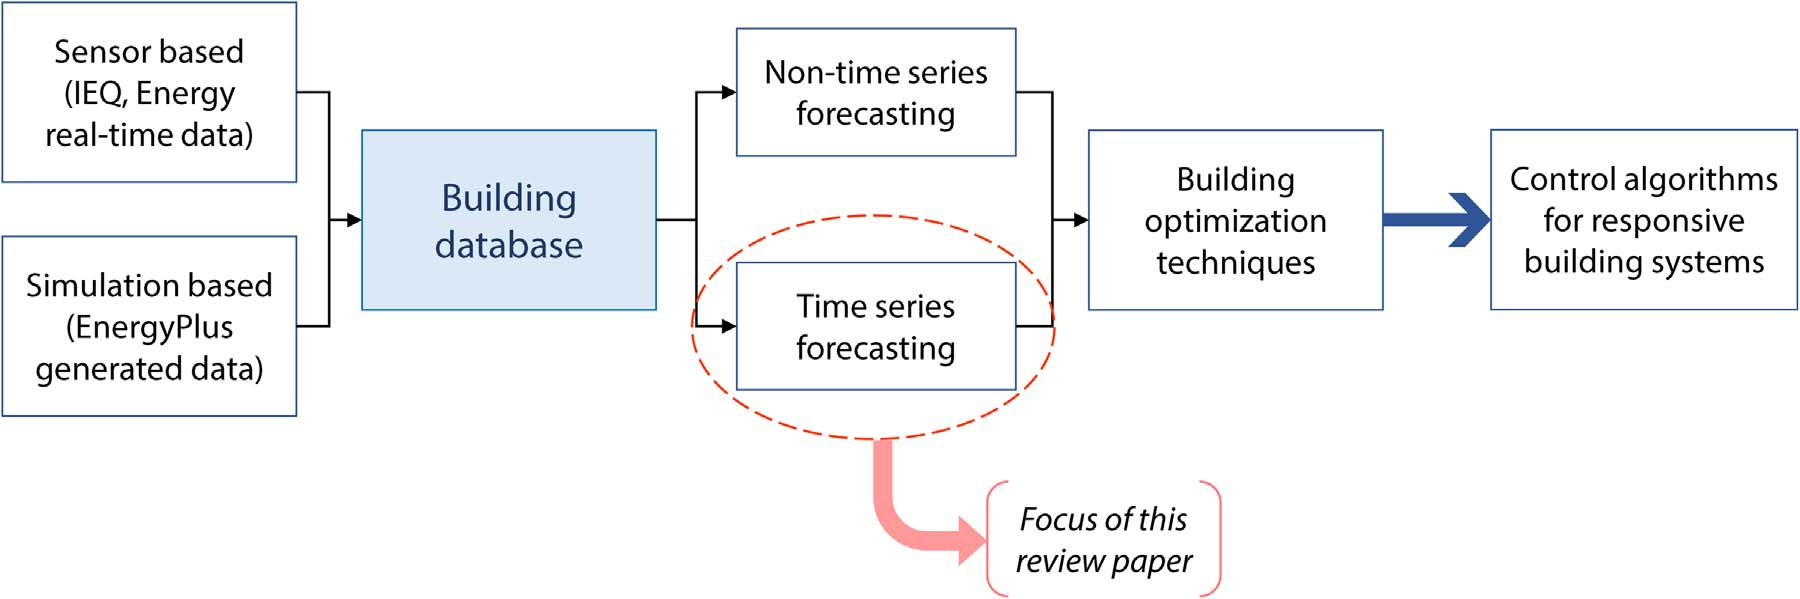
\includegraphics[width=14cm]{images/illustration.jpg}
%     \end{center}
%     \caption[‌اهمیت پیش‌بینی انرژی ساختمان‌ها برای بهینه سازی ساختمان‌ها]{تمرکز این گزارش نوشتاری در حوزه بهینه‌سازی ساختمان
%      \cite{DEB2017902}}
%     \label{fig:dc}
%     \end{figure}

% \noindent
% در فصل‌های بعدی نخست توضیحاتی در مورد پیش‌بینی مصرف انرژی ساختمان‌ها میدهیم و در مورد روش‌های تاریخی و قدیمی‌تر از 
% الگوریتم‌های هوش‌ مصنوعی صحبت خواهیم کرد که روش‌های مهندسی و آماری را شامل میشوند. در فصل ۳ الگوریتم‌های متنوع هوش مصنوعی برای پیش‌بینی سری داده‌های زمانی معرفی و به طور مفصل شرح داده میشوند و هر یک 
% معادلات مورد نیازشان توضیح داده میشود. در فصل ۴ معیار‌های سنجش بین این الگوریتم‌ها معرفی می‌شوند و آزمایش‌های متنوع 
% برای یافتن الگوریتم‌های مناسب را گزارش می‌دهیم و در نهایت در فصل ۵ با نتیجه‌گیری از مطالب گفته شده سعی در نتیجه‌گیری گزارش و ارائه پیشنهادات مناسب شده است.
\chapter{ یادگیری تقویتی}
\section{مقدمه}
به طور عمومی، یادگیری ماشین به دسته‌ای از الگوریتم‌ها و روش‌های محاسباتی گفته می‌شود که به ماشین‌ها امکان یادگیری از داده‌ها و تجربه‌های خود را می‌دهند.
یادگیری ماشین به دو دسته‌ی اصلی تقسیم می‌شود: یادگیری نظارت‌شده و یادگیری بدون نظارت.
در یادگیری نظارت‌شده، مدل به کمک داده‌های برچسب‌خورده آموزش داده می‌شود، و سپس برای پیش‌بینی خروجی‌های جدید از این مدل استفاده می‌شود.
در یادگیری بدون نظارت، مدل بدون داده‌های برچسب‌خورده آموزش داده می‌شود، و باید خودش مفاهیم و الگوهای موجود در داده‌ها را کشف کند.
یادگیری تقویتی در این دو دسته قرار نمی‌گیرد، و به عنوان یک دسته جداگانه در نظر گرفته می‌شود.

یادگیری تقویتی یک روش یادگیری ماشین است که به عامل اجازه می‌دهد تا رفتار بهینه را از طریق تعامل و آزمون و خطا با محیط یاد بگیرد.
در این روش، عامل مشاهدات خود را از محیط (به کمک سنسور)
دریافت کرده،
و بر اساس آن تصمیم خود را اخذ می‌کند.
پس از انجام هر عمل، محیط به عامل پاداشی می‌دهد که نشان‌دهنده‌ی عملکرد عامل در آن حالت است.
هدف این است که عامل مجموع پاداش‌های دریافتی خود را بیشینه کند، که در صورت صحیح بودن تعریف سیگنال پاداش، معمولا به معنای رسیدن به هدف مطلوب است.

یادگیری ماشین با سایر رویکرد‌های یادگیری ماشین مانند یادگیری نظارت‌شده و یادگیری بدون نظارت تفاوت‌های زیادی دارد، 
و معمولا بر مسائلی به کار می‌رود که تمرکز بر تصمیم‌گیری یا پیدا کردن سیاست بهینه بدون نیاز به داده‌های برچسب‌خورده است.
در عوض، عامل با اکتشاف و بهره‌برداری ابتدا انتقالات بین حالت‌ها و پاداش‌های مرتبط با آن‌ها را یاد می‌گیرد، و سپس سیاستی را یاد می‌گیرد که مجموع پاداش‌ها را بیشینه کند.


\section{اصول یادگیری تقویتی}
\subsection{عامل، محیط، حالت، عمل و پاداش}
در یادگیری تقویتی، عامل \LTRfootnote{Agent}
 تصمیم‌گیرنده برای رسیدن به هدف خود با محیط\LTRfootnote{Environment}
  تعامل دارد.
محیط معمولا به صورت مجموعه‌ای از حالت‌ها \LTRfootnote{State}
  و عمل‌هایی \LTRfootnote{Action}
    که عامل می‌تواند انجام دهد مدل می‌شود.
در هر گام، عامل مشاهده‌ای از حالت محیط را دریافت می‌کند و بر اساس آن تصمیمی اتخاذ می‌کند.
پس از انجام عمل، محیط به عامل پاداش \LTRfootnote{Reward}
  می‌دهد که نشان‌دهنده‌ی عملکرد عامل در آن حالت است.

\begin{figure}[H]
    \centering
    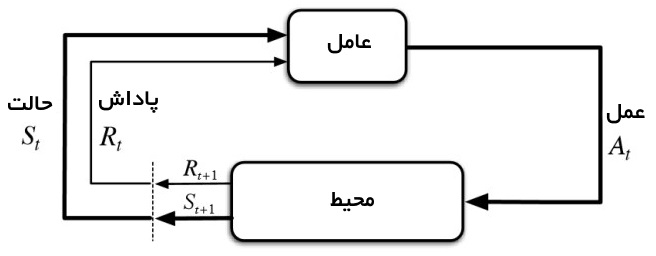
\includegraphics[width=0.75\textwidth]{images/agent_env.jpg}
    \caption{تعامل عامل و محیط}\label{fig:agent_env}

\end{figure}
% explain episodes here
در اکثر مواقع، یادگیری تقویتی در مسائلی استفاده می‌شود، که بتوان آن را به دنباله‌ای از گام‌ها تقسیم کرد که قطعا به یک حالت پایانی می‌رسد.
 هر یک از این دنباله‌ها را قسمت \LTRfootnote{Episode}
  می‌نامند.
\subsection{فرایند تصمیم‌گیری مارکوف}
فرایند تصمیم‌گیری مارکوف \LTRfootnote{Markov Decision Process (MDP)}
  مدلی است برای تصمیم‌گیری در محیط‌هایی که به صورت مارکوف هستند.
  محیط‌های دارای خاصیت مارکوف، محیط‌هایی هستند که حالت بعدی به صورت کامل به حالت فعلی و عمل انجام شده وابسته است.


  یک فرایند تصمیم‌گیری مارکوف، چهارتایی 
  $(S, A, P, R)$
  است که در آن:
  \begin{itemize}
      \item $S$ مجموعه‌ی تمام حالت‌های ممکن محیط است.
      \item $A$ مجموعه‌ی تمام عمل‌های ممکن است.
      \item $P$ تابع انتقال \LTRfootnote{Transition Function}
      است که به ازای هر حالت و عمل، توزیع احتمال حالت بعدی را مشخص می‌کند.
      \item $R$ تابع پاداش \LTRfootnote{Reward Function}
      است که به ازای هر حالت و عمل، پاداش مورد انتظار را مشخص می‌کند.
      \item فاکتور تخفیف $\gamma$ نیز معمولا به عنوان یک پارامتر دیگر در نظر گرفته می‌شود که نشان‌دهنده‌ی اهمیت پاداش‌های آینده نسبت به پاداش‌های فعلی است.
  \end{itemize}
همانطور که گفته شد، در هر گام عامل با اخذ تصمیم خود، محیط را به حالت جدیدی می‌برد و پاداشی دریافت می‌کند.
به مجموع کل پاداش‌هایی که عامل در یک قسمت دریافت می‌کند، خروجی \LTRfootnote{Return}
 گفته می‌شود.
 \begin{equation}\label{eq:return}
     G_t = R_{t+1} + \gamma \times R_{t+2} + \gamma^2 \times R_{t+3} + \cdots = \sum_{k=0}^\infty \gamma^k \times R_{t+k+1}
 \end{equation}
\subsection{سیاست، تابع ارزش، و تابع ارزش عمل}
سیاست \LTRfootnote{Policy}
یک تابع از حالت‌ها به عمل‌ها است که نشان‌دهنده‌ی رفتار عامل در هر حالت محیط است.
در واقع مسئله یادگیری تقویتی را می‌توان به ((یافتن سیاستی که مجموع پاداش‌ها را بیشینه می‌کند)) تعبیر کرد.
\begin{equation}\label{eq:policy}
    \pi(a|s) = \mathbb{P}\{A_t = a | S_t = s\}
\end{equation}

تابع ارزش \LTRfootnote{Value Function} $V(s)$
یک تابع از حالت‌ها است که نشان‌دهنده‌ی میزان پاداش مورد انتظار از یک حالت تا به انتهای قسمت است.
\begin{equation}\label{eq:value_function}
    v_\pi(s) = \mathbb{E}_\pi\{G_t | S_t = s\} = \sum_{a \in A}\pi(a|s)\times\{R_s^a + \gamma \times \sum_{s' \in S}p(s'|s,a)\times v_\pi(s')\}
\end{equation}
تابع ارزش عمل \LTRfootnote{Action Value Function} $Q(s, a)$
نیز مشابه تابع ارزش است، با این تفاوت که به جای حالت، از یک حالت و یک عمل مشخص محاسبه می‌شود. رایج است که به این تابع، تابع کیو گفته شود.
\begin{equation}\label{eq:q_function}
    q_\pi(s,a) = \mathbb{E}_\pi\{G_t | S_t = s, A_t = a\} = R_s^a + \gamma \times \sum_{s' \in S}p(s'|s,a)\times v_\pi(s')
\end{equation}
به این معادلات، که از کلیدی‌ترین روابط در یادگیری تقویتی هستند، معادله بلمن \LTRfootnote{Bellman Equation} گفته می‌شود.
\section{الگوریتم‌های پایه یادگیری تقویتی}
\subsection{برنامه‌نویسی پویا}
همان‌طور که در معادله \ref{eq:value_function} مشخص است، می‌توان تابع ارزش را به صورت بازگشتی محاسبه کرد.
این روش برنامه‌نویسی پویا \LTRfootnote{Dynamic Programming}
نام دارد.
\subsubsection{یادگیری به کمک تکرار ارزش}
در روش تکرار ارزش \LTRfootnote{Value Iteration}،
، ابتدا تابع ارزش را به صورت تصادفی مقداردهی می‌کنیم و سپس آن را به صورت بازگشتی به روزرسانی می‌کنیم.
قابل اثبات است که این روش به تابع ارزش بهینه همگرا می‌شود.
به صورت شهودی نیز، می‌توان دید که ارزش از سمت حالت‌های پایانی به سمت حالت‌های ابتدایی به روزرسانی می‌شود.
\subsubsection{یادگیری به کمک تکرار سیاست}
در روش تکرار سیاست \LTRfootnote{Policy Iteration}،
ابتدا سیاست را به صورت تصادفی مقداردهی می‌کنیم و سپس تابع ارزش را برای آن محاسبه می‌کنیم.
سپس سیاست را به صورت بازگشتی به روزرسانی می‌کنیم. 
این فرآیند را تا زمانی که سیاست تغییر نکند ادامه می‌دهیم.
قابل اثبات است که این روش به سیاست بهینه همگرا می‌شود.

در عمل، با توجه به اینکه معمولا به تابع انتقال دسترسی نداریم، نمی‌توانیم از روش‌های برنامه‌نویسی پویا به صورت مستقیم استفاده کنیم.
در واقع نیاز به راه حل‌های مستقل از مدل داریم که به کمک نمونه‌برداری و کاوش محیط، سیاست بهینه را یاد بگیرند.

\subsection{یادگیری به کمک نمونه‌برداری مونته کارلو}
در روش‌های یادگیری به کمک نمونه‌برداری مونته کارلو \LTRfootnote{Monte Carlo Sampling}،
به جای استفاده از مدل، از نمونه‌برداری برای تخمین ارزش استفاده می‌شود.
کافی‌ست ابتدا یک قسمت را به طور کامل اجرا کنیم، و سپس ارزش هر حالت را، به سمت خروجی قسمت، به روزرسانی کنیم:
\begin{equation}\label{eq:mc_q_function}
    Q(s_t, a_t) = Q(s_t, a_t) + \alpha \times (G_t - Q(s_t, a_t))
\end{equation}
که در این فرمول، $\alpha$
نرخ یادگیری \LTRfootnote{Learning Rate} است.

لازم به ذکر است که در حین اجرای قسمت، از سیاست اپسیلون-حریصانه \LTRfootnote{$\epsilon$-greedy} استفاده می‌شود.
در این سیاست، با احتمال $\epsilon$ عملی تصادفی انجام می‌شود و با احتمال $1-\epsilon$ عملی که ارزش بیشتری دارد انجام می‌شود.
دلیل استفاده از این سیاست، نیاز به کاوش محیط و جلوگیری از گیر کردن در حالت‌های محلی است.

از معایب این روش، می‌توان به نیاز به اجرای کامل قسمت‌ها و نیاز به زمان برای یادگیری اشاره کرد. به همین دلیل، این روش برای مسائلی که قسمت‌های طولانی دارند، مناسب نیست.
از مشکلات دیگر این روش، عدم استفاده از ویژگی مارکوف محیط است.
\subsection{یادگیری به کمک تفاوت زمانی}
همان‌طور که گفته شد، استفاده از یادگیری مونته‌کارلو باعث می‌شود که عامل در حین انجام قسمت، از تجربه‌ی قبلی خود استفاده نکند
و به روز رسانی ارزش‌ها فقط پس از اتمام قسمت انجام شود. به این روش، یادگیری آفلاین \LTRfootnote{Offline Learning} گفته می‌شود.
در روش یادگیری به کمک تفاوت زمانی \LTRfootnote{Temporal Difference Learning}،
عامل در حین انجام قسمت، از تجربه‌ی خود استفاده می‌کند و ارزش‌ها را به صورت آنلاین به روزرسانی می‌کند.
در واقع به کمک معادله بلمن، مقادیر کیو به سمت مقدار کیو بعدی به روزرسانی می‌شوند.

پیاده‌سازی این دو الگوریتم، به دو روش دید رو به جلو و دید رو به عقب انجام می‌شود.
در حالت دید رو به جلو، مشابه با یادگیری مونته کارلو، پس از رسیدن به پایان قسمت، ارزش‌ها به روزرسانی می‌شوند.
در حالت دید رو به عقب، ارزش‌ها به صورت آنلاین به روزرسانی می‌شوند. به این صورت که پس از دریافت یک پاداش، عامل مقادیر کیو $n$ حالت‌ قبلی خود را به روزرسانی می‌کند.
\subsubsection{تی‌دی صفر}
در ساده‌ترین حالت، عامل در حین انجام عمل، با دیدن یک گام در آینده یا گذشته، ارزش عمل فعلی را به روزرسانی می‌کند.
به این روش تی‌دی صفر \LTRfootnote{TD(0)} گفته می‌شود.
\begin{equation}\label{eq:td_zero_q_function}
    Q(s_t, a_t) = Q(s_t, a_t) + \alpha \times (R_{t+1} + \gamma \times Q(s_{t+1}, a_{t+1}) - Q(s_t, a_t))
\end{equation}
در واقع، به کمک رابطه بلمن
(که فرم ارزش عمل آن در رابطه  \ref{eq:q_function} دیده می‌شود)
میزان صحیح بودن ارزش عمل فعلی، با ارزش عمل بعدی و پاداش فعلی مقایسه می‌شود و ارزش عمل فعلی به روزرسانی می‌شود.
\subsubsection{ تی‌دی لامبدا رو به جلو}
در روش تی‌دی $\lambda$،
\LTRfootnote{TD($\lambda$)}
با دید رو به جلو
به جای استفاده از یک گام در آینده ، از یک ترکیب خطی از پاداش‌ها و بازگشت چندین گام استفاده می‌شود.
به این ترکیب خطی، $\lambda$-بازگشت \LTRfootnote{$\lambda$-return} گفته می‌شود.
\begin{equation}\label{eq:td_lambda_q_function}
    Q(s_t, a_t) = Q(s_t, a_t) + \alpha \times (G_t^\lambda - Q(s_t, a_t))
\end{equation}
که در این رابطه، $G_t^\lambda$
به صورت زیر محاسبه می‌شود:
\begin{equation}\label{eq:td_lambda_return}
    G_t^\lambda = (1-\lambda)\times\sum_{n=1}^\infty \lambda^{n-1} \times G_t^{(n)}
\end{equation}
که در آن $G_t^{(n)}$، 
مقدار بازگشتی بعد از $n$ گام است،
و $\lambda$
یک پارامتر بین صفر و یک است که نشان‌دهنده‌ی اهمیت پاداش‌های آینده نسبت به پاداش‌های فعلی است.
می‌توان میزان اهمیت پاداش‌های را به ازای مقادیر مختلف $\lambda$ مشاهده کرد.
\begin{figure}[H]
    \centering
    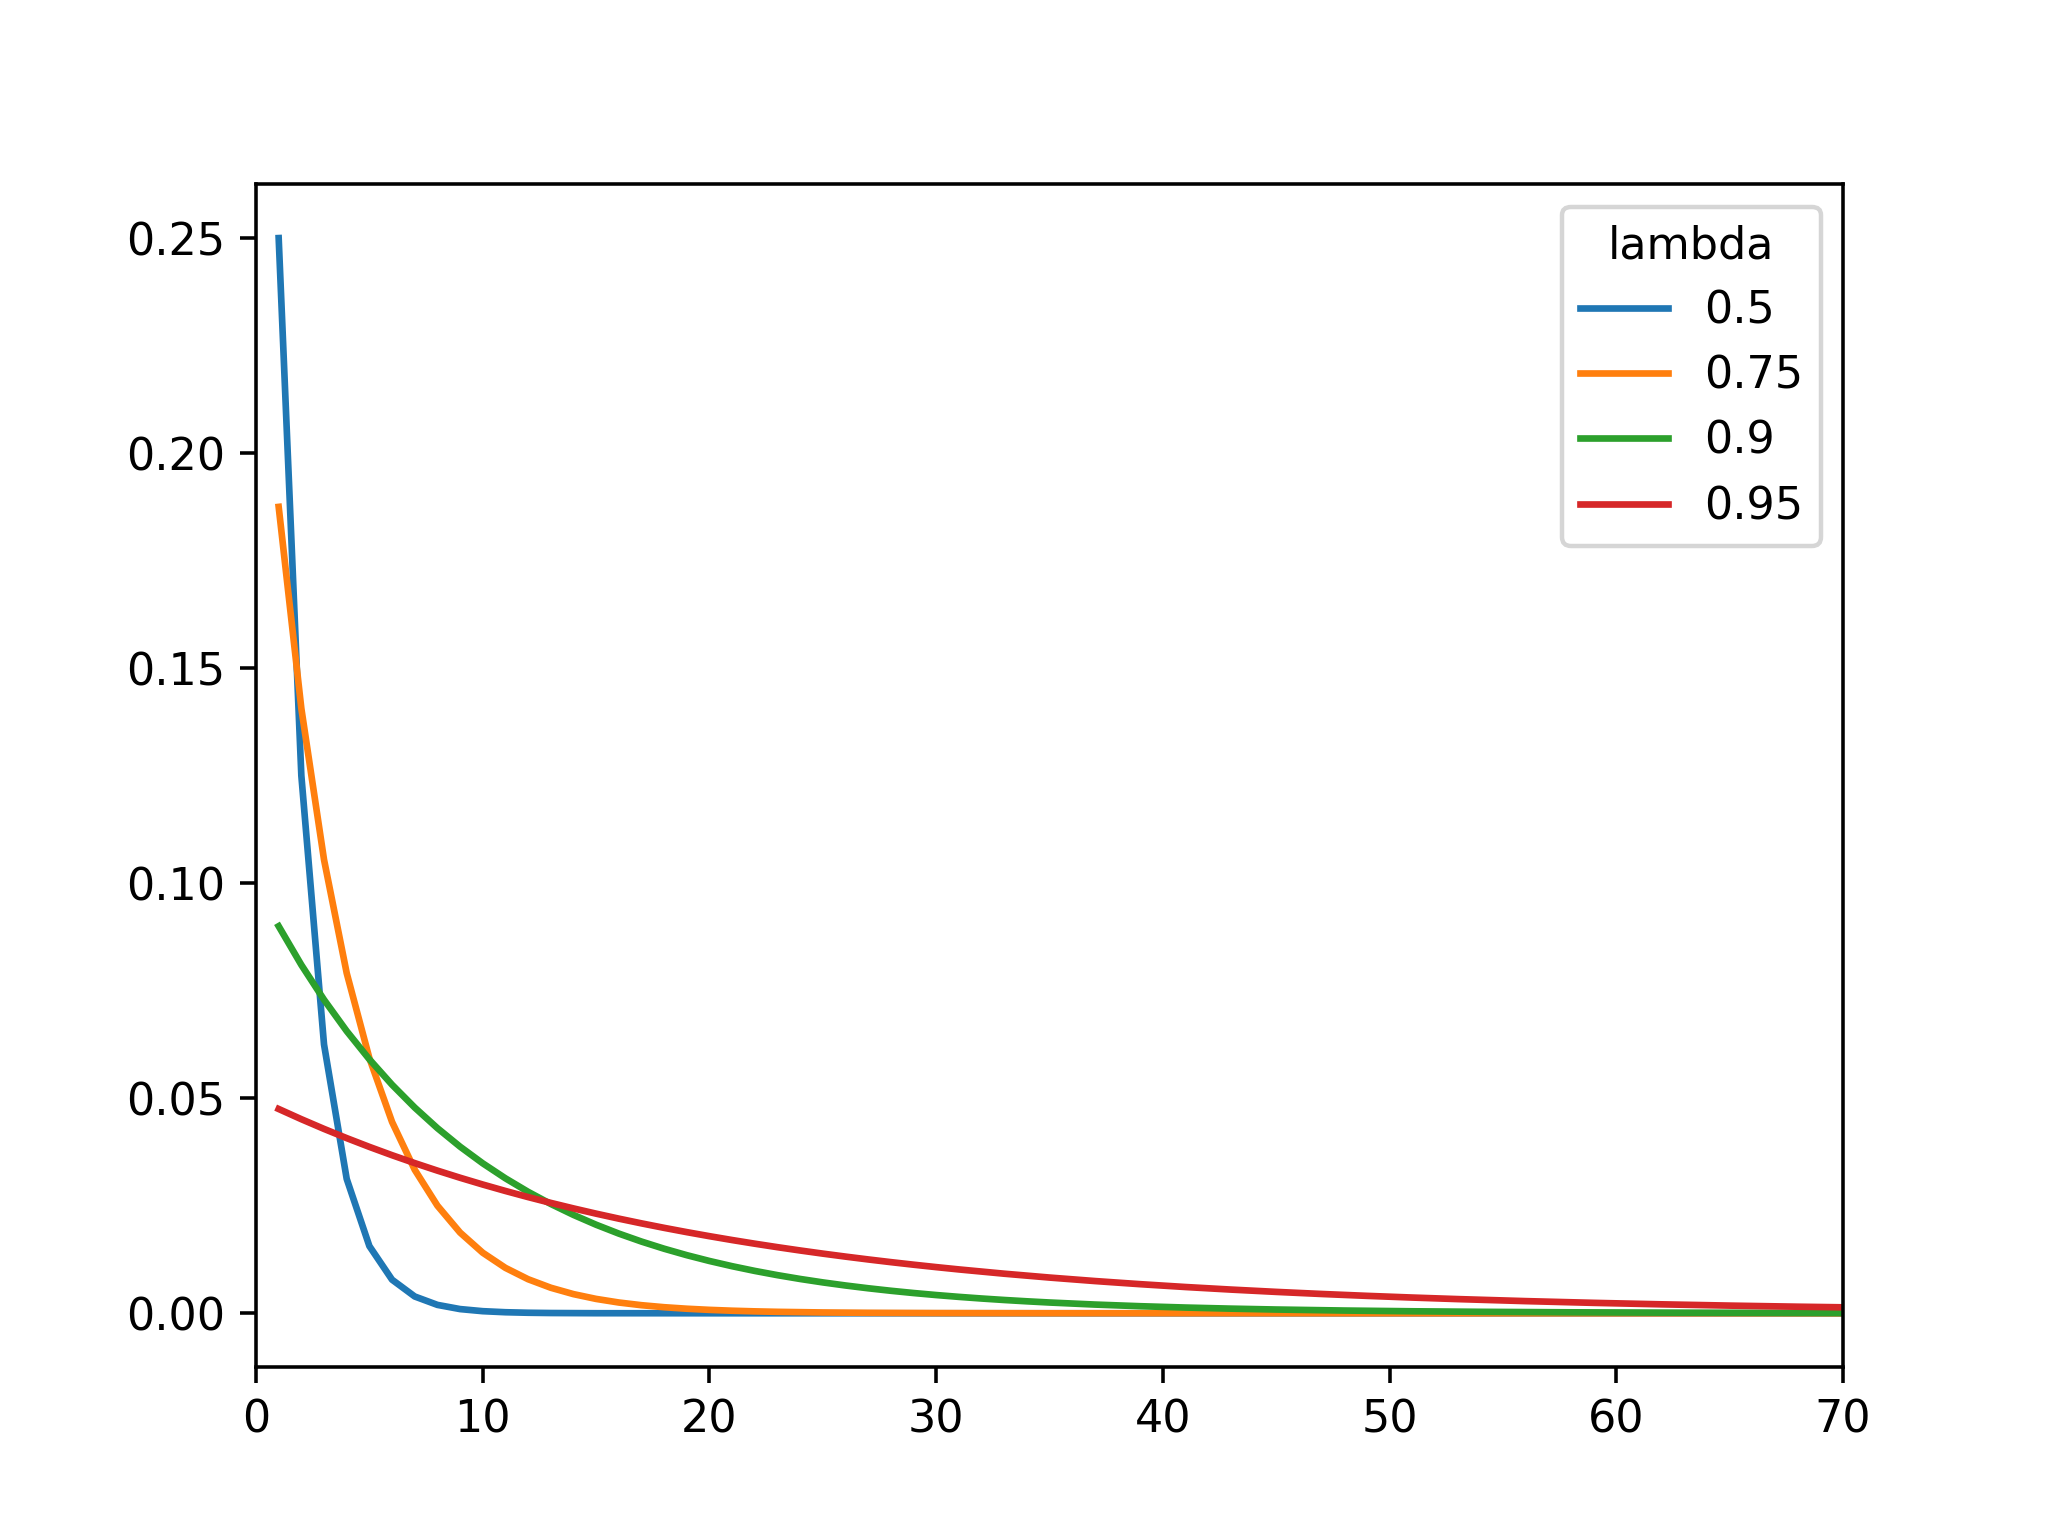
\includegraphics[width=0.75\textwidth]{images/lambda_return_weight.png}
    \caption{تاثیر پارامتر  $\lambda$ بر اهمیت پاداش‌های آینده. 
    محور افقی نماینده تعداد گام‌ها، و محور عمودی نماینده وزن این بازگشت متناظر با آن است.}\label{fig:td_lambda}
    
\end{figure}
\subsubsection{تی‌دی لامبدا رو به عقب}
در روش تی‌دی $\lambda$ با دید رو به عقب،
از مفهومی به نام آثار شایستگی \LTRfootnote{Eligibility Traces} استفاده می‌شود.
این مفهوم، نشان‌دهنده‌ی این است که هر عملی که در گذشته انجام شده و موجب تغییر ارزش عملی شده است،  به چه میزان روی این تغییر سهیم بوده‌است.

ابتدا به ازای هر حالت و عمل، یک متغیر آثار شایستگی $E(s, a)$
صفر تعیین می‌شود و سپس در هر گام، این متغیر به صورت زیر به روزرسانی می‌شود:
\begin{equation}\label{eq:eligibility_trace}
    E(s, a) = \gamma \times \lambda \times E(s, a) + 1(s = s_t, a = a_t)
\end{equation}
در واقع کل آثار شایستگی در لامبدا ضرب شده، و یکی به آثار شایستگی عمل و حالت فعلی اضافه می‌شود.
در این حالت، آثار شایستگی معادل با میزان نزدیکی زمانی هر حالت و عمل، به حالت و عمل فعلی است.

سپس ارزش عمل به صورت زیر به روزرسانی می‌شود:
\begin{equation}\label{eq:td_lambda_backward_q_function}
    Q(s, a) = Q(s, a) + \alpha \times \delta \times E(s, a)
\end{equation}
که در این رابطه، $\delta$
خطای تخمین است که به صورت زیر محاسبه می‌شود:
\begin{equation}\label{eq:td_lambda_backward_delta}
    \delta = R_{t+1} + \gamma \times (Q(s_{t+1}, a_{t+1}) - Q(s_t, a_t))
\end{equation}
می‌توان نشان داد که پس از انجام یک قسمت، به‌روز‌رسانی‌های انجام شده توسط این روش، معادل با به‌روز‌رسانی‌های انجام شده توسط تی‌دی $\lambda$ با دید رو به جلو است.

با ترکیب این روش و سیاست اپسیلون-حریصانه، می‌توان به یک روش یادگیری تقویتی کارا دست یافت که 
سارسا-لامبدا \LTRfootnote{SARSA($\lambda$)} نام دارد.
\section{استفاده از تقریب‌گر تابع}
با توجه به زیاد بودن تعداد حالت‌های ممکن در اکثر مسائل، یادگیری با روش‌های توضیح‌داده‌شده بسیار کند و حتی غیرمعقول می‌باشد.
از این رو، به جای نگه‌داری مقادیر \lr{Q} 
در یک جدول به ازای هر زوج حالت-عمل
 از تقریب‌گر‌های تابع\LTRfootnote{Function Approximators}
  برای تخمین این مقادیر استفاده می‌کنیم.

    از تقریب‌گر‌های تابع مختلفی می‌توان برای این کار استفاده کرد.
    از جمله‌ی این تقریب‌گر‌ها می‌توان به شبکه‌های عصبی، درخت‌های تصمیم، و توابع پایه‌ای مثل چندجمله‌ای‌ها اشاره کرد.

    در واقع ابتدا از حالت، برخی ویژگی‌های مهم را استخراج کرده، سپس از این ویژگی‌ها برای تخمین ارزش‌ها به کمک پارامتر‌هایی که قرار است یاد گرفته شوند استفاده می‌کنیم.
    رایج است که در روابط، به این پارامتر‌ها با 
    $\theta$ یا $w$
    اشاره شود.

\begin{figure}[H]
    \centering
    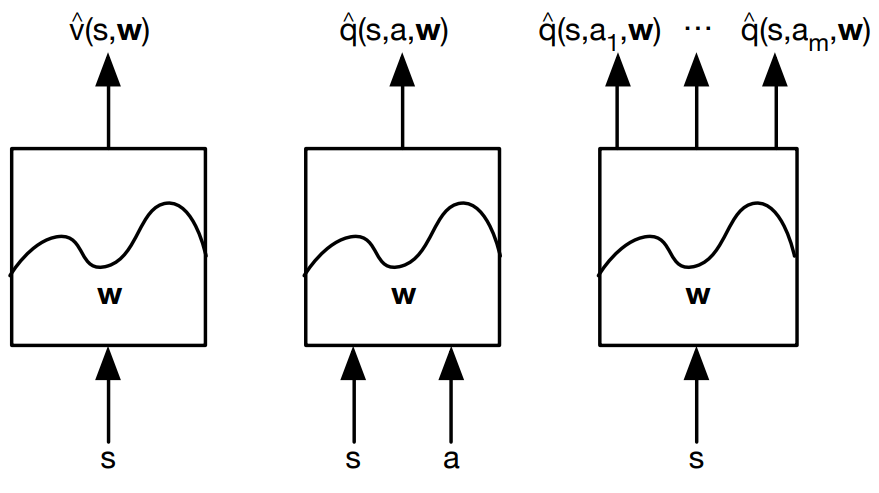
\includegraphics[width=0.75\textwidth]{images/function_approximators.png}
    \caption{روش‌های مختلف استفاده از تقریب‌گر تابع}\label{fig:func_approx}
\end{figure}
حال کافی‌ست که معادلات \ref{eq:td_zero_q_function}، \ref{eq:td_lambda_q_function}، و \ref{eq:td_lambda_backward_q_function} را به صورت تقریبی برای تقریب‌گر تابع بنویسیم،
و به‌جای به روزرسانی مقادیر \lr{Q}، پارامتر‌های تقریب‌گر تابع را به‌روز کنیم.
با توجه به نیاز به به‌روز‌رسانی، لازم است از تقریب‌گر‌های مشتق‌پذیر استفاده کنیم.
همانطور که در عکس \ref{fig:func_approx}
می‌توان دید، در حالتی که از تقریب‌گر‌های تابع برای پیش‌بینی مقادیر \lr{Q} استفاده می‌شود،
رایج است از عبارت 
$Q(s, a; \theta)$
یا $Q(s, a; w)$
برای نشان دادن این تقریب‌گر‌ها استفاده کرد.

\section{الگوریتم یادگیری \lr{Q} عمیق}
این الگوریتم، یکی از مستقیم‌ترین راه‌های استفاده از تقریب‌گر‌های توابع، برای ترکیب یادگیری عمیق و تقویتی است.
در این الگوریتم، هدف این است که مشابه با حالت سوم شکل \ref{fig:func_approx}،
پارامتر‌های یک شبکه عصبی را به‌گونه‌ای تنظیم کنیم که مقادیر ارزش-عمل را بتواند تخمین بزند.
از دستاورد‌های این الگوریتم، عملکرد در حد انسان در چندین بازی آتاری \LTRfootnote{Atari} است
که توسط تیم دیپ‌مایند \LTRfootnote{DeepMind}
در سال ۲۰۱۵ به‌وقوع پیوست.

شبکه‌های عصبی الهام گرفته از ساختار و عملکرد مغز انسان هستند که برای یادگیری از داده‌ها و تصمیم‌گیری‌های پیچیده استفاده می‌شوند.
 این شبکه‌ها از واحدهای پردازشی به نام پرسپترون‌ها تشکیل شده‌اند که در لایه‌های مختلف قرار گرفته‌اند و از طریق وزن‌هایی به هم متصل می‌شوند.
 
 یادگیری در شبکه‌های عصبی اغلب از طریق فرایندی به نام نزول گرادیان انجام می‌گیرد که در آن وزن‌های شبکه به صورت تکراری تنظیم می‌شوند تا خطا بین پیش‌بینی‌های شبکه و داده‌های واقعی به حداقل برسد. این فرایند شامل محاسبه گرادیان یا شیب تابع خطا نسبت به وزن‌ها و به‌روزرسانی وزن‌ها در جهت مخالف گرادیان برای کاهش خطا است.
% formula for gradient descent
\begin{equation}\label{eq:gradient_descent}
    \theta_{t+1} = \theta_t - \alpha \nabla J(\theta_t)
\end{equation}
در این فرمول، $\theta$
پارامتر‌های شبکه،
\lr{$\alpha$}
نرخ یادگیری،
\lr{$J$}
تابع خطا، و
\lr{$\nabla J$}
گرادیان تابع خطا نسبت به پارامتر‌ها هستند.

برای اینکه یادگیری شبکه عصبی با ثبات بالاتری رخ دهد، این الگوریتم از دو تکنیک 
\textbf{بازیابی تجربه}
و
\textbf{استفاده از شبکه هدف}
بهره می‌برد.
\subsection{بازیابی تجربه}
برای رفع مشکلات داده‌های همبسته و توزیع‌های غیر ایستا در یادگیری آنلاین، \lr{DQN} از یک مکانیزم بازیابی تجربه استفاده می‌کند. این شامل ذخیره تجربیات عامل در هر گام زمانی در یک بافر بازیابی و سپس نمونه‌برداری تصادفی ریزدسته‌ها \LTRfootnote{Mini-batches}
 از این بافر برای آموزش شبکه است. این رویکرد به شکستن همبستگی بین نمونه‌های پیاپی کمک می‌کند و فرآیند یادگیری را پایدار می‌سازد.
\subsection{استفاده از شبکه هدف}
\lr{DQN} یک شبکه دوم به نام شبکه هدف را برای استقرار بیشتر آموزش معرفی می‌کند. شبکه هدف یک کپی از شبکه \lr{Q} است، اما وزن‌های آن کمتر به‌روز می‌شوند. این جداسازی نوسان ارزش‌های هدف در به‌روزرسانی یادگیری \lr{Q} را کاهش می‌دهد و خطر حلقه‌های بازخورد خودتقویتی را کاهش می‌دهد.
\subsection{فرآیند یادگیری}
در ابتدا وزن‌های شبکه ارزش-عمل را به صورت تصادفی تنظیم می‌کنیم و آن را $\theta$ می‌نامیم.
 شبکه هدف را با وزن‌های یکسان مقداردهی می‌کنیم و آن را $\theta^-$ می‌نامیم.
و بافر بازیابی را
به طول $N$ که یک ابرپارامتر است، مقداردهی می‌کنیم.

سپس در هر حالت، پاداش‌های خروجی شبکه اصلی را می‌گیریم و به صورت اپسیلون-حریصانه عمل را انتخاب می‌کنیم؛
یعنی به احتمال $\epsilon$ رفتار تصادفی داریم، 
و با احتمال $1-\epsilon$
رفتار با بالاترین ارزش-عمل پیش‌بینی شده را برمیداریم، یعنی: $a_t = \underset{a}{\mathrm{argmax}} Q(s_t, a; \theta)$.
ترکیب چهارتایی حالت قبل عمل، عمل انتخاب شده، پاداش دریافتی، و حالت بعد عمل $(s_t,a_t,r_t,s_{t+1})$
را به بافر اضافه می‌کنیم.
یک گروه با اندازه مشخص را با نمونه‌برداری تصادفی از بافر انتخاب می‌کنیم، و به صورت زیر یادگیری را انجام می‌دهیم:
\begin{equation}\label{dqn_label}
    y_j = \begin{cases}
        r_j & \text{اگر $s_{j+1}$ حالت پایانی قسمت باشد} \\
        r_j + \gamma \times \max_{a'} Q(s_{j+1}, a'; \theta^-) & \text{در غیر این صورت}
    \end{cases}
\end{equation}
در این معادله $y_j$ تخمینی از میزان پاداش دریافتی واقعی است، که مشابه با روش‌های \lr{TD}، از ترکیب پاداش دریافتی و ارزش-عمل بعدی به دست می‌آید.
بنابرین می‌توان از این مقدار، مشابه با برچسب در یادگیری نظارت‌شده، برای آموزش شبکه استفاده کرد.
میزان خطای شبکه به صورت زیر تعریف می‌شود:
\begin{equation}\label{dqn_loss}
    L(\theta) = \mathbb{E}[(y_j - Q(s_j, a_j; \theta))^2]
\end{equation}
که با استفاده از این خطا، می‌توان گرادیان تابع خطا نسبت به وزن‌های شبکه را به دست آورد و
با استفاده از این گرادیان، می‌توان وزن‌های شبکه را به‌روز کرد:
\begin{equation}\label{dqn_update}
    \theta_{t+1} = \theta_t - \alpha \nabla_\theta L(\theta)
\end{equation}
در نهایت کافی‌ست به صورت تناوبی و هر چند گام یک بار وزن‌های شبکه هدف را برابر با کپی وزن‌های شبکه اصلی قرار دهیم. با تکرار این مراحل، به شبکه عصبیی دست می‌یابیم که قدرت پیش‌بینی ارزش‌های عمل را دارد.


حال می‌توان اهمیت دو تکنیک گفته شده را بهتر فهمید: در صورت عدم استفاده از شبکه هدف، باید همزمان از شبکه اصلی برای پیش‌بینی آینده (در فرمول \ref{dqn_label}) و انتخاب عمل استفاده کنیم، که می‌تواند به مشکلاتی مانند نوسانات در آموزش و حلقه‌های بازخورد خودتقویتی منجر شود.
همچنین در صورت عدم استفاده از بافر تجربه، باید صرفا از تجارب اخیر خود استفاده کنیم، که در این صورت هبستگی بین نمونه‌ها و توزیع‌های غیر ایستا می‌تواند مشکل‌ساز شود.
\section{الگوریتم بهبود گرادیان سیاست معین عمیق}
الگوریتم بهبود گرادیان سیاست معین عمیق \LTRfootnote{Deep Deterministic Policy Gradient} یا به اختصار \lr{DDPG}، یک الگوریتم یادگیری تقویتی است که برای حل مسائل پیوسته و فضای عمل پیوسته طراحی شده است.
همانطور که در بخش‌های قبل دیدیم، برای انتخاب عمل معمولا از سیاست اپسیلون-حریصانه استفاده می‌شود، اما این روش برای فضای عمل پیوسته مناسب نیست، چرا که به‌دست‌آوردن بیشینه در فضای پیوسته به مراتب دشوار‌تر از حالت گسسته است.
این الگوریتم از نوع یادگیری خارج از سیاست است؛ به این معنا که عامل با دنبال کردن سیاستی که سیاست انتخابی خود نیست به بهبود عملکرد خود می‌پردازد.

\lr{DDPG}
از دو شبکه عصبی استفاده می‌کند: یک شبکه برای تخمین ارزش عمل که به آن نقاد می‌گوییم، و یک شبکه برای تخمین سیاست و انتخاب عمل که به آن بازیگر می‌گوییم.
شبکه نقاد مشابه با شبکه
 \lr{Q}
  در 
  \lr{DQN}
   است، با این تفاوت که حالت و عمل را ورودی گرفته و ارزش عمل را خروجی می‌دهد.
 و شبکه سیاست یک شبکه عصبی است که خروجی آن عمل است.
 این الگوریتم مشابه با \lr{DQN}
 از بافر تجربه برای ذخیره تجربیات عامل، و از شبکه‌های هدف برای هر دو شبکه نقاد و بازیگر استفاده می‌کند.
 البته در این الگوریتم، به‌جای کپی وزن‌های شبکه به شبکه هدف، از میانگین وزن‌دار استفاده می‌شود تا به روز‌رسانی آرام‌تر انجام شود و ثبات بیشتری داشته باشد.
 \begin{figure}[H]
    \centering
    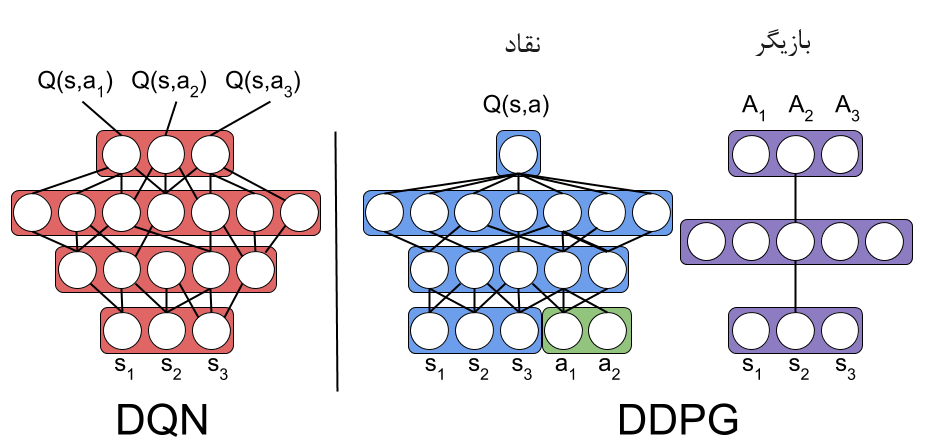
\includegraphics[width=0.85\textwidth]{images/actor_critic.png}
    \caption{شبکه‌های عصبی بازیگر و نقاد در الگوریتم \lr{DDPG} و مقایسه با \lr{DQN}}\label{fig:actor_critic}
\end{figure}
رایج است که شبکه ارزش عمل را با $Q(s, a; \phi)$ و شبکه سیاست را با $\mu(s; \theta)$ نشان دهیم.
فرآیند یادگیری این الگوریتم به صورت زیر است:
\begin{enumerate}
    \item ابتدا وزن‌های شبکه‌های نقاد و بازیگر را به صورت تصادفی مقداردهی می‌کنیم و آن‌ها را به ترتیب $\phi$ و $\theta$ می‌نامیم.
    \item بافر تجربه را به طول $N$ مقداردهی می‌کنیم.
    \item در هر گام زمانی، حالت را به شبکه بازیگر می‌دهیم و عملی که این شبکه پیشنهاد می‌دهد را انجام می‌دهیم.
    \item پاداش دریافتی و حالت بعد عمل را به بافر تجربه اضافه می‌کنیم.
    \item یک ریزدسته از بافر تجربه را انتخاب کرده و با استفاده از فرمول زیر، مقدار واقعی ارزش حالت را (طبق الگوریتم \lr{TD}) محاسبه می‌کنیم:
    \begin{equation}\label{ddpg_label}
        y_j = \begin{cases}
            r_j & \text{اگر $s_{j+1}$ حالت پایانی قسمت باشد} \\
            r_j + \gamma \times Q(s_{j+1}, \mu(s_{j+1}; \theta^-); \phi^-) & \text{در غیر این صورت}
        \end{cases}
    \end{equation}
    \item خطای شبکه نقاد را به صورت زیر محاسبه می‌کنیم:
    \begin{equation}\label{ddpg_critic_loss}
        L(\phi) = \mathbb{E}[(y_j - Q(s_j, a_j; \phi))^2]
    \end{equation}
    و وزن‌های شبکه نقاد را به‌روز می‌کنیم:
    \begin{equation}\label{ddpg_critic_update}
        \phi_{t+1} = \phi_t - \alpha \nabla_\phi L(\phi)
    \end{equation}
    \item خطای شبکه بازیگر را به صورت زیر محاسبه می‌کنیم:
    \begin{equation}\label{ddpg_actor_loss}
        L(\theta) = -\mathbb{E}[Q(s, \mu(s; \theta); \phi)]
    \end{equation}
    و وزن‌های شبکه بازیگر را به‌روز می‌کنیم:
    \begin{equation}\label{ddpg_actor_update}
        \theta_{t+1} = \theta_t + \alpha \nabla_\theta L(\theta)
    \end{equation}
    \item در نهایت هر چند گام یک بار، وزن‌های شبکه‌های هدف را به‌روز می‌کنیم:
    \begin{equation}\label{ddpg_target_actor_update}
        \theta^-_{t+1} = \tau \theta_t + (1-\tau) \theta^-_t
    \end{equation}
    \begin{equation}\label{ddpg_target_critic_update}
        \phi^-_{t+1} = \tau \phi_t + (1-\tau) \phi^-_t
    \end{equation}
\end{enumerate}
همانطور که مشاهده‌شد، این الگوریتم تعداد زیادی پارامتر دارد که باید به‌درستی تنظیم شوند تا به عملکرد بهینه برسد.
از جمله این پارامتر‌ها می‌توان به نرخ یادگیری ($\alpha$ که می‌تواند برای شبکه‌های نقاد و بازیگر متفاوت باشد)،
، نرخ تخفیف ($\gamma$)،
فرکانس به‌روزرسانی شبکه‌ها (هر چند گام یک بار ریزدسته انتخاب می‌کنیم و مراحل ۵ تا ۸ را طی می‌کنیم)،
فرکانس به‌روزرسانی وزن‌های هدف (هر چند گام یک بار وزن‌های شبکه‌های هدف را به‌روزرسانی می‌کنیم)
 ، اندازه ریزدسته، طول بافر تجربه، و ضریب به‌روزرسانی شبکه‌های هدف $\tau$
  اشاره کرد.
\section{جمع‌بندی}

% پیش‌بینی داده‌های سری زمانی از زمان گذشته مورد توجه محققین و متخصصین بوده است. در نتیجه در گذر زمان روش‌های متنوعی برای این موضوع پیشنهاد شده‌اند.
% .آمار و احتمالات از علوم بسیار قدیمی بشریت محسوب میشود یکی از روش‌های قدیمی برای پیش‌بینی داده‌های سری زمانی میباشد در کنار این روش، روش‌های مهندسی نیز در دهه‌های گذشته استفاده شده‌اند.
% در این فصل برای ارائه‌ی یک دید جامع و مناسب در مورد پیش‌بینی مصرف انرژی ساختمان‌ها در مورد هر دو روش گفته شده صحبت میکنیم و در نهایت در مورد روش‌های هوش‌مصنوعی توضیحاتی را ارائه میکنیم.


% \section{روش آماری}

% مدل‌های رگرسیون آماری صرفا مصرف انرژی یا شاخص انرژی را با متغیرهای تأثیرگذار مرتبط می‌کنند. این مدل‌های تجربی از داده‌های عملکرد تاریخی ایجاد شده‌اند، به این معنی که قبل از آموزش مدل‌ها، باید داده‌های تاریخی کافی را جمع‌آوری کنیم. تحقیقات زیادی بر روی مدل های رگرسیون در مورد مسائل زیر انجام شده است. اولین مورد پیش بینی مصرف انرژی بر روی متغیرهای ساده شده مانند یک یا چند پارامتر آب و هوا است. مورد دوم پیش بینی برخی از شاخص انرژی مفید است. مورد سوم، تخمین پارامترهای مهم مصرف انرژی، مانند ضریب تلفات حرارتی کل، ظرفیت حرارتی کل و ضریب افزایش است که در تحلیل رفتار حرارتی ساختمان یا سیستم‌های سطح فرعی مفید هستند.
% \\
% در برخی از مدل‌های مهندسی ساده‌شده، از رگرسیون برای ارتباط مصرف انرژی با متغیرهای آب و هوایی برای به دست آوردن امضای انرژی استفاده می‌شود \cite{pfafferott2005thermal,bauer1998simplified}. بائر\LTRfootnote{Bauer} و اسکارتزینی\LTRfootnote{Scartezzini} \cite{bauer1998simplified} یک روش رگرسیون را برای انجام محاسبات گرمایش و سرمایش به طور همزمان با پرداختن به سودهای داخلی و همچنین خورشیدی پیشنهاد کردند. دار\LTRfootnote{Dhar} و همکاران \cite{dhar1998modeling,dhar1999fourier} بار گرمایش و سرمایش را در ساختمان‌های تجاری با دمای حباب خشک در فضای باز به عنوان تنها متغیر آب و هوا مدل‌سازی کرد. یک مدل سری فوریه مبتنی بر دما برای نشان دادن وابستگی غیرخطی بارهای گرمایش و سرمایش به زمان و دما پیشنهاد شد. اگر داده‌های رطوبت و خورشید نیز در دسترس باشد، آنها استفاده از مدل سری فوریه تعمیم‌یافته را پیشنهاد کردند زیرا ارتباط مهندسی بیشتر و توانایی پیش‌بینی بالاتری دارد. همچنین با در نظر گرفتن دمای حباب خشک به عنوان متغیر واحد برای توسعه مدل، لی\LTRfootnote{Lei} و هو\LTRfootnote{Hu} \cite{lei2009baseline} مدل‌های رگرسیونی را برای پیش‌بینی صرفه‌جویی در انرژی از پروژه‌های مقاوم‌سازی ساختمان‌های اداری در یک منطقه تابستانی گرم و زمستانی سرد ارزیابی کردند. آنها نشان دادند که یک مدل خطی تک متغیری برای مدلسازی مصرف انرژی در شرایط آب و هوایی گرم و سرد کافی و کاربردی است. ما\LTRfootnote{Ma} و همکاران\cite{ma2010study} روش‌های رگرسیون خطی چندگانه و خود رگرسیون را برای پیش‌بینی مصرف انرژی ماهانه برای ساختمان‌های عمومی در مقیاس بزرگ ادغام کرد. در کار چو\LTRfootnote{Cho} و همکاران.\cite{cho2004effect}، مدل رگرسیون در اندازه‌گیری‌های 1 روزه، 1 هفته‌ای و 3 ماهه ایجاد شد که منجر به خطای پیش‌بینی در مصرف انرژی سالانه 100\%، 30\%، 6\% شد. این نتایج نشان می دهد که طول دوره اندازه گیری به شدت بر مدل های رگرسیون وابسته به دما تأثیر می گذارد.
% \\
% در مورد پیش‌بینی شاخص انرژی، لام\LTRfootnote{Lam} و همکاران.\cite{lam2010principal} از تجزیه و تحلیل اجزای اصلی \LTRfootnote{PCA} برای ایجاد یک شاخص آب و هوایی زد\LTRfootnote{Z} با توجه به تابش خورشیدی جهانی، دمای حباب خشک و مرطوب استفاده کرد. آنها دریافتند که زد همان روندی را دارد که بار سرمایشی شبیه سازی شده، تهویه مطبوع و مصرف انرژی ساختمان را نشان می دهد. این روند از تحلیل همبستگی با تحلیل رگرسیون خطی به دست آمد. این مدل بر اساس داده های 1979 تا 2007 توسعه یافته است.

% \section{روش مهندسی}


% روش های مهندسی از اصول فیزیکی برای محاسبه دینامیک حرارتی و رفتار انرژی در کل سطح ساختمان یا برای اجزای سطح فرعی استفاده می کنند. آنها در طول پنجاه سال گذشته به اندازه کافی توسعه یافته اند. این روش ها را می توان به طور تقریبی به دو دسته روش جامع تفصیلی و روش ساده شده طبقه بندی کرد. روش‌های جامع از توابع فیزیکی بسیار دقیق یا دینامیک حرارتی برای محاسبه دقیق، گام به گام، مصرف انرژی برای همه اجزای ساختمان با اطلاعات ساختمان و محیط‌زیست، مانند شرایط اقلیمی خارجی، ساخت و ساز ساختمان، بهره‌برداری، برنامه نرخ بهره‌برداری استفاده می‌کنند. و تجهیزات گرمایش و تهویه هوا به عنوان ورودی. در این مقاله، ما بر دیدگاه جهانی مدل‌ها و برنامه‌ها تمرکز می‌کنیم، در حالی که جزئیات این فرآیندهای محاسباتی بسیار فراتر از هدف این بررسی است. خوانندگان ممکن است برای جزئیات محاسبه به \cite{clarke2001energy} مراجعه کنند. برای سیستم های گرمایش و تهویه هوا، به طور خاص، محاسبه دقیق انرژی در \cite{mcquiston2004heating} معرفی شده است. سازمان بین المللی استاندارد سازی، استانداردی برای محاسبه مصرف انرژی برای گرمایش و سرمایش فضا برای یک ساختمان و اجزای آن ایجاد کرده است. صدها ابزار نرم افزاری برای ارزیابی کارایی انرژی، انرژی های تجدیدپذیر و پایداری در ساختمان ها توسعه یافته اند. برخی از آنها به طور گسترده برای توسعه استانداردهای انرژی ساختمان و تجزیه و تحلیل مصرف انرژی و اقدامات حفاظتی ساختمان ها مورد استفاده قرار گرفته اند. این ابزارها در مقاله های \cite{CRAWLEY2008661,al2001computer} بررسی شده اند. وزارت انرژی ایالات متحده فهرستی از تقریبا تمام ابزارهای شبیه سازی را که دائما به روز می شود، نگهداری می کند.
% \\
% اگرچه این ابزارهای شبیه سازی دقیق موثر و دقیق هستند، اما در عمل مشکلاتی وجود دارد. از آنجایی که این ابزارها مبتنی بر اصول فیزیکی هستند، برای رسیدن به یک شبیه‌سازی دقیق، به جزئیات ساختمان و پارامترهای محیطی به عنوان داده‌های ورودی نیاز دارند. از یک طرف، این پارامترها برای بسیاری از سازمان ها در دسترس نیستند، به عنوان مثال، اطلاعات مربوط به هر اتاق در یک ساختمان بزرگ همیشه دشوار است. این عدم وجود ورودی های دقیق منجر به شبیه سازی با دقت پایین می شود. از سوی دیگر، به کارگیری این ابزارها معمولا نیازمند کار کارشناسی خسته کننده است که انجام آن را دشوار و هزینه را کم می کند. به این دلایل برخی از محققان مدل های ساده تری را برای ارائه جایگزین هایی برای کاربردهای خاص پیشنهاد کرده اند.
% \\
% الحمود\LTRfootnote{Al-Homoud} \cite{al2001computer} دو روش ساده شده را بررسی کرد. یکی روش درجه روز است که در آن تنها یک شاخص یعنی درجه روز تحلیل می شود. این روش حالت پایدار برای تخمین مصرف انرژی ساختمان های کوچک که در آن انرژی مبتنی بر پوشش غالب است، مناسب است. یکی دیگر از سطل، همچنین به عنوان روش فرکانس دما شناخته می شود، که می تواند برای مدل سازی ساختمان های بزرگ استفاده شود که در آن بارهای تولید شده داخلی غالب هستند یا بارها به طور خطی به اختلاف دمای بیرون و داخل خانه وابسته نیستند.
% \\
% شرایط آب و هوایی عوامل مهمی برای تعیین میزان مصرف انرژی ساختمان هستند. اینها اشکال مختلفی مانند دما، رطوبت، تابش خورشیدی، سرعت باد دارند و در طول زمان تغییر می کنند. مطالعات خاصی برای ساده کردن شرایط آب و هوایی در محاسبات انرژی ساختمان انجام شده است.






% \section{روش هوش مصنوعی}

% روش های هوش مصنوعی در سال‌های اخیر رشد در زمینه‌ی پیش‌بینی مصرف انرژی ساختمان‌ها رشد بسیار زیادی داشته اند. به علت سهولت بهتر و دقت بالای این روش در سال‌های اخیر روش غالب در پیش‌بینی مصرف انرژی ساختمان‌ها این نوع روش‌ها بوده‌اند. 
% در این بخش دو زیر بخش مهم از روش‌های هوش مصنوعی مورد بررسی قرار گرفته‌اند. 

% \subsection[شبکه‌های عصبی]{شبکه‌های عصبی\protect\LTRfootnote{Neural Networks}}

% شبکه های عصبی مصنوعی پرکاربردترین مدل های هوش مصنوعی در کاربرد پیش بینی انرژی ساختمان هستند. این نوع مدل در حل مسائل غیر خطی خوب است و یک رویکرد موثر برای این کاربرد پیچیده است. در بیست سال گذشته، محققان از شبکه‌های عصبی مصنوعی برای تجزیه و تحلیل انواع مختلف مصرف انرژی ساختمان در شرایط مختلف، مانند بار گرمایش/سرمایش، مصرف برق، عملکرد و بهینه‌سازی اجزای سطح زیرین، تخمین پارامترهای مصرف استفاده کرده‌اند. در این بخش، مطالعات قبلی را مرور می کنیم و با توجه به کاربردهایی که به آن پرداخته شده، آنها را در گروه هایی قرار می دهیم. علاوه بر این، بهینه سازی مدل، مانند پیش فرآیند داده های ورودی و مقایسه بین شبکه های عصبی مصنوعی و سایر مدل ها، در پایان برجسته شده است. در سال 2006، کالوگیرو\LTRfootnote{Kalogirou} \cite{kalogirou1997building} مروری کوتاه بر شبکه‌های عصبی مصنوعی در کاربردهای انرژی در ساختمان‌ها، از جمله سیستم‌های گرمایش آب خورشیدی، تابش خورشیدی، سرعت باد، توزیع جریان هوا در داخل اتاق، پیش‌بینی مصرف انرژی، دمای هوای داخل ساختمان و سیستم گرمایش و تهویه هوا انجام داد.
% کالوگیرو و همکاران \cite{kalogirou2006artificial} از شبکه های عصبی پس انتشار\LTRfootnote{back propagation neural networks} برای پیش بینی بار گرمایش مورد نیاز ساختمان ها استفاده کرد. این مدل بر روی داده های مصرف 225 ساختمان آموزش داده شد که تا حد زیادی از فضاهای کوچک تا اتاق های بزرگ متفاوت است. اولوفسون و همکاران \cite{olofsson1998method} تقاضای گرمایش سالانه تعدادی از ساختمان‌های کوچک خانواده‌ای در شمال سوئد را پیش‌بینی کرد. بعدا، اولوفسون\LTRfootnote{Olofsson} و اندرسون\LTRfootnote{Anderson}\cite{olofsson2001long} یک شبکه عصبی ایجاد کردند که تقاضای انرژی بلندمدت (تقاضای گرمایش سالانه) را بر اساس داده‌های اندازه‌گیری شده کوتاه‌مدت (معمولا 2 تا 5 هفته) با نرخ پیش‌بینی بالا برای ساختمان‌های تک خانواده پیش‌بینی می‌کند.


% \subsection[ماشین بردار پشتیبان]{ماشین بردار پشتیبان\protect\LTRfootnote{Support Vector Machine(SVM)}}

% ماشین‌های بردار پشتیبان به طور فزاینده ای در تحقیقات و صنعت مورد استفاده قرار می گیرند. آنها مدل های بسیار موثری در حل مسائل غیر خطی حتی با مقادیر کم داده های آموزشی هستند. مطالعات بسیاری از این مدل ها در مورد تجزیه و تحلیل انرژی ساختمان در پنج سال گذشته انجام شده است.
% دونگ\LTRfootnote{Dong} و همکاران \cite{dong2005applying} برای اولین بار از ماشین بردار پشتیبان برای پیش بینی مصرف برق ماهانه چهار ساختمان در منطقه گرمسیری استفاده کرد. داده های سه ساله آموزش داده شد و مدل مشتق شده برای پیش بینی سودمندی مالک در آن سال بر روی داده های یک ساله اعمال شد. نتایج نشان دهنده عملکرد خوب ماشین‌های بردار پشتیبان در این مشکل بود.
% \\
% لای\LTRfootnote{Lai} و همکاران\cite{lai2008vapnik} این مدل را بر مصرف برق یکساله یک ساختمان اعمال کرد. متغیرها شامل تغییرات آب و هوایی است. در آزمایشات آنها، این مدل از عملکرد یک سال استخراج شد و سپس بر روی رفتار سه ماهه آزمایش شد. آنها همچنین مدل را بر روی هر مجموعه داده روزانه آزمایش کردند تا پایداری این رویکرد را در دوره‌های کوتاه تأیید کنند. علاوه بر این، آنها اغتشاش را به صورت دستی به بخش خاصی از عملکرد تاریخی اضافه کردند و از این مدل برای تشخیص اغتشاش با بررسی تغییر وزن های کمک کننده استفاده کردند.
% \\
% لیانگ\LTRfootnote{Liang} و دو\LTRfootnote{Du} \cite{liang2007model} یک روش تشخیص عیب مقرون به صرفه را برای سیستم های گرمایش و تهویه هوا با ترکیب مدل فیزیکی و یک ماشین بردار پشتیبان ارائه کردند. با استفاده از طبقه‌بندی کننده چهار لایه ماشین بردار پشتیبان، می‌توان وضعیت عادی و سه خطای احتمالی را با تعداد کمی از نمونه‌های آموزشی به سرعت و با دقت تشخیص داد.

% \section{خلاصه}

% با توجه به توصیف و تحلیل فوق، بدیهی است که برای ارزیابی سیستم انرژی ساختمان، از سطح زیرسیستم تا سطح ساختمان و حتی سطح منطقه ای یا ملی، محاسبات زیادی مورد نیاز است. 
% هر مدل در موارد خاصی از کاربردها مزایای خاص خود را دارد. مدل مهندسی تغییرات زیادی را نشان می دهد. ملاحظات زیادی می تواند در توسعه این مدل دخیل باشد. می تواند یک مدل
%  بسیار پیچیده و جامع باشد که برای محاسبات دقیق قابل استفاده است. در مقابل، با اتخاذ برخی استراتژی‌های ساده‌کننده، می‌توان آن را به یک مدل سبک تبدیل کرد و با حفظ دقت، توسعه
%  آن آسان است. یک اشکال رایج پذیرفته شده این مدل مهندسی دقیق این است که به دلیل پیچیدگی زیاد و کمبود اطلاعات ورودی، اجرای آن در عمل دشوار است. توسعه مدل آماری نسبتا 
% آسان است اما اشکالات آن نیز مشهود است که عبارتند از عدم دقت و عدم انعطاف پذیری. شبکه‌های عصبی مصنوعی و ماشین‌های بردار پشتیبان در حل مسائل غیر خطی خوب هستند و آنها را
%  برای پیش بینی انرژی ساختمان کاربردی می کند. تا زمانی که انتخاب مدل و تنظیم پارامترها به خوبی انجام شود، آنها می توانند پیش بینی بسیار دقیقی ارائه دهند.
%  ماشین‌های بردار پشتیبان حتی در بسیاری از موارد عملکرد بهتری نسبت به شبکه‌های عصبی مصنوعی نشان می دهند\cite{li2010prediction}. معایب این دو نوع مدل این است که به داده های عملکرد تاریخی
%   کافی نیاز دارند و بسیار پیچیده هستند.
%   تجزیه و تحلیل مقایسه ای این مدل های رایج در جدول 1 خلاصه شده است.
% \begin{table}
%     \caption[خلاصه‌ی کلی از متد‌های پیش‌بینی و ویژگی های هریک]{خلاصه‌ی کلی از متد‌های پیش‌بینی و ویژگی های هریک}
%     \begin{tabular}{ |p{2cm}|p{2cm}|p{2cm}|p{2cm}|p{2cm}|p{2cm}|  }
%         \hline
%         متد & پیچیدگی مدل  &سادگی استفاده&سرعت اجرا& نیازهای ورودی& دقت\\
%         \hline
%         مهندسی دقیق& نسبتا بالا& غیرساده& کم& با جزئیات& نسبتا بالا\\
%         \hline
%         مهندسی ساده‌سازی شده& بالا& ساده& بالا& ساده‌سازی شده& بالا\\
%         \hline
%         آماری& معمولی& ساده& نسبتا بالا& داده‌های تاریخی& معمولی\\
%         \hline
%         شبکه‌های عصبی مصنوعی& بالا& غیرساده& بالا& داده‌های تاریخی& بالا\\
%         \hline
%         ماشین بردار پشتیبان& نسبتا بالا& غیرساده& کم& داده‌های تاریخی& نسبتا بالا\\
%         \hline
%         \end{tabular}
% \end{table}
\chapter{محیط فوتبال ربوکاپ}
در این بخش به معرفی مفاهیم پایه محیط فوتبال ربوکاپ و توصیف چگونگی عملکرد آن می‌پردازیم.
این مفاهیم شامل قوانین بازی، رفتار‌های ممکن، کد پایه ایجنت
، حالت پنالتی، و روش اجرای بازی می‌باشند.
\section{معرفی لیگ}
\subsection{اهداف لیگ}
لیگ ربوکاپ مجموعه مسابقاتی سالانه است که قصد دارد با کمک فوتبال، به پیشرفت زمینه‌های رباتیک و هوش مصنوعی کمک کند.
علت انتخاب فوتبال به عنوان محیط مسابقه، این است که فوتبال یکی از محیط‌هایی است که می‌تواند مسائل مختلفی از جمله تصمیم‌گیری، هماهنگی، بینایی ربات، و ارتباط را در بر داشته باشد.
یکی از اهداف بلندمدت لیگ، ساختن ربات‌هایی است که بتوانند تا سال ۲۰۵۰، تیمی از انسان‌ها را به چالش بکشند.

یکی از لیگ‌های این مسابقات، لیگ شبیه‌ساز فوتبال دو بعدی است.
همانطور که از اسم لیگ پیداست، مسابقه حالت دو بعدی دارد، به این منظور که فضا حالت دید از بالا دارد، و همه حرکات بازیکنان و توپ روی سطح زمین انجام می‌شود.
تمرکز اصلی این لیگ، تصمیم‌گیری و استراتژی، و ساختن الگوریتم‌های مناسب با محیط‌های چند‌عامله با دید ناقص است.
\subsection{ویژگی‌های محیط و قوانین بازی}
مشابه با فوتبال واقعی، هر بازی متشکل از دو تیم ۱۱ نفره است که هر کدام از این نفرات یک عامل مستقل می‌باشد.
بازی در یک مستطیل به ابعاد ۱۱۵ در ۶۸ انجام می‌شود، و هر تیم یک دروازه‌بان دارد که در هر طرف زمین قرار دارد.
بازی در ۶۰۰۰ گام\LTRfootnote{Cycle}
 انجام می‌شود که به دو نیمه تقسیم‌ شده، و هر گام ۱۰۰ میلی‌ثانیه طول می‌کشد. سرور مسابقات در هر گام، اطلاعات مربوط به وضعیت بازی را به تمامی عامل‌ها می‌فرستد، و عامل‌ها باید تصمیم‌گیری خود را بر اساس این اطلاعات انجام دهند.

بازیکنان دید محدودی دارند. با توجه به زاویه گردنی که تنظیم کرده‌اند، یک قطاع از زمین را مشاهده می‌کنند و فقط اطلاعات مربوط به بازیکنان و اشیاء داخل این قطاع را دریافت می‌کنند در شکل \ref{fig:view} نمونه دید یک بازیکن نشان داده شده است.
اطلاعات بازیکنانی که داخل دید نیستند، باید از حافظه بازیکن و یا از ارتباط با سایر بازیکنان به دست آید.
شایان به ذکر است که مشاهدات هر بازیکن، دارای کمی خطای اندازه‌گیری است و به طور کامل دقیق نیست. به طور مشابه، ضربات بازیکن به توپ نیز کمی خطا دارند و کامل دقیق نیستند.

هر عامل باید به صورت مستقل تصمیم‌گیری کند و ارتباط بسیار ناچیزی با سایر عاملین دارد.
در صورتی که دو عامل بخواهند ارتباط برقرار کنند، گیرنده باید از قبل توجه خود را به فرستنده تنظیم کرده‌باشد، و فرستنده حداکثر ۸ بایت می‌تواند ارسال کند.

\begin{figure}[H]
\centering
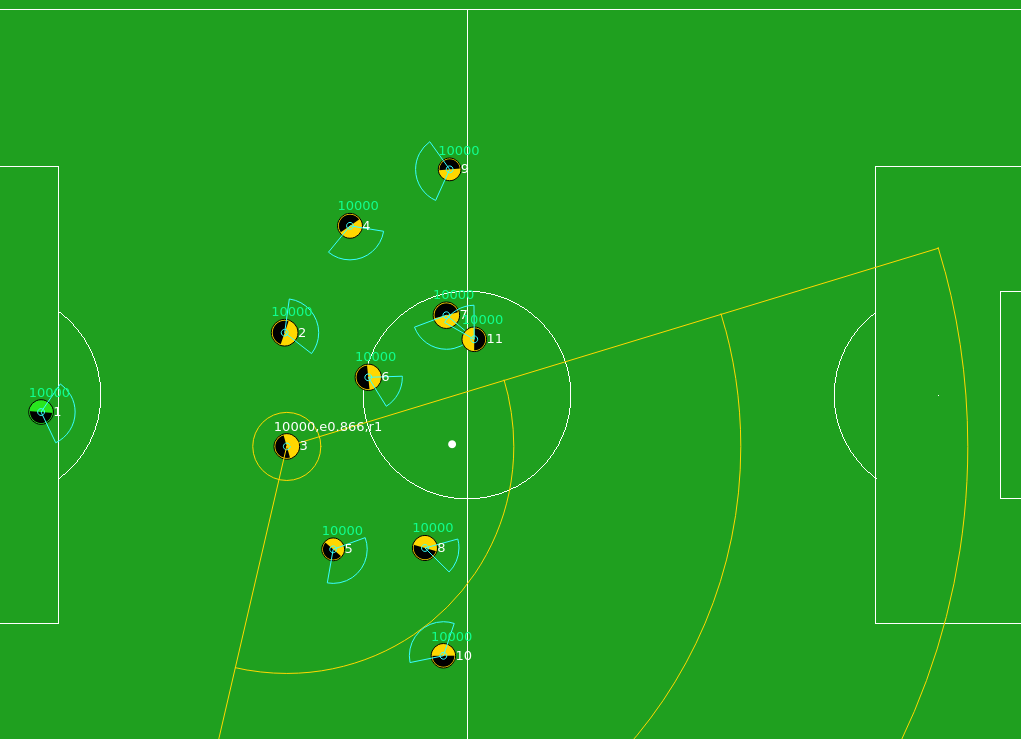
\includegraphics[width=0.75\textwidth]{images/view.png}
\caption{نمونه دید یک بازیکن. در این مثال، بازیکن ۳، بازیکن ۵ و ۸ و ۱۰ و توپ را می‌بیند و از موقعیت سایر بازیکنان اطلاعی ندارد.}\label{fig:view}
    
\end{figure}

هر عامل یک رزرو انرژی و یک منبع انرژی دارد. در صورت پر نبودن انرژی بازیکن، انرژی به نرخ ثابتی از رزرو به منبع منتقل می‌شود.
در صورت اتمام انرژی منبع، رفتار‌های بازیکن از جمله حرکت‌کردن کند‌تر می‌شوند.
رفتار‌های بیشتری (مانند تکل زدن، خطا و ضربه‌ آزاد، کارت زرد و قرمز و ...) 
نیز در محیط به کمک مدل‌های ریاضیاتی پیاده‌سازی شده‌است که خارج از دامنه این پروژه می‌باشد.

\section{کد پایه ایجنت}
در سال‌های اول مسابقات، هر تیمی کد عامل خود را از صفر می‌نوشت، که میزان در دسترس بودن لیگ را بسیار پایین آورده‌بود. با توجه به یکسان بودن بخش عمده‌ای از نیازمندی‌های تیم‌ها،
همچون نیاز به اتصال به سرور، نیاز به تفکیک وظایف بازیکنان به دروازه‌بان و مدافع و مهاجم، نیاز به موقعیت‌یابی اشیا در زمین، توابع هندسی، و ...، هیدهیسا آکیام از تیم هلیوس در سال ۲۰۱۲ تصمیم به ساختن یک کد پایه به صورت متن‌باز محض استفاده سایر تیم‌ها گرفت.
این کد پایه، که کد پایه ایجنت نام دارد، زیربنای ۱۳ تیم از ۱۵ شرکت‌کننده سال اخیر ربوکاپ بوده، و نقطه شروع اکثر کسانی است که قصد فعالیت در این فضا را دارند.
این کد پایه همچنان در حال به‌روز‌رسانی و تقویت‌شدن است
\LTRfootnote{\url{https://github.com/helios-base/helios-base}}
، و خود منشا سایر کد پایه‌های به اشتراک گذاشته‌شده همچون کد پایه گلایدرز\LTRfootnote{Gliders}
 و کد پایه سایرس\LTRfootnote{Cyrus}
  است.

با استفاده از این کد پایه، توسعه‌دهندگان می‌توانند سطح کدزدن خود را از سطوح پایین، به سطح استراتژی و تاکتیک و تصمیم‌گیری منتقل کنند. به طور مثال
بدون استفاده از یک کد پایه، برای حرکت عامل به مرکز زمین باید کد اتصال به سرور و موقعیت‌یابی را پیاده‌سازی کنیم. سپس درگیر مسائلی همچون محاسبه شتاب بازیکن، نیرویی که باید اعمال شود، مسیر حرکت بهینه (چرخیدن و دویدن یا دویدن مورب)
 و ... شوند. در حالی که این عمل، به صورت یک دستور سطح بالا در کد پایه ایجنت قابل اجراست. در بخش بعدی به تمام رفتار‌های ممکن در این کد پایه و سطح‌بندی رفتار‌ها می‌پردازیم.

\section{معرفی رفتار‌های ممکن}
هر عامل در هر لحظه، باید تصمیم‌گیری خود را به سرور بفرستد.
این تصمیم‌گیری می‌تواند شامل انجام یکی از رفتار‌های ممکن باشد.
در هر لحظه، عامل می‌تواند گردن خود را بچرخاند تا اطراف خود را ببیند، و همزمان یکی از پنج رفتار ضربه به توپ، حرکت بدن، چرخش بدن، تکل، یا گرفتن توپ را انجام دهد.
رایج است که رفتار‌های ممکن و پیاده‌سازی شده را به سه طبقه تقسیم‌بندی کنیم که در پایین‌ترین سطح، رفتار‌های سطح‌ سرور، و در بالا‌ترین سطح، رفتار‌های سطح استراتژیک و فکری
قرار می‌گیرند.
\subsection{رفتار‌های سطح پایین}
در پایین‌ترین سطح، رفتار‌ها مستقیما معادل با رفتار‌های مورد پذیرش سرور می‌باشند.
این رفتار‌ها شامل اعمال نیرو روی توپ در یک راستا (نسبت به بدن بازیکن)
 و نیروی خاص، 
 چرخاندن بازیکن به یک راستا،
اعمال نیروی حرکت بازیکن در راستا و نیرو،
تکل زدن در یک راستا،
و گرفتن توپ (در صورتی که بازیکن دروازه‌بان باشد)
می‌باشند.

\subsection{رفتار‌های سطح متوسط}
در این سطح، رفتار‌ها ساده‌سازی شده‌اند تا استفاده‌ از آن‌ها برای تصمیم‌گیری راحت‌تر باشد. 
به طور مثال رفتار حرکت به سمت یک نقطه‌ خاص از زمین،
رفتار ضربه زدن به توپ با سرعت دلخواه در راستای غیرنسبی،
رفتار ضربه زدن توپ به صورت چند‌ضرب به یک نقطه خاص،
و...
را می‌توان از رفتار‌های این سطح معرفی کرد.
\subsection{رفتار‌های سطح بالا}
در این سطح، رفتار‌ها حالت استراتژی و فکر کردن دارند، و به صورت انتزاعی و مشابه با فوتبال واقعی می‌باشند.
به طور مثال، حرکت به سمت نقطه‌ی آرایش\LTRfootnote{Formation}،
حرکت برای قطع توپ،
زدن شوت (در صورت ممکن بودن شوت موفق)،
و...
از رفتار‌های سطح بالا می‌باشند.
\section{حالت دید کامل}
همانطور که گفته‌شد، محیط اطلاعات کامل را در اختیار عامل قرار نمی‌دهد. با توجه به اینکه قصد تغییر کد سرور مسابقات و افزودن پاداش به سرور را نداریم، این محاسبات درون خود عامل باید صورت بگیرند.
خوش‌بختانه سرور مسابقات قابلیت ارسال محیط در حالت دید کامل
\LTRfootnote{Fullstate WorldModel}
 را دارد که در این حالت، همه اطلاعات بدون نویز به عامل ارسال می‌شوند.
 داخل کد ایجنت می‌توان انتخاب کرد که در صورت دریافت حالت دید کامل آن‌را جایگزین دید ناقص کند، یا اینکه هر دو را کنار هم نگه‌دارد.
 ما در فرآیند یادگیری تقویتی از حالت دوم استفاده می‌کنیم تا با کمک دید کامل محاسبات پاداش را انجام دهیم، و با حالت دید ناقص تصمیم‌گیری کنیم.
در عکس \ref{fig:ss2d_rl_loop} می‌توان مشاهده کرد که پاداش داخل عامل محاسبه‌شده، و تابعی از حالت دید کامل (\lr{Fullstate} یا به اختصار \lr{FS})
است، و محیط هر دو حالت دید را برای عامل ارسال می‌کند.
این نمودار در واقع حالت اصلاح‌شده \ref{fig:agent_env} است که خاص‌منظوره این پروژه می‌باشد.
 \begin{figure}[H]
    \centering
    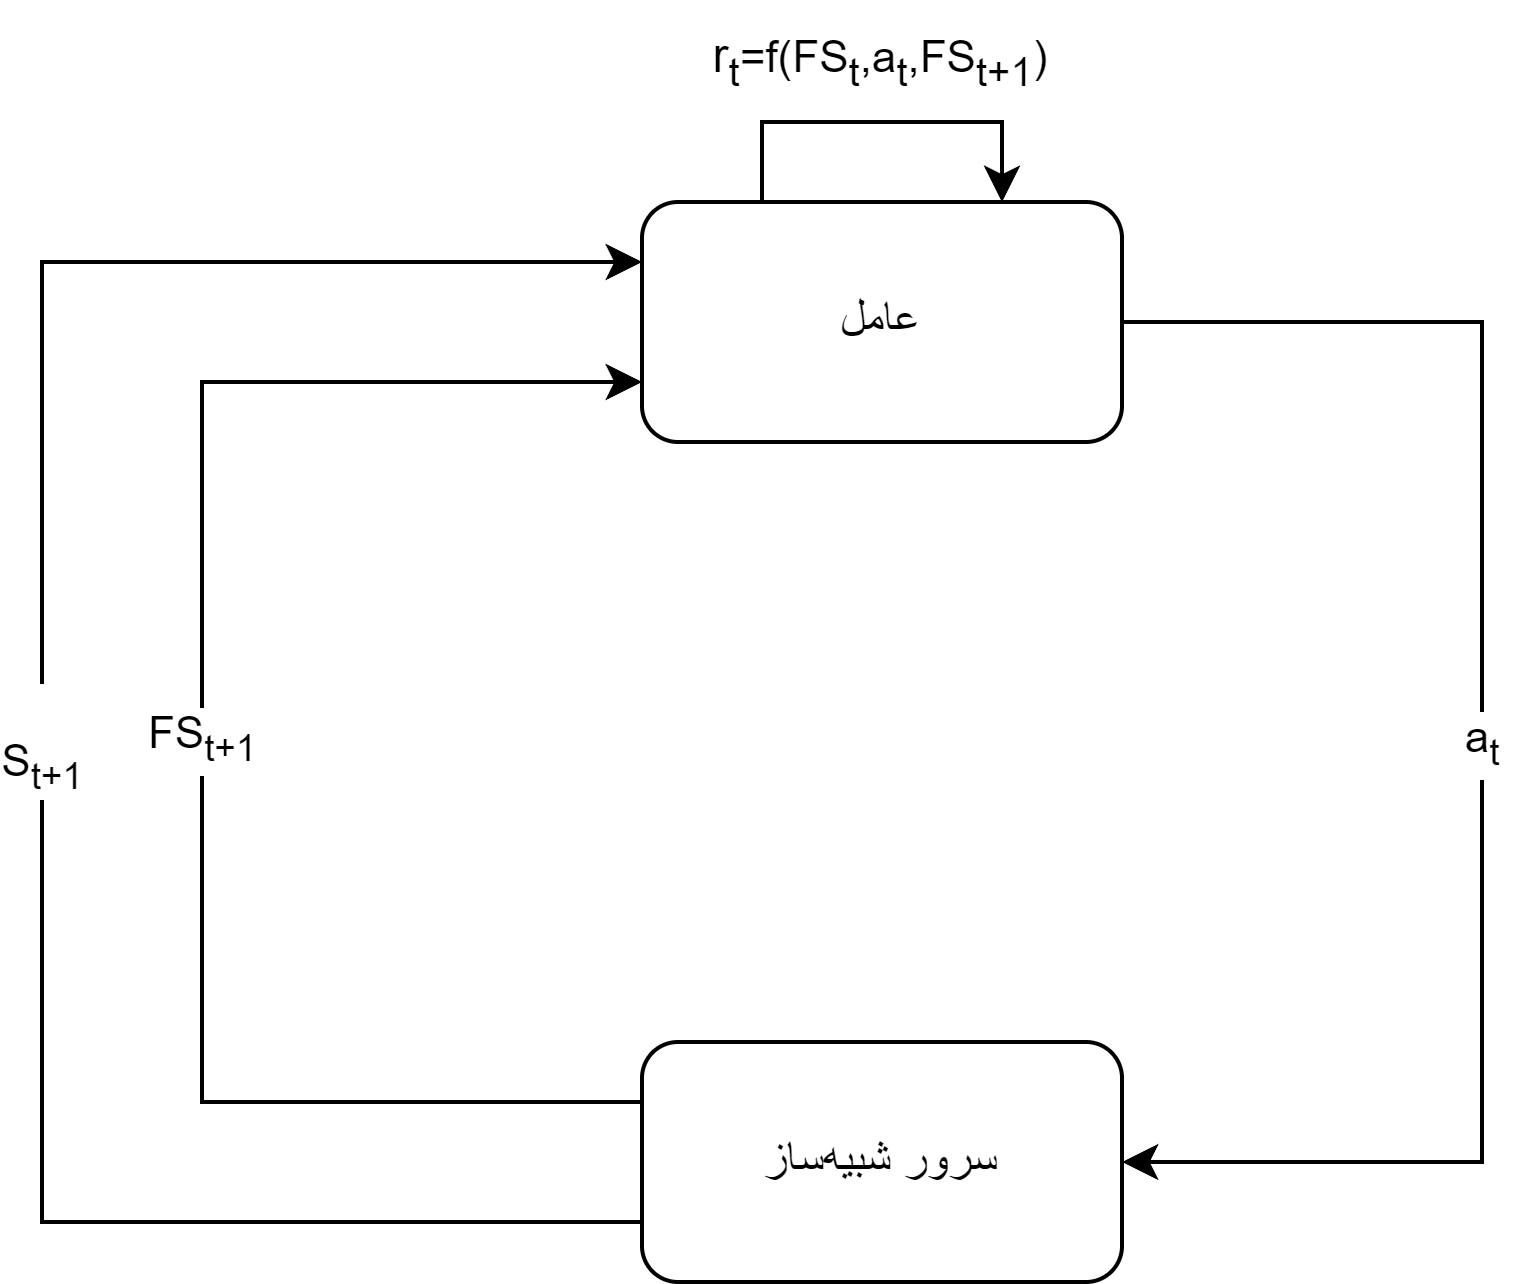
\includegraphics[width=0.75\textwidth]{images/ss2d_reward.png}
    \caption{ارتباط بین محیط و عامل، و روش محاسبه پاداش}\label{fig:ss2d_rl_loop}
 \end{figure}
\section{معرفی حالت پنالتی}
در صورت تساوی بازی در ده دقیقه زمان عادی، و تداوم تساوی پس از وقت اضافی، بازی به حالت پنالتی می‌رود. 
با توجه به دو بعدی بودن محیط، در صورتی که مشابه با فوتبال واقعی، پنالتی به صورت تک ضرب باشد، می‌توان برای آن استراتژی قطعی ارائه داد.
به همین منظور، پنالتی در فضای لیگ دو‌بعدی، به صورت تک به تک با دروازه‌بان است.

بازیکن مهاجم، ۱۵ ثانیه فرصت دارد تا توپ را به گل تبدیل کند. دروازه‌بان باید در این مدت تلاش کند جوری موقعیت‌گیری کند که حریف نتواند شوت منجر به گل داشته‌باشد.
در صورتی که زمان مهاجم تمام شود، توپ به بیرون محیط بازی برود، یا توپ توسط دروازه‌بان گرفته‌شود، دروازه‌بان برنده می‌شود. در صورتی که توپ وارد گل شود، مهاجم برنده می‌شود.

با توجه به تک‌عامله بودن، و محدود بودن زمان محیط، می‌توان از روش‌های یادگیری تقویتی برای یادگیری استراتژی‌های بهینه برای پنالتی استفاده کرد.
در شکل
\ref{fig:penalty_demo}
 یک نمونه از حالت پنالتی را مشاهده می‌کنید.
\begin{figure}[H]
\centering
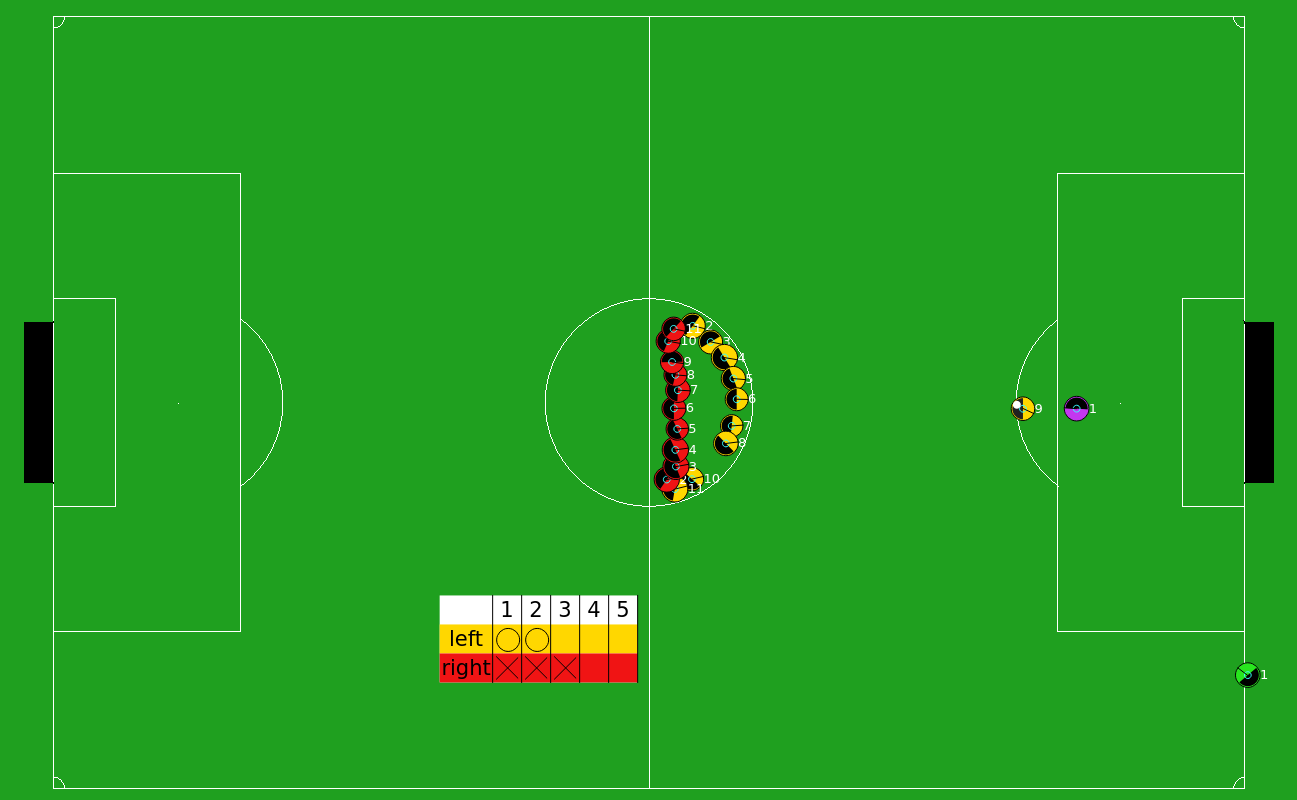
\includegraphics[width=0.75\textwidth]{images/penalty.png}
\caption{نمونه‌ای از بازی در حالت پنالتی}\label{fig:penalty_demo}
\end{figure}
\section{کار با مربی تمرینی برای تولید محیط‌ قابل تکرار}
با توجه به اینکه برای یادگیری تقویتی، نیاز به بازگرداندن محیط به حالت اولیه را داریم، می‌توانیم از 
مربی تمرینی\LTRfootnote{Trainer}
استفاده کنیم.
در صورتی که در تنظیمات سرور، این حالت فعال شده باشد، می‌توان کدی نوشت که در شرایط دلخواه، توپ و بازیکنان را جا‌به‌جا کنیم،
حالت بازی را تنظیم کنیم، انرژی بازیکنان را پر کنیم‌ و ... .
در فصل‌های آینده از این امکان، برای ساختن یک رابط استاندارد یادگیری تقویتی برای محیط فوتبال استفاده خواهیم کرد.
\section{جمع‌بندی}
در این فصل، محیط فوتبال ربوکاپ دوبعدی به عنوان یک ابزار مطالعاتی برای تقویت پیشرفت‌ها در زمینه هوش مصنوعی و رباتیک معرفی شد.
این محیط، با ارائه یک پلتفرم مسابقه‌ای مبتنی بر قوانین فوتبال واقعی، فرصت‌هایی برای توسعه و آزمایش الگوریتم‌های تصمیم‌گیری، هماهنگی، و استراتژی در محیط‌های چندعامله فراهم می‌کند.

معرفی این محیط شامل توضیح قوانین بازی، نحوه ارتباط و تصمیم‌گیری عامل‌ها، و همچنین ساختار کد پایه ایجنت بود که توسعه‌دهندگان را قادر می‌سازد تا تمرکز خود را بر روی تاکتیک و تصمیم‌گیری‌های سطح بالای مشابه با فوتبال معطوف دارند.

یکی از نوآوری‌های کلیدی در این فصل، استفاده از حالت دید کامل در کنار دید ناقص است که به عامل‌ها امکان می‌دهد تا پاداش‌ها را بر اساس اطلاعات کامل محیط محاسبه کنند، در حالی که تصمیم‌گیری بر اساس دید ناقص انجام می‌شود. این رویکرد یک قدم مهم در راستای افزایش قابلیت‌های یادگیری تقویتی در محیط‌هایی با دید ناقص است.

همچنین، با معرفی حالت پنالتی و استفاده از مربی تمرینی برای تولید محیط‌های قابل تکرار، زمینه‌های لازم برای پیاده‌سازی الگوریتم‌های یادگیری تقویتی فراهم شده است. این امکانات به پژوهشگران اجازه می‌دهد تا در یک محیط مسابقه‌ای استاندارد، استراتژی‌های بهینه‌سازی شده را آزمایش و توسعه دهند.
\chapter{پیاده‌سازی و آماده‌سازی محیط استاندارد}
\section{زیرساخت پایتونی تهاجم نصف زمین}
در سال ۲۰۱۵، 
پروژه تهاجم نصف زمین \LTRfootnote{Half Field Offense (HFO)} یا همان اچ‌اف‌او
تلاش کرد محیط پایتونیی برای یادگیری تقویتی در فوتبال دو بعدی ایجاد کند.
کد سرور به گونه‌ای تغییر یافته‌بود، که بازیکن بتواند به سرور دستور اعمال رفتار‌ها و رفتن به گام بعدی را بدهد.

این روش متکی بر قابلیت‌های لیب‌سی \LTRfootnote{LibC} بود، که از آن برای ارتباط با کد \lr{cpp} استفاده می‌کرد.
لیب‌سی اجازه می‌دهد که اگر کلاس معادل پایتونی و \lr{cpp} وجود داشته باشد،
از سمت پایتون می‌توان به آن دسترسی داشت.
در این پروژه، عامل پایتونی به عنوان ایجنت دسترسی به محیط دارد، که با آن از کد \lr{cpp} محیط را درخواست می‌کند.
محیط در دو سطح بالا و پایین قابل درخواست است؛ حالت سطح پایین ۶۰ ویژگی محیط، و حالت سطح بالا ۹ ویژگی را به صورت یک آرایه صفر تا یک به عامل پس می‌دهد.
عامل سپس تصمیم خود را اخذ کرده، و به سرور دستور اجرای آن را می‌دهد.
معایب استفاده از این محیط عبارت بود از:
\begin{itemize}
    \item دشواری در تغییر محیط عامل به صورت دلخواه
    \item تفاوت زیاد بین محیط آماده‌شده در ایجنت، که مورد استفاده اکثر تیم‌هاست، و محیط اچ‌اف‌او
    \item عقب‌ماندگی محیط به علت تغییر کد‌های سرور و به روز نبودن با تغییرات شبیه‌ساز
    \item دشواری نصب، به علت پیش‌نیاز‌های قدیمی همچون \lr{Qt4}
    \item عدم امکان استفاده از تیم‌های جدید برای حریف یادگیری به علت نسخه قدیمی سرور
\end{itemize}
\section{کد پایه پایرس}
با توجه به دشواری استفاده از یادگیری ماشین در \lr{CPP}،
ما در تیم سایرس تصمیم به پیاده‌سازی یک کد پایه معادل با کد پایه \lr{Agent2D}
در پایتون گرفتیم، که نام آن پایرس \LTRfootnote{Pyrus} است.\cite{Pyrus2D}
این تلاش‌ها از سال ۲۰۱۹ آغاز شد و در نهایت بعد از سه سال و حدود ۲۵ هزار خط کد، پروژه به حالت پایدار و قابل استفاده رسیده‌است.\LTRfootnote{\url{https://github.com/Cyrus2D/Pyrus2D}}

امید بر آن بود که با توجه به اتکا بر الگوریتم‌های یادگیری ماشین به‌جای الگوریتم‌های درخت و گراف، بتوان کندی زبان پایتون را جایگزین کرد.
در کد \lr{Agent2D}،
قبل از رسیدن به گام تصمیم‌گیری، محاسبات زیادی رخ می‌دهد تا بازیکن موقعیت خود و سایر بازیکنان را بیابد، سریعترین بازیکنان به توپ، موقعیت آفساید و... را به دست آورد.
با توجه به کند بودن پایتون در مقایسه با \lr{cpp}،
همین محاسبات مقدماتی نیز بسیار زمان‌بر بودند و بخش بزرگی از ۱۰۰ میلی‌ثانیه موجود برای هر گام بازی را اشغال می‌کردند.
به همین منظور، پایرس جایگزین مناسبی برای پایتونی کردن کد نبود.

\begin{figure}[H]
    \centering
    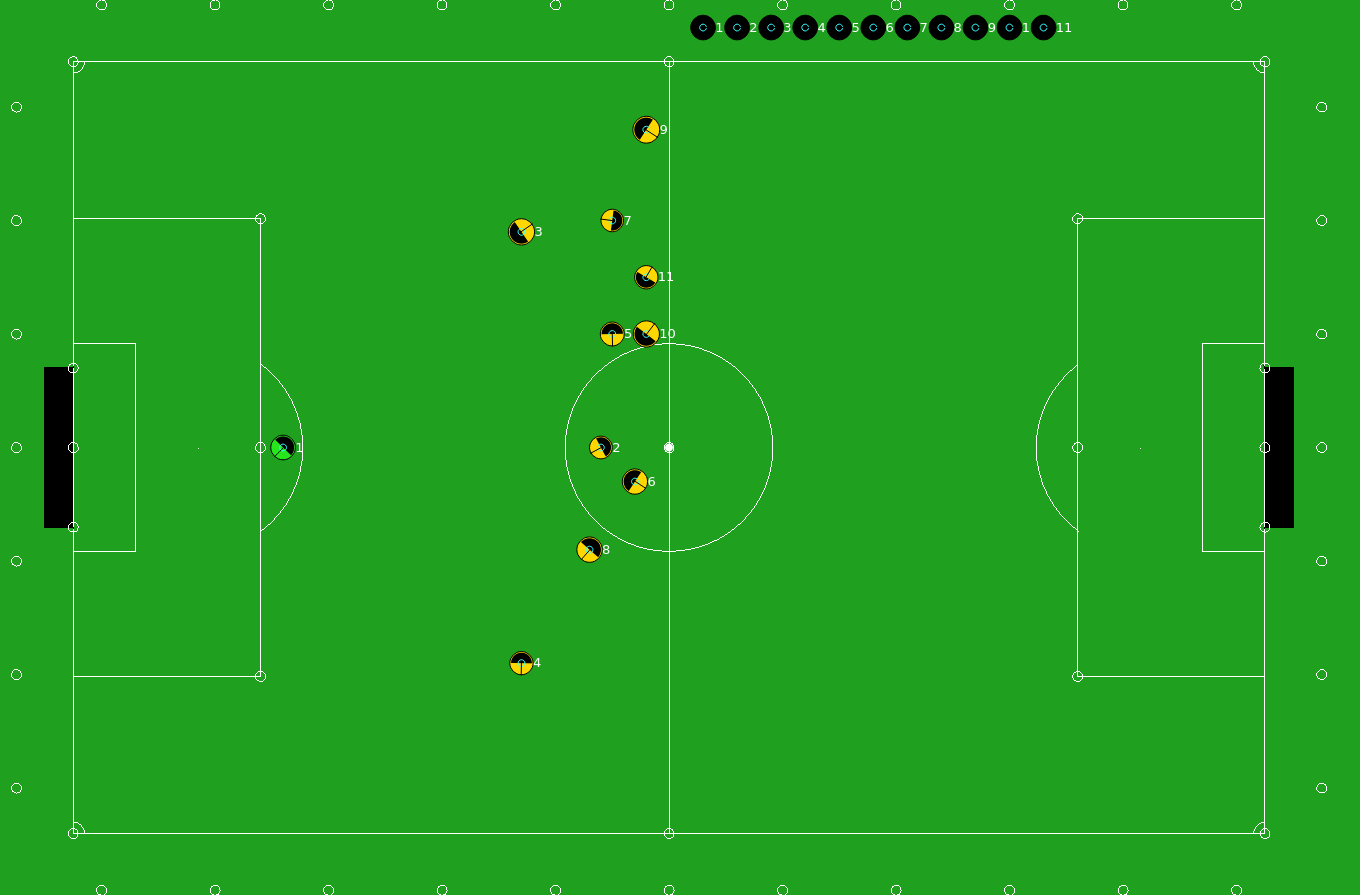
\includegraphics[width=0.75\textwidth]{images/flags.png}
    \caption{پرچم‌های کنار زمین، که برای موقعیت‌یابی استفاده می‌شوند.}\label{fig:flags}
    
\end{figure}

\section{کد پایه جی‌آر‌پی‌سی}
% TODO add grpc explanation
با توجه به سریع بودن \lr{cpp} 
برای پیش‌پردازش،
و کاربردی و راحت بودن پایتون برای یادگیری تقویتی،
تصمیم گرفتیم به کمک پروتکل فراخوانی تابع از راه دور \LTRfootnote{Remote Procedure Call (RPC)}،
این دو زبان را به هم متصل کنیم.
 در این پروژه از چارچوب فراخوانی تابع از راه دور گوگل، یا همان جی‌آر‌پی‌سی \LTRfootnote{gRPC (google Remote Procedure Call)}
 استنفاده می‌کنیم.

در این چارچوپ، ابتدا یک فایل پروتو \LTRfootnote{Proto} 
باید تعریف کرد، که حاوی مشخصات اشیاء و امضای توابع است. سپس با استفاده از کامپایلر پروتو می‌توان کد‌های سرور و کلاینت را به زبان‌های دلخواه تبدیل کرد.
سپس با اضافه کردن کد تولید‌شده توسط کامپایلر پروتو می‌توان درون کلاینت از توابع به‌گونه‌ای استفاده کرد که گویا داخل خود کد قرار دارند. از مهم‌ترین مزایای
این پروتکل ارتباطی، مستقل از زبان بودن آن، و نوشتن بسته‌های پیام به صورت صفر و یکی (در مقابل متنی)  است که سربار زمانی نوشتن و خواندن پیام را ناچیز می‌کند.
همچنین به علت استفاده از پروتکل اچ‌تی‌تی‌پی \LTRfootnote{HTTP} برای ارسال بسته‌ها روی شبکه، 
می‌توان از ضمانت‌های دریافت پیام نیز استفاده کرد.
\begin{figure}[H]
    \centering
    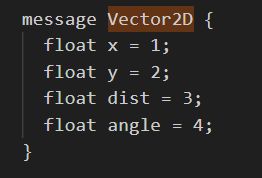
\includegraphics[width=0.4\textwidth]{images/grpc_message.png}
    \caption{نحوه تعریف اشیا در جی‌آر‌پی‌سی}\label{fig:grpc_message}
\end{figure}
\begin{figure}[H]
    \centering
    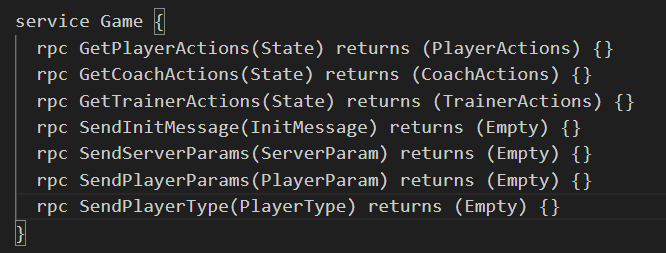
\includegraphics[width=0.75\textwidth]{images/grpc_service.png}
    \caption{نحوه تعریف توابع در جی‌آر‌پی‌سی}\label{fig:grpc_service}
\end{figure}

برای تشکیل اتصال بین این دو زبان کد پایه \lr{Agent2D} را به‌گونه‌ای تغییر دادیم که
پس از اتمام مراحل پیش‌پردازش و آماده شدن مدل دنیای بازیکن\LTRfootnote{WorldModel}
در \lr{cpp}،
اطلاعات آن را با یک درخواست جی‌آرپی‌سی
به یک سرور تصمیم‌گیری پایتونی بفرستد.
در شکل \ref{fig:connection} و \ref{fig:grpc_base}
نحوه‌ی اتصال اجزای مسابقه، و روند عمومی تصمیم‌گیری نمایش داده شده‌است.

\begin{figure}[H]
    \centering
    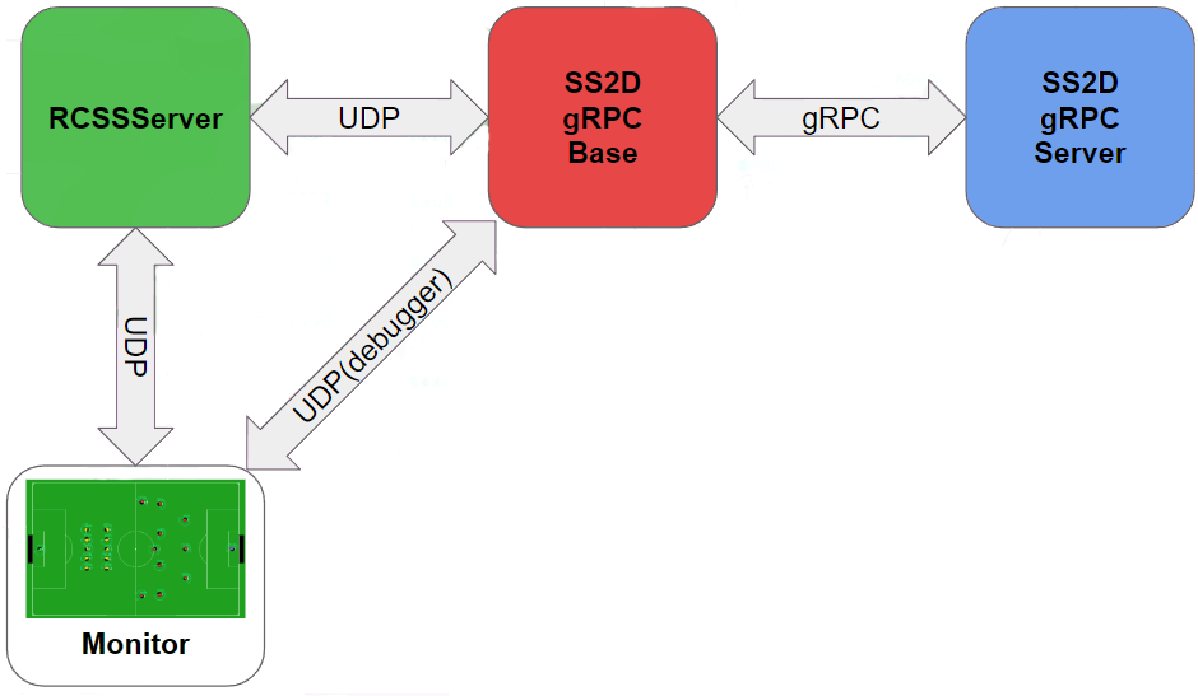
\includegraphics[width=0.75\textwidth]{images/connection_protocols.png}
    \caption{پروتکل‌های استفاده‌شده برای ارتباط بین اجزای مسابقه}\label{fig:connection}
    
\end{figure}

\begin{figure}[H]
    \centering
    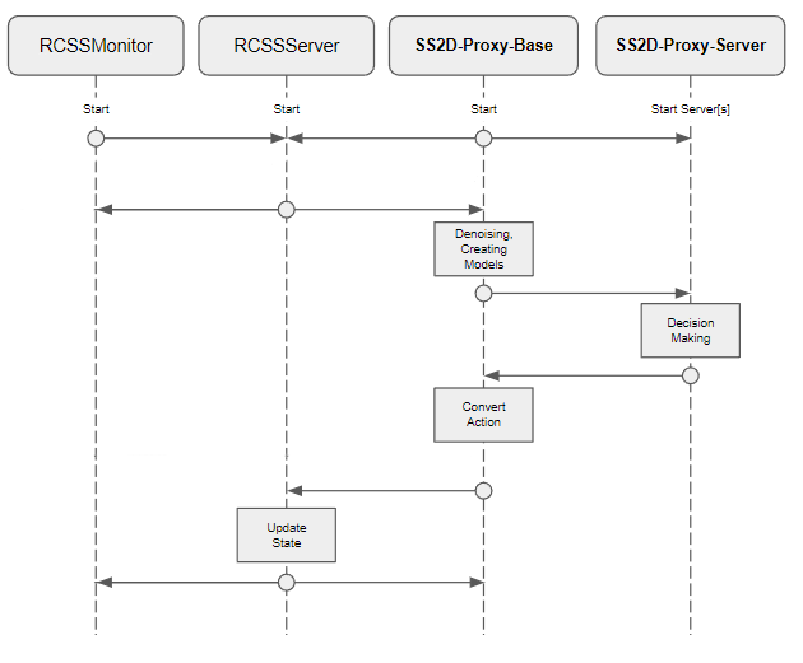
\includegraphics[width=1\textwidth]{images/grpc_base.png}
    \caption{نحوه کارکرد و اتصال کد پایه جی‌آر‌پی‌سی به سرور مسابقات و نمایشگر بازی}\label{fig:grpc_base}
    
\end{figure}
\section{محیط استاندارد جیم}
پلتفرم جیم \LTRfootnote{Gym}
که توسط گروه اپن‌ای‌ای \LTRfootnote{OpenAI}
توسعه داده شده‌است،
یک محیط استاندارد برای یادگیری تقویتی است.
این پلتفرم شامل محیط‌های گوناگون از پیش آماده شده است که می‌توانند برای یادگیری تقویتی استفاده شود.
این محیط همچنین به ما قابلیت تعریف محیط‌های جدید را می‌دهد.
\begin{figure}
    \centering
    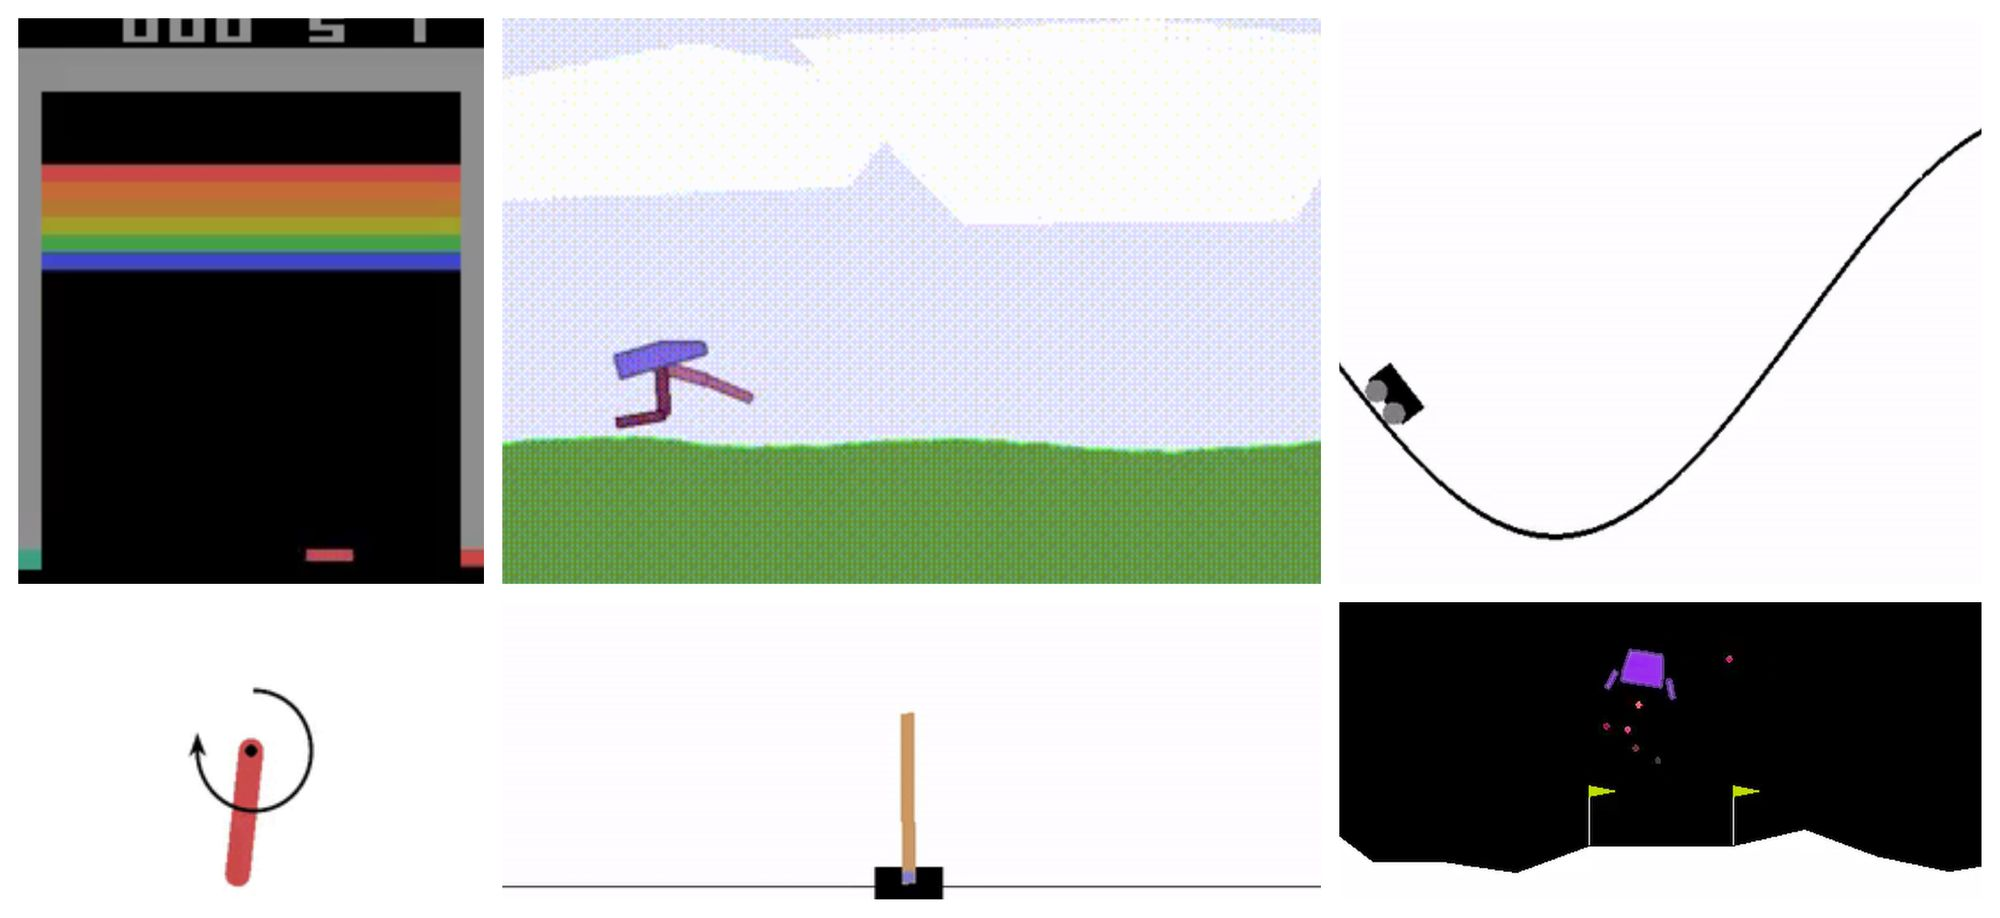
\includegraphics[width=0.75\textwidth]{images/openaigym.jpg}
    \caption{نمونه‌ای از محیط‌های آماده شده در پلتفرم جیم}\label{fig:gym}
    
\end{figure}
در سال ۲۰۲۳، 
مدیریت و نگه‌داری این پلتفرم به شرکت فاراما \LTRfootnote{Farama}
واگذار شد و از آن زمان، این پلتفرم به نام پلتفرم جیمنازیوم \LTRfootnote{Gymnasium}
 شناخته می‌شود.
تبدیل محیط یادگیری به این نوع محیط، نه تنها به ما قابلیت استفاده از کتاب‌خانه‌های پیشین و کمک گرفتن از ابزار‌های
از پیش تعبیه شده را می‌دهد، بلکه امکان به اشتراک‌گذاری راحت این محیط به سایر محققان را نیز فراهم می‌کند.
\subsection{توصیف رابط و توابع موجود}
برای تعریف یک محیط جدید در جیم،
باید توابع استاندارد آن را پیاده‌سازی کنیم. به این منظور، لازم است با روش کارکرد هر جزء محیط آشنا شویم.
لازم به ذکر است که تفاوت‌های جزئیی بین نسخه اوپن‌ای‌ای و فاراما وجود دارد، که در اینجا به توصیف نسخه فاراما می‌پردازیم.
\subsubsection{تابع گام برداشتن}
این تابع، یک عمل را به عنوان ورودی می‌گیرد،
و وضعیت جدید، پاداش این عمل، و اطلاعاتی همچون اتمام بازی، یا تمام شدن وقت عامل را به عنوان خروجی برمی‌گرداند.
\subsubsection{تابع شروع مجدد}
این تابع، محیط را به حالت اولیه باز می‌گرداند، و حالت جدید را به عامل برمی‌گرداند.
در صورتی که شروع بازی شامل المان‌های تصادفی باشد، ورودی این تابع باید کاوش تصادفی \LTRfootnote{Random Seed} را نیز به عنوان ورودی بگیرد.
\subsubsection{انواع فضا‌های حالت و عمل}
در حین تعریف محیط، باید فضا‌های حالت و عمل را نیز تعریف کنیم.
هر فضا می‌تواند از انواع زیر باشد:
\begin{itemize}
    \item گسسته \LTRfootnote{Discrete}: به ازای ورودی \lr{n}، در این فضا می‌توانیم از اعداد صحیح از ۰ تا \lr{n-1} استفاده کنیم.
    این حالت بیشتر برای فضای خروجی استفاده می‌شود.
    \item گسسته چند‌تایی \LTRfootnote{MultiDiscrete}: این فضا مشابه فضای گسسته است، با این تفاوت که می‌توانیم چند عدد از این فضا را به عنوان خروجی بگیریم.
    مشابه با گسسته است، ولی جای ورودی یک عدد، یک آرایه از اعداد است؛ هر عدد نشان‌دهنده تعداد حالت‌های ممکن در هر بعد است.
    \item فضای بسته \LTRfootnote{Box}: نشان‌دهنده یک فضای چند‌بعدی پیوسته است، که باید حد پایین و بالای هر بعد را مشخص کنیم.
    \item دوتایی چند‌بعدی \LTRfootnote{MultiBinary}: حالت چند‌بعدی است، که هر بعد مقدار صفر یا یک می‌تواند به‌خود بگیرد.
\end{itemize}
به کمک فضا‌های فوق، می‌توان فضا‌هایی از ترکیب حالت‌های فوق تعریف کرد، که به انواع زیر است:
\begin{itemize}
    \item دیکشنری \LTRfootnote{Dict}: یک دیکشنری پایتونی از فضا‌های مختلف است.
    \item چندتایی (توپل) \LTRfootnote{Tuple}: یک چندتایی مرتب از فضا‌های مختلف است.
    \item دنباله \LTRfootnote{Sequence}: یک دنباله از فضا‌های مختلف است.
\end{itemize}

\subsubsection{تابع پایان}
در اتمام کار با محیط، این تابع فراخوانی می‌شود تا محیط بسته شود، و منابع آن آزاد شوند.
\subsubsection{تابع ترسیم}
با توجه به اینکه اکثر محیط‌های جیم، به کمک کتاب‌خانه‌هایی مانند \lr{PyGame}
ترسیم می‌شوند، این تابع برای ترسیم محیط در هر گام استفاده می‌شود.
همچنین به عنوان ورودی این تابع می‌توان معین کرد که ترسیم به چه گونه‌ای انجام شود، چرا که ممکن است در حین آموزش برای تسریع عملیات، نیازی به ترسیم نباشد.
از آن‌جا که در محیط ما، وظیفه ترسیم با نمایش‌گر خارجی انجام می‌شود، این تابع برای ما معنی ندارد. 
\subsection{نحوه ادقام با فضای ربوکاپ}
برای پیاده‌سازی محیط جیم در فضای ربوکاپ، از کد پایه \lr{gRPC} استفاده می‌کنیم.
فرآیند سرو کردن درخواست‌های این پروتکل را با کمک کتاب‌خانه‌های استاندارد پایتون به یک رشته \LTRfootnote{Thread}
جدا منتقل می‌کنیم، که با کمک دو صف با رشته محیط جیم ارتباط دارد.
در هنگام دریافت حالت از بخش پایه \lr{cpp}،
رشته سرویس‌دهنده حالت را داخل صف مشاهدات می‌گذارد، و منتظر می‌شود که رشته جیم، تصمیم عامل را بر اساس مشاهده ثبت‌شده در صف عمل‌ها قرار دهد.
صف سومی نیز برای سرمربی وجود دارد، که در صورت نیاز به شروع مجدد محیط، از سمت جیم پر می‌شود. 
کد سرمربی تمرینی در هر لحظه از اجرایش چک می‌کند و در صورت خالی نبودن صف، دستورات لازم برای از نو کردن محیط را می‌فرستد. در صورت خالی بودن صف نیز عمل خالی به کد پایه پس می‌فرستد.

\begin{figure}[H]
    \centering
    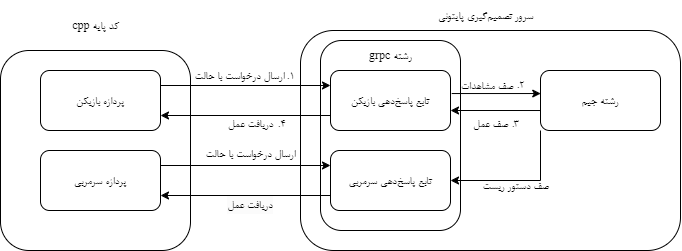
\includegraphics[width=1\textwidth]{images/grpc_gym.png}
    \caption{نحوه کلی ارتباط کد پایه، تصمیم‌گیرنده جی‌آر‌پی‌سی و جیم}\label{fig:gym_grpc}
\end{figure}
در شکل \ref{fig:gym_timing}
به طور دقیق می‌توان ترتیب فراخوانی توابع، و نحوه استفاده از محیط جیم را مشاهده کرد.
کد اجرا کننده \LTRfootnote{Driver Code}
دقیقا فرم مشابه سایر محیط‌های جیم را دارد و از این رابط به طور کامل طبعیت می‌کند.
بخش‌های قرمز رنگ به معنی قفل بودن رشته‌ی اجرایی و در انتظار ماندن برای محتویات صف است.
\begin{figure}[H]
    \centering
    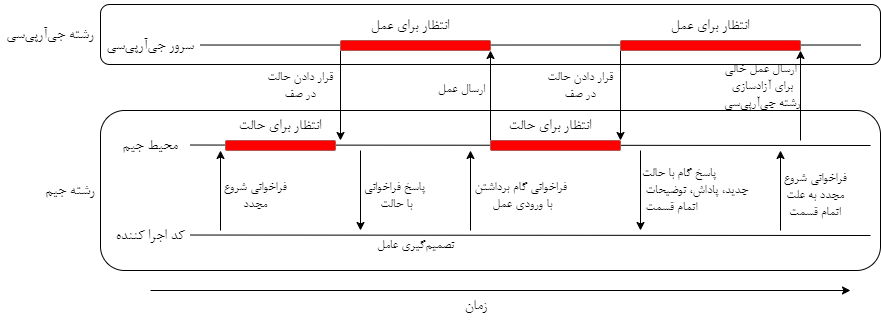
\includegraphics[width=1\textwidth]{images/timing.drawio.png}
    \caption{ترتیب فراخوانی توابع برای اجرای جیم با سرور ربوکاپ}\label{fig:gym_timing}
\end{figure}

داخل شکل، یک قسمت که فقط یک گام تصمیم‌گیری دارد را می‌توان دید. در واقعیت مراحل ((گام برداشتن))
تا قبل از ((فراخوانی شروع مجدد))
به تعداد گام‌های قسمت، تکرار می‌شوند.

برای محیط پنالتی، در صورتی که توپ قابل ضربه‌زدن نباشد، حرکت صحیح همیشه قطع توپ با حداکثر سرعت برای ضربه مجدد است. بنابرین فقط حالت را در شرایطی به جیم ارسال می‌کنیم که توپ قابل ضربه‌زدن باشد.
\subsection{فضای حالت و فضای عمل عامل}
\subsubsection{فضای حالت}
فضای حالت انتخاب‌شده یک بسته ۹ بعدی است، که شامل ویژگی‌های زیر می‌باشد: موقعیت قطبی بازیکن نسبت به مرکز دروازه (اندازه و زاویه)،
موقعیت دکارتی توپ‌ (ایکس و ایگرگ)،
موقعیت دکارتی دروازه‌بان (ایکس و ایگرگ)،
زاویه نسبی حریف نسبت به توپ،
موقعیت قطبی دروازه‌بان نسبت به بازیکن (اندازه و زاویه).

علت اهمیت عاملی مثل زاویه بدن دروازه‌بان، قابلیت حرکت سریع‌تر بازیکنان در راستای مستقیم است. می‌توان عواملی هم‌چون سرعت بازیکنان را نیز اثر داد،
اما برای همگرایی بهتر و سریع‌تر از این عوامل صرف نظر شده.
\subsubsection{فضای عمل}
همان‌طور که گفته‌شد، عامل به صورت خودکار به دنبال توپ می‌رود و ما با کمک یادگیری تقویتی قرار است این عامل را به یادگیری ضربه‌زدن به دروازه برسانیم.
برای این منظور، از رفتار سطح متوسط ضربه با سرعت دلخواه در راستای دلخواه (\lr{KickOneStep})
 استفاده می‌کنیم تا محاسبات مستقل از سرعت توپ قبلی و شتاب توپ شوند.

 به این منظور، فضای عمل ما نیاز است سرعت و زاویه ضربه را تعیین کند.
 با توجه به اینکه برخی الگوریتم‌ها مانند \lr{DQN} بهترین عمل را از بین اعمال ممکن انتخاب می‌کنند و نیاز به فضای عمل گسسته دارند،
و سایر الگوریتم‌ها مانند \lr{DDPG} نیاز به فضای عمل پیوسته دارند،
محیط را در دو حالت گسسته و پیوسته پیاده‌سازی کردیم.

در فضای پیوسته، دو مقدار سرعت توپ و زاویه ضربه به عامل داده می‌شود.
سرعت توپ بین صفر تا یک می‌باشد که نشان‌دهنده سرعت توپ نسبت به حداکثر سرعت ممکن است.
زاویه ضربه بین منفی یک تا یک می‌باشد که نرمال‌شده زاویه مطلق ضربه بین \lr{-۱۸۰} تا ۱۸۰ درجه است.

در حالت گسسته نیز، خروجی ما سرعت توپ و زاویه‌است، اما به‌جای مقادیر پیوسته، زوایای ضربه ممکن را به ۱۲ قسمت مساوی تقسیم کرده‌ایم و سرعت توپ را به ۱۰ قسمت مساوی تقسیم کرده‌ایم.
می‌توان این تقسیم‌بندی را به راحتی تغییر داد و تاثیرات آن روی سرعت یادگیری و نتیجه نهایی آن را بررسی کرد.
در شکل \ref{fig:discretization} می‌توان یک نمونه از تقسیم‌بندی فضای عمل را مشاهده کرد.
از آنجا که سرعت به ۲ درجه تقسیم شده‌است، حالت‌های ممکن آن معادل با نصف حداکثر سرعت توپ و حداکثر سرعت توپ می‌باشد.
\begin{figure}[H]
    \centering
    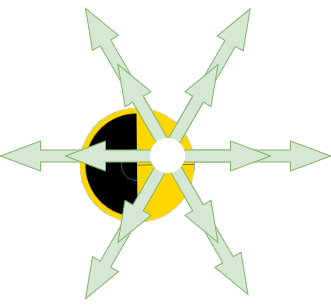
\includegraphics[width=0.45\textwidth]{images/discretization.drawio.png}
    \caption{تقسیم‌بندی فضای عمل به ۶ زاویه و ۲ سرعت}\label{fig:discretization}
\end{figure}
\subsection{طراحی پاداش}
همان‌طور که گفته شد، محیط جیم در حالت‌هایی که توپ قابل ضربه‌زدن است، یا توپ به بیرون رفته و یا توسط دروازه‌بان گرفته‌شده اجرا می‌شود.
در این حالت‌ها باید بر اساس شرایط قبلی، عمل و شرایط جدید پاداشی محاسبه کنیم که به عامل کمک می‌کند تا راحت‌تر به هدف خود نزدیک شود.
\subsubsection{پاداش‌های پایانی}
همانطور که گفته‌شد، چهار حالت پایانی داریم:
\begin{enumerate}
    \item حالت گل زدن: با توجه به رسیدن به هدف، پاداش بزرگی به عامل می‌دهیم که این مقدار، ۱۵۰۰ فرض شده‌است.
    \item حالت بیرون رفتن توپ: از آن‌جا که تنها با ضربات بد این سناریو رخ می‌دهد، پاداش بسیار بزرگ منفی \lr{-۵۰۰} دارد.
    \item گرفتن توپ توسط دروازه‌بان: این حالت از آنجا که بهتر از بیرون رفتن توپ است، پاداش منفی کوچک‌تری دارد و مقدار \lr{-۲۰۰} دارد.
    \item حالت اتمام زمان: به این حالت، پاداش \lr{-۱۵۰} تخصیص داده‌شده، تا عامل در حالتی که هنوز به گل‌زدن نرسیده‌است، مستقیما توپ را به دروازه‌بان ندهد. در واقع با کوچک‌تر در نظر گرفتن این پاداش، عامل را به کاوش بیشتر وا‌می‌داریم.
\end{enumerate}
\subsubsection{پاداش در حالت عادی}
در حالت بین دو ضربه، پاداش را بر اساس سه فاکتور حساب می‌کنیم:
\begin{itemize}
    \item می‌خواهیم عامل را به حرکت به سوی دروازه واداریم، پس از تفاضل فاصله توپ با دروازه در حالت جدید و حالت قبلی به عنوان معیار اصلی استفاده می‌کنیم. در واقع از عکس این فاکتور استفاده می‌کنیم، چرا که کاهش فاصله ویژگی مثبتی است.
    \item نزدیک شدن زیادی به دروازه‌بان ویژگی خوبی نیست، پس از ضریبی از تفاضل فاصله توپ با دروازه‌بان در بین دو حالت استفاده می‌کنیم.
    \item پاداش ثابت \lr{-۱۰} که برای تشویق عامل برای سریع‌تر رسیدن به حالت گل می‌باشد. از این رو که عامل این پاداش را فقط در لحظات ضربه زدن می‌بیند، این فاکتور عامل را به زدن ضربات با قدرت بیشتر تشویق می‌کند.
\end{itemize}
\section{پیاده‌سازی یادگیری تقویتی}
\subsection{پیاده‌سازی شبکه کیو عمیق}
با کمک کتاب‌خانه \lr{PyTorch}،
یک شبکه عصبی با یک لایه پنهان و تابع فعال‌سازی \lr{ReLU} پیاده‌سازی شد.
این شبکه، ورودی به ابعاد فضای حالت محیط دارد و خروجی به اندازه فضای عمل است.
تمامی ابرپارامتر‌های ما به عنوان ورودی تابع سازنده مدل داده می‌شوند.

سپس تابع یادگیری فراخوانی می‌شود، که ورودی آن مشخص می‌کند که چند گام از محیط برای آموزش استفاده شود.
این تابع، با استفاده از الگوریتم \lr{DQN}،
به تعداد مراتب در محیط گام بر می‌دارد و تجارب را به بافر اضافه می‌کند. در گام‌هایی که شماره آن ضریبی از ابرپارامتر \lr{update\_freq} است،
شبکه را به کمک گزینش ریزدسته‌ای از تجربیات و الگوریتم گرادیان، به‌روز می‌کند.
همچنین در گام‌هایی که شماره آن ضریبی از ابرپارامتر \lr{target\_update\_freq} است،
شبکه هدف را به‌روز می‌کند.

همانطور که در فصل‌های قبل اشاره شد، نرخ کاوش تصادفی به مرور زمان کاهش می‌یابد.
در ابرپارامتر‌ها، نرخ اولیه، نرخ نهایی، و درصد گام‌هایی که این کاهش نرخ در آن رخ می‌دهد با 
پارامتر‌های \lr{epsilon\_start}، \lr{epsilon\_end} و \lr{epsilon\_fraction} مشخص می‌شود.
پارامتر \lr{epsilon\_fraction} در واقع نشان می‌دهد که در چند درصد اول گام‌های آموزشی، نرخ کاوش تصادفی به نرخ نهایی می‌رسد.
در شکل \ref{fig:epsilon_decay} می‌توان نمودار کاهش نرخ کاوش تصادفی را مشاهده کرد.
در این مثال آموزش برای ۱۰۰۰ گام رخ داده، نرخ اولیه ۱ و نرخ نهایی ۰.۵ انتخاب شده‌است، و کسر اپسیلون
\LTRfootnote{Epsilon fraction}
 ۰.۱ است.
\begin{figure}[H]
    \centering
    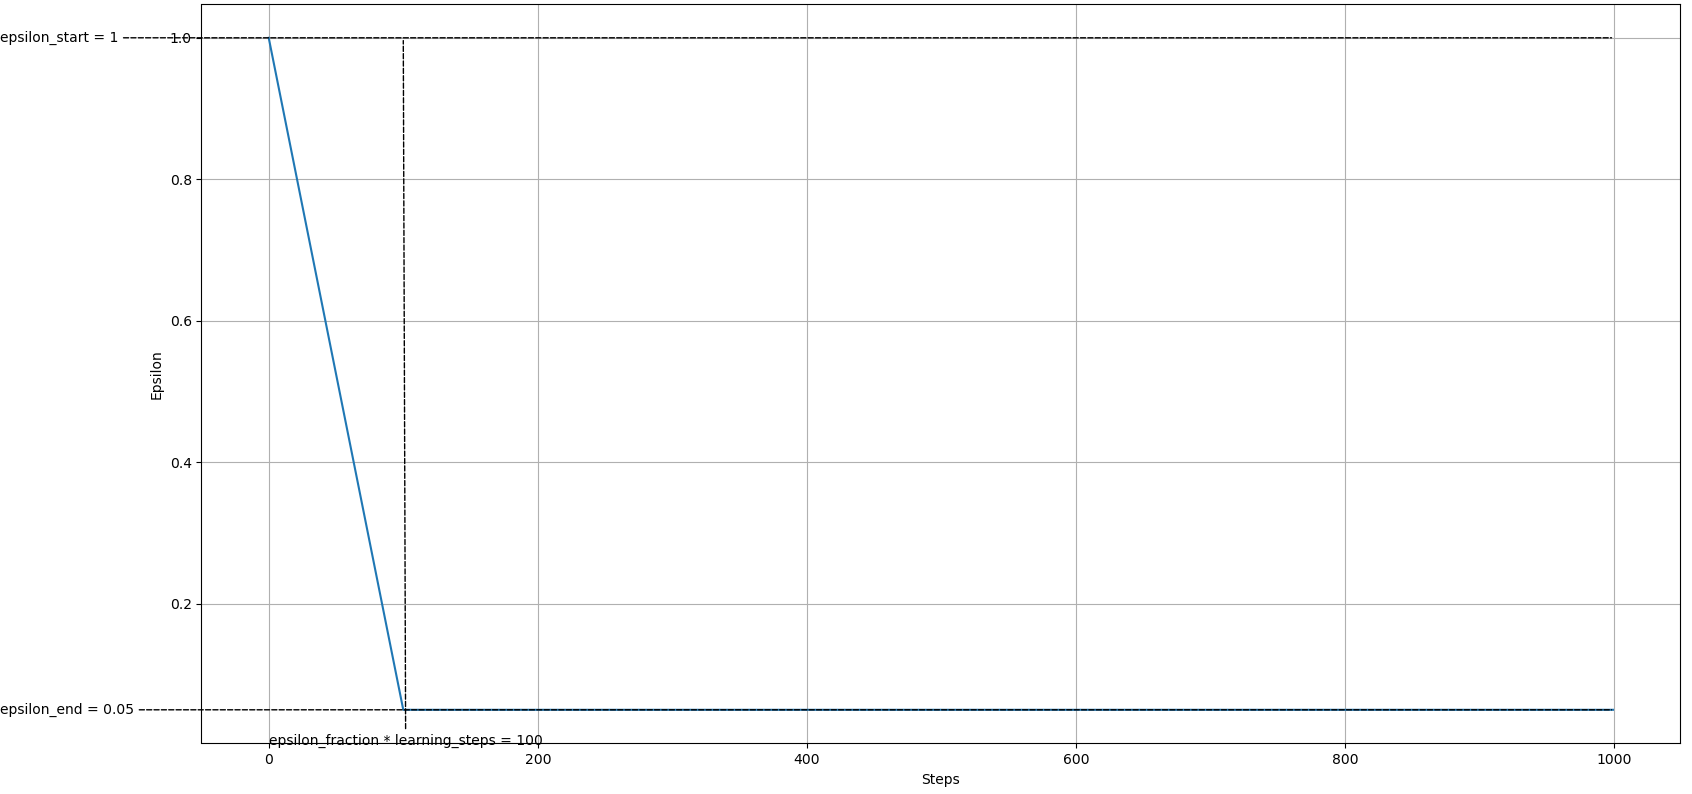
\includegraphics[width=1.1\textwidth]{images/epsilon_decay_2.png}
    \caption{کاهش نرخ کاوش تصادفی در طی آموزش}\label{fig:epsilon_decay}
\end{figure}
\subsection{پیاده‌سازی سایر الگوریتم‌ها به کمک کتابخانه}
یکی از مهم‌ترین مزایای پیاده‌سازی رابط استاندارد جیم، ایجاد امکان استفاده از پیاده‌سازی‌ها و کتاب‌خانه‌های از‌پیش‌موجودی اند که وجود دارند.
با توجه به اینکه اکثر الگوریتم‌های یادگیری تقویتی در کتاب‌خانه‌هایی مانند \lr{Stable Baselines} و \lr{OpenAI Baselines} پیاده‌سازی شده‌اند،
می‌توان از این کتاب‌خانه‌ها برای آموزش عامل‌ها استفاده کرد.
در این پروژه، از کتاب‌خانه \lr{Stable Baselines} برای آموزش عامل‌ها استفاده شده‌است.
کافی‌ست ابتدا یک محیط جدید از جیم تعریف کنیم، مدلی از الگوریتم دلخواه بسازیم، و سپس با استفاده از تابع \lr{learn}
مدل را به تعداد گام‌های دلخواه آموزش دهیم.
\begin{figure}[H]
    \centering
    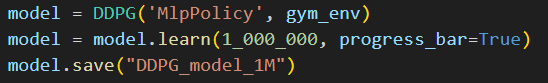
\includegraphics[width=0.75\textwidth]{images/sb3.png}
    \caption{استفاده از کتاب‌خانه \lr{Stable Baselines 3}}\label{fig:sb3}
\end{figure}
طبق مستندات این کتاب‌خانه، می‌توان به مدل توابعی را به عنوان ورودی داد تا در حین آموزش به صورت مکرر و پس از تعداد گام دلخواه به صورت تناوبی صدا زده‌شوند.
 از این توابع می‌توان برای ارزیابی مدل به صورت تناوبی، و ذخیره‌سازی در حین آموزش استفاده کرد که برای مقایسات فصل بعدی بسیار کاربردی است.
\section{جمع‌بندی}
در این فصل، مروری بر راه‌های مختلفی که می‌توان از آن‌ها برای پیاده‌سازی یادگیری تقویتی استفاده کرد، داشتیم.
از جمله این روش‌ها، استفاده از \lr{HFO} و \lr{Pyrus} بودند.
سپس با معرفی پلتفرم جیم، نحوه پیاده‌سازی محیط‌های جدید و تعریف فضای حالت و عمل را مورد بررسی قرار دادیم.

در ادامه، نحوه ادغام این محیط‌ها با فضای ربوکاپ و پیاده‌سازی یک محیط جدید به نام پنالتی را مورد بررسی قرار دادیم.
سپس نحوه پیاده‌سازی یک عامل یادگیری تقویتی با استفاده از شبکه کیو عمیق و کتاب‌خانه \lr{Stable Baselines} را بررسی کردیم.
در فصل بعدی، نتایج این پیاده‌سازی‌ها را مورد بررسی قرار می‌دهیم.
\chapter{مقایسه، آزمایش‌ها، و نتایج}
در این فصل به بررسی نتایج حاصل از پیاده‌سازی الگوریتم‌ها و مقایسه آن‌ها می‌پردازیم.
\section{فرآیند آزمایش}
برای آزمایش، ابتدا الگوریتم‌های معرفی‌ شده در فصل‌های قبل را با یک میلیون گام علیه دروازه‌بان کد پایه \lr{Agent}
آموزش می‌دهیم، و نمودار‌های فرآیند یادگیری را بررسی می‌کنیم. در هر ۵۰۰۰ گام از آموزش مدل به صورت تناوبی ذخیره می‌شود، و در نهایت بهترین مدل‌ها را انتخاب می‌کنیم.
لازم به ذکر است که منظور از گام، گام‌های یادگیری تقویتی است، که هرکدام متناظر با یک ضربه به توپ اند و منظور گام‌های شبیه‌ساز فوتبال نیست.

در نهایت مدل انتخاب شده را برای ۱۰۰ ضربه پنالتی علیه کد پایه قرار می‌دهیم تا با سیاست حریصانه و بدون تصمیم‌گیری تصادفی سنجیده شود، و درصد وقوع هر یک از حالت‌های پایانی بازی را بررسی می‌کنیم.
در نهایت راهکار‌های متفاوتی را برای بهبود نتایج یادگیری امتحان می‌کنیم.

تمامی آزمایش‌ها روی یک سیستم با پردازنده‌ی \lr{AMD Ryzen 7 6800H}، 
حافظه ۳۲ گیگابایت،
و کارت گرافیک \lr{NVIDIA RTX 3070Ti} انجام شده است، 
همراه‌ با کتاب‌خانه‌های کودا 
\LTRfootnote{CUDA}
\lr{CUDA 12.4}, \lr{cudnn 8.9.2}، و \lr{cublas 12.1.3}
انجام شده‌است.
\section{ارزیابی الگوریتم‌ها}
در ابتدا الگوریتم \lr{DQN} را برای یادگیری از صفر امتحان می‌کنیم.
بعد از یک میلیون گام آموزش که حدود ۱۲ ساعت طول کشید، عامل موفق به کشف تکنیک گل زدن نشد.
فرآیند آموزش ۵ بار و با ابرپارامتر‌های متفاوت آزمایش شد، اما در هیچ یک از اجرا‌ها عامل موفق به یادگیری نشد.
یکی از دلایل ممکن این موضوع، می‌توانست تفاوت زیاد بین پاداش‌های موفق و ناموفق باشد، چرا که این موضوع ابعاد گرادیان را بزرگ کرده و باعث عدم ثبات می‌شود. به همین منظور یک ضریب مقیاس‌گر 
برای پاداش‌ها اضافه شد، که باز هم موثر در موفقیت نبود.

\begin{figure}[H]
    \centering
    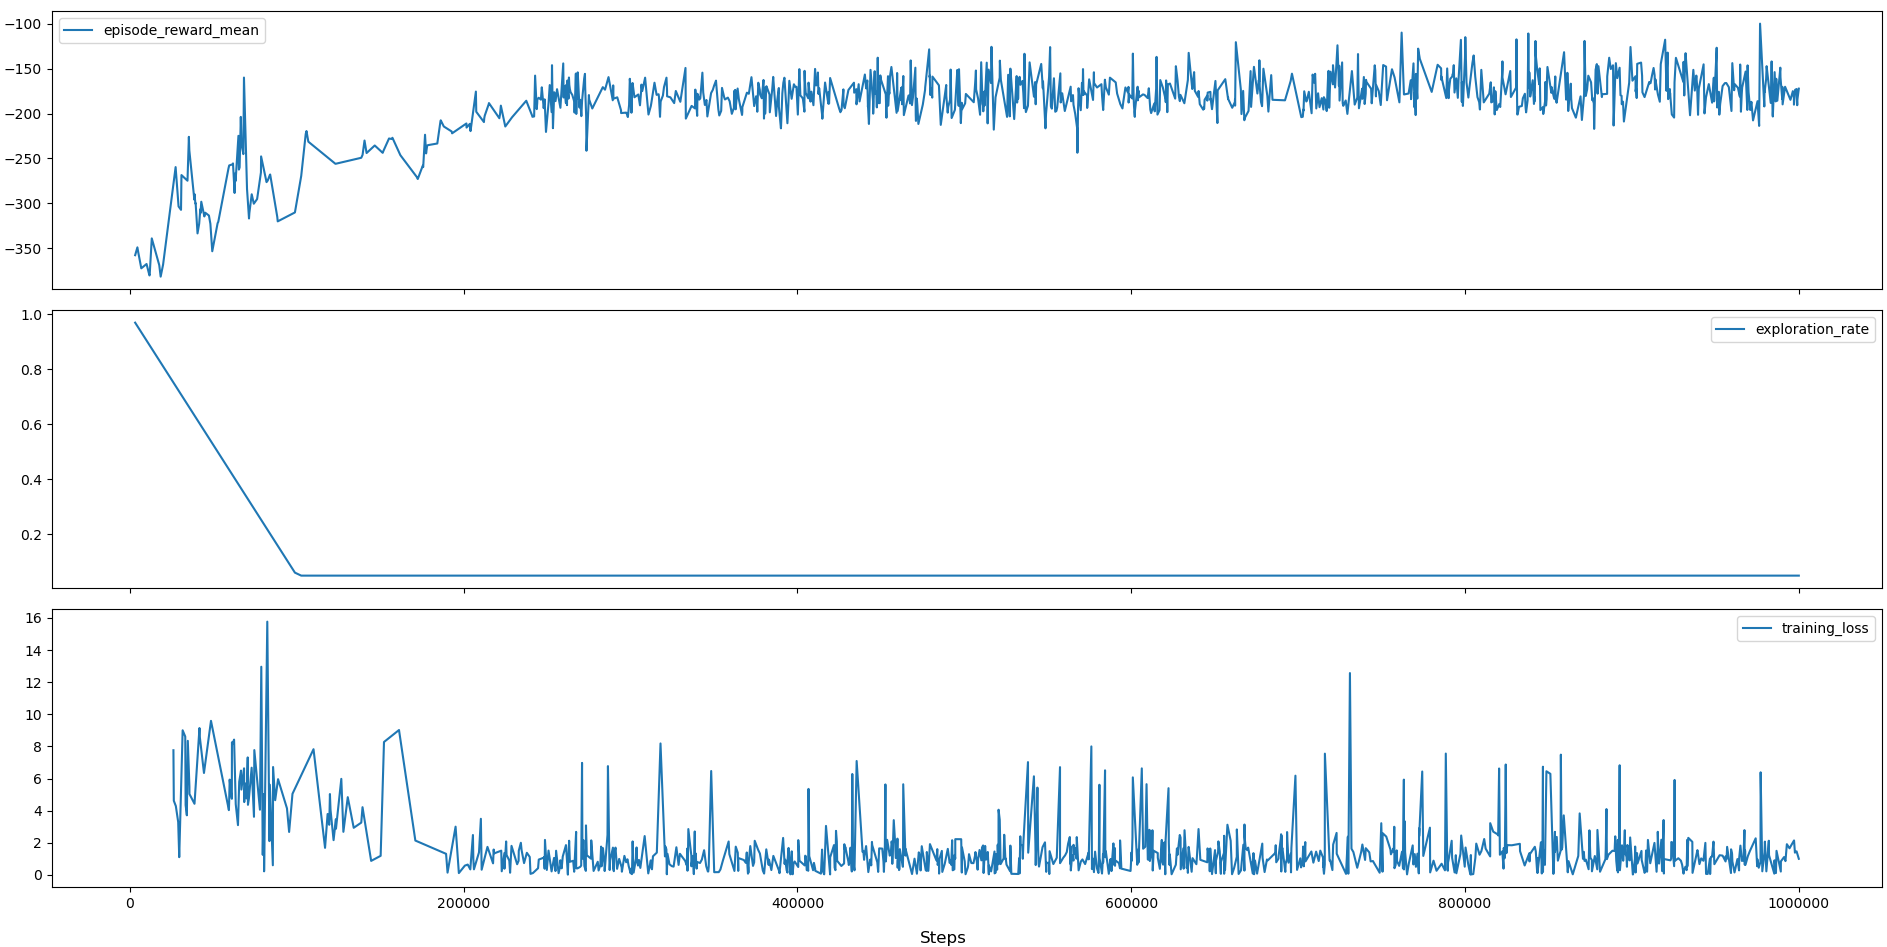
\includegraphics[width=1\textwidth]{images/DQN_graphs.png}
    \caption{نمودار سه پارامتر متفاوت برای یک اجرای الگوریتم \lr{DQN}}\label{fig:dqn_graphs}
\end{figure}

در شکل \ref{fig:dqn_graphs}
می‌توان به ترتیب میانگین پاداش عامل، نرخ کاوش، و خطای شبکه عصبی را در طی زمان آموزش دید.
محور افقی این نمودار گام‌های آموزش است، که در اینجا ۱ میلیون گام است.
مقیاس پاداش‌ها برای این اجرا، ۰.۲
بوده‌است و برای رسم نمودار، به مقیاس ۱ تبدیل شده‌است.
همانطور که می‌توان مشاهده کرد، نمودار خطای شبکه از گام ۵۰۰۰۰ آغاز شده. این به این علت است که آموزش شبکه این گام آغاز می‌شود، تا پیش از آن بافر با حالت‌های متفاوت پر شود.

همانطور که قابل مشاهده است، پاداش‌ها نسبت به حالت آغازین افزایش می‌یابند اما عامل موفق به کشف حالت گل زدن نشده‌است.
میزان خطای شبکه عصبی نیز در طول زمان کاهش یافته و نزدیک به ۱ شده، اما این هم نشان‌دهنده‌ی یادگیری موفق نیست، بلکه شبکه همواره (به درستی)
میزان ارزش حالت شکست را خروجی می‌دهد.

همین فرآیند را با الگوریتم \lr{DDPG} تکرار می‌کنیم.
می‌توان مشاهده کرد که عامل در زیر ۱۰۰ هزار گام موفق به کشف تکنیک گل زدن شده‌است.
همچنین همانطور که در فصل‌های قبلی ذکر شد، به علت محدود بودن اندازه بافر، عامل ممکن است یادگیری خود را فراموش کند.

\begin{figure}[H]
    \centering
    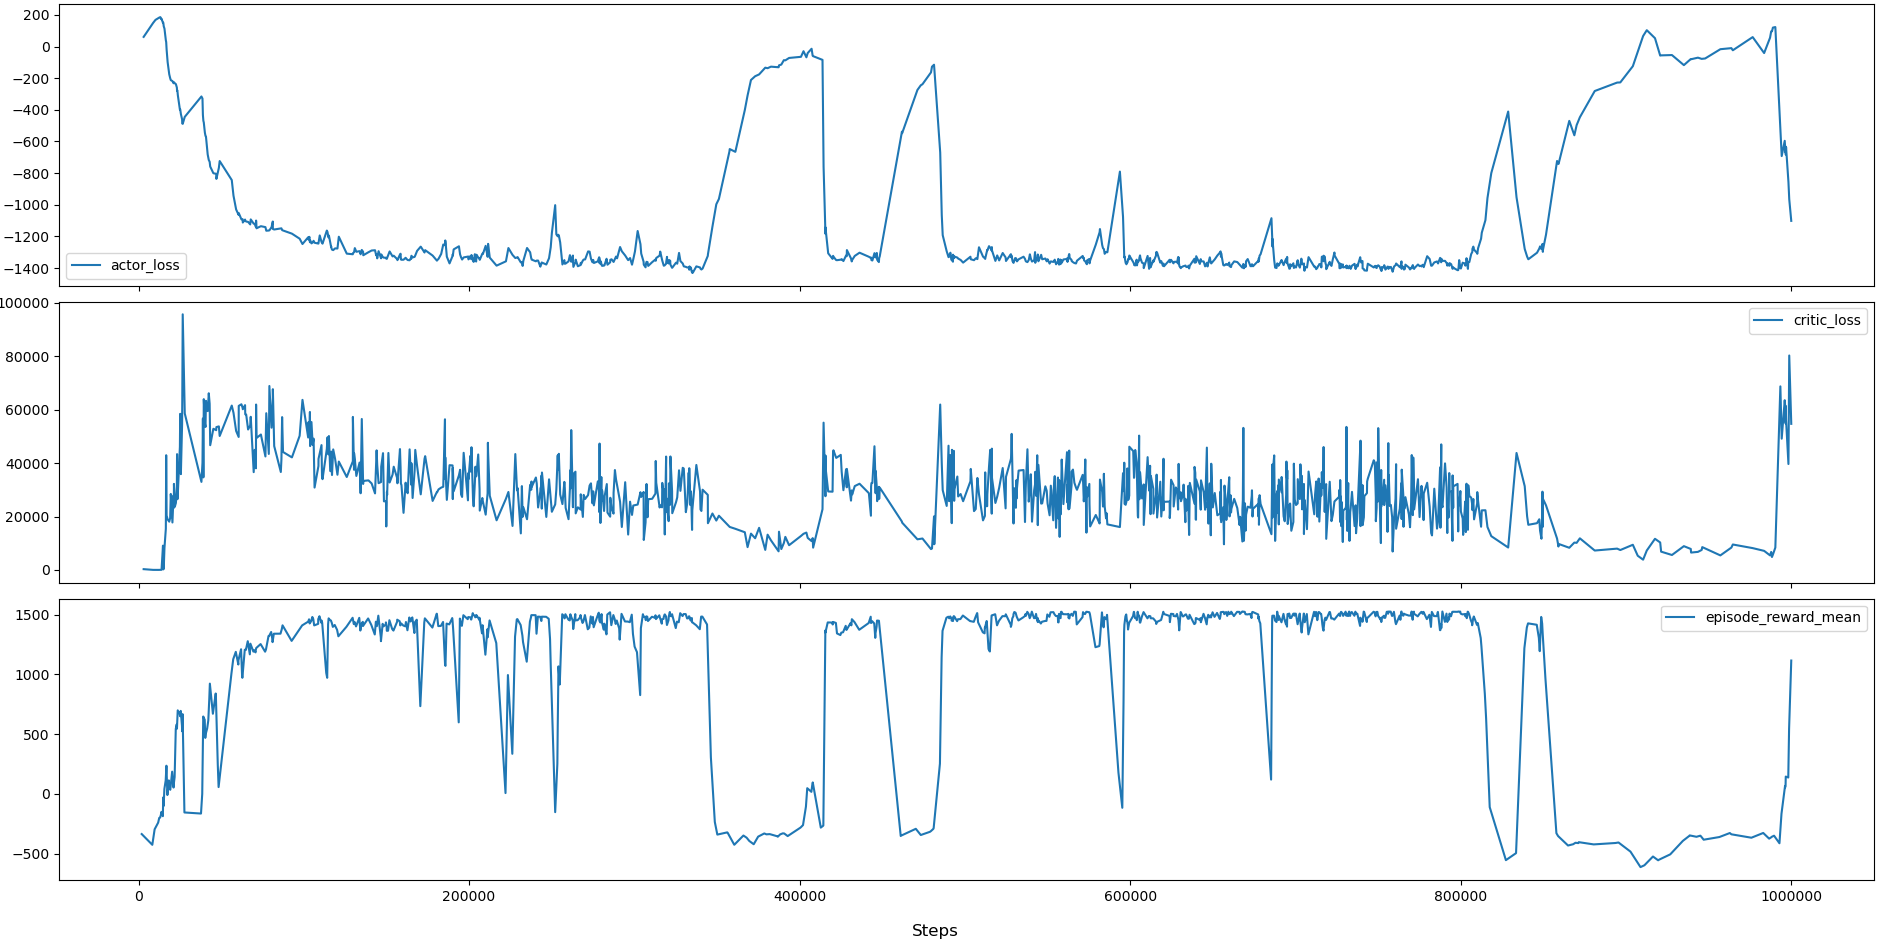
\includegraphics[width=1\textwidth]{images/DDPG_graphs.png}
    \caption{نمودار سه پارامتر متفاوت برای یک اجرای الگوریتم \lr{DDPG}}\label{fig:ddpg_graphs}
\end{figure}

در شکل \ref{fig:ddpg_graphs}
می‌توان به ترتیب خطای شبکه بازیگر، خطای شبکه منتقد، و میانگین پاداش عامل را در طی زمان آموزش دید.
همانطور که می‌توان مشاهده کرد، در حین موفقیت عامل خطای شبکه‌ها و به ویژه خطای بازیگر کاهش یافته‌است.

\begin{table}[H]
    \centering
    \caption{بهترین نتایج الگوریتم‌ها مقابل کد پایه \lr{Agent2D} برای صد پنالتی.}
    \begin{tabular}{ |p{4cm}|p{2cm}|p{2cm}|  }
        \hline
        خروجی & \lr{DQN} & \lr{DDPG} \\
        \hline
        گل زدن & ۲ & ۹۹\\
        \hline
        بیرون رفتن توپ & ۱۸ & ۰\\
        \hline
        گرفتن توسط دروازه‌بان & ۷۴ & ۱\\
        \hline
        اتمام زمان & ۶ & ۰\\
        \hline
        \end{tabular}
        \label{tab:base_results}
\end{table}

با توجه به اینکه الگوریتم \lr{DDPG} موفق بود، می‌توان حدس‌هایی راجع به عدم موفقیت \lr{DQN} زد.
یکی از دلایل، این است که به علت گسسته بودن اعمال، تعداد گام‌های لازم برای رسیدن به گل بیشتر است، و از آنجا که عامل باید به صورت تصادفی گل زدن را کشف کند،
عامل به تعداد دفعات کافی به این حالت نمی‌رسد.
همچنین همانطور که در شکل \ref{fig:actor_critic} می‌توان دید، شبکه در الگوریتم
\lr{DQN} به ازای هر عمل، یک خروجی دارد و به همین علت، فضای عمل بزرگ یادگیری را به مراتب دشوار می‌کند.
از این رو می‌توان سه راه را برای بهبود یادگیری این الگوریتم پیشنهاد داد:
\begin{enumerate}
    \item بهبود گسسته‌سازی عمل‌ها.
    \item استفاده از پاداش های بهتر برای حالت‌های غیرنهایی که عامل را به سمت حالت‌های مفید‌تر هدایت کند.
    \item تغییر فضای عمل و جدا‌سازی اعمال به دریبل‌ زدن و شوت زدن.
\end{enumerate}

\section{بهبود تابع پاداش}
برای بهبود تابع پاداش، به روش گل‌زنی الگوریتم \lr{DDPG} نگاه می‌کنیم.
به نظر می‌آید که نزدیک شدن دروازه‌بان به توپ عامل منفیی نیست، چرا که این حالت ممکن است به عامل کمک کند تا با یک ضربه به توپ، زاویه دروازه را باز کند.
همچنین در صورت نزدیکی بیش از حد دروازه‌بان به توپ در حین ضربه، عامل می‌تواند از قابلیت گسسته بودن زمان شبیه‌ساز استفاده کند و با انجام قوی‌ترین ضربه ممکن، توپ را از روی دروازه‌بان بگذراند.
بنابرین برای گام‌های بعدی، عامل فاصله با دروازه‌بان را از محاسبات پاداش حذف می‌کنیم.


\section{جدا‌سازی عمل شوت}
عامل در ابتدای یادگیری، هنوز به درک اینکه در چه حالتی می‌تواند شوت منجر به گل داشته باشد نرسیده است.
از آنجا که این عمل با عمل رسیدن به موقعیت شوت‌زنی متفاوت است، عامل ممکن است دیر به دیر به حالت‌هایی که شوت زدن در آن ممکن است برسد.
بنابرین در حین یادگیری نسبت به ضربه با سرعت‌های بالا بدبین می‌شود.

برای حل این مشکل، فضای عمل را به گونه‌ای اصلاح می‌کنیم که شوت زدن جدا باشد.
\subsection{شوت با رفتار سطح بالای کد پایه}
یک عمل خاص مدنظر می‌گیریم که در صورت انتخاب شدن توسط عامل، شوت کد پایه \lr{Agent2D} 
انجام می‌شود. این کد در صورت وجود شوت ممکن، آن را انجام می‌دهد و در غیر این صورت، هیچ عملی انجام نمی‌شود.
در صورتی که عامل این عمل را انتخاب کند ولی به گل نرسد، پاداش منفیی به آن داده می‌شود، تا عامل استفاده صحیح از این ابزار را یاد بگیرد.
\begin{figure}[H]
    \centering
    \begin{tikzpicture}
        \pie[rotate=90, color={green, red, orange, yellow}]
        {
            3/گل,
            12/توپ رفتن بیرون,
            49/دروازه‌بان توسط گرفتن,
            36/زمان اتمام
        }
    \end{tikzpicture}
    \caption{نتیجه ۱۰۰ ضربه پنالتی با شوت سطح بالا مقابل کد پایه \lr{Agent2D} برای عامل یادگیری‌شده}\label{fig:helios_shoot_pie}
\end{figure}

طبق تجربه پیش از این پروژه، این رفتار سطح بالا بسیار محافظ‌کارانه تصمیم می‌گیرد.
از این رو شاید کمک چندانی به عامل برای یادگیری نکند.
همچنین از آنجا که استفاده از این قابلیت بسیار وابسته به شبیه‌سازی ضربه به توپ و بررسی امکان قطع توپ توسط دروازه‌بان است، خلاف ماهیت انجام این پروژه است.
\subsection{عمل شوت به نقاط ثابت دروازه}
فرض کنید تعدادی نقطه ثابت دروازه را انتخاب کنیم.
هر یک از این نقاط متناظر با یک عمل شوت است.
در این عمل، به توپ با حداکثر سرعت ممکن در راستای این عمل ضربه می‌زنیم.
برای انتخاب نقاط، دو تیرک دروازه را به عنوان نقاط ثابت در نظر گرفته، و فضای بین این نقطه را به $n-1$ نقطه تقسیم می‌کنیم.
\begin{figure}[H]
    \centering
    \begin{tikzpicture}
        \pie[rotate=90, color={green, red, orange, yellow}]
        {
            19/گل,
            4/توپ رفتن بیرون,
            53/دروازه‌بان توسط گرفتن,
            24/زمان اتمام
        }
    \end{tikzpicture}
    \caption{نتیجه تست ۱۰۰ پنالتی مقابل کد پایه \lr{Agent2D} با ۵ نقطه شوت.}\label{fig:custom_shoot_pie}
\end{figure}

\section{تغییر گسسته‌سازی}
حال که عامل دارای عمل مستقیم شوت است، می‌توانیم گسسته‌سازی قدرت را به گونه‌ای تغییر دهیم که سرعت‌های بالا را نداشته باشد.
برای این منظور ضربه به توپ را به سه سرعت تقسیم می‌کنیم: ۱۵ درصد حداکثر سرعت توپ، ۲۵ درصد حداکثر سرعت توپ، و ۵۰ درصد حداکثر سرعت توپ.
در واقع اعمال ممکن را به شوت به نقطه یا دریبل با سرعت و زاویه معین تقسیم می‌کنیم.

همچنین به صورت شهودی می‌توان برداشت کرد که تقسیم زوایای جلوی بازیکن به شدت مهم‌تر از زوایای پشت بازیکن است، 
چرا که به ندرت نیاز می‌شود بازیکن با ضربه به عقب پیشرفت کند.
زوایای جلوی بازیکن را به ۹ قسمت تقسیم می‌کنیم، و دو راستا برای دریبل به عقب (بالا عقب و پایین عقب) اضافه می‌کنیم.

با ترکیب این دو تکنیک، فضای حالت از ۱۲۰ عمل، به ۳۸ عمل کاهش می‌یابد.
این کاهش از دو راستا به یادگیری ما کمک می‌کند:
\begin{itemize}
    \item کاهش ابعاد گرادیان و افزایش سرعت یادگیری
    \item افزایش احتمال انجام عمل مفید به کمک کاوش، به علت حذف رفتار‌هایی که به احتمال زیاد مفید نیستند
\end{itemize}
پس از یک میلیون گام آموزش، نمودار پاداش‌ها و درصد موفقیت در حین آموزش را مشاهده می‌کنیم.
\begin{figure}[H]
    \centering
    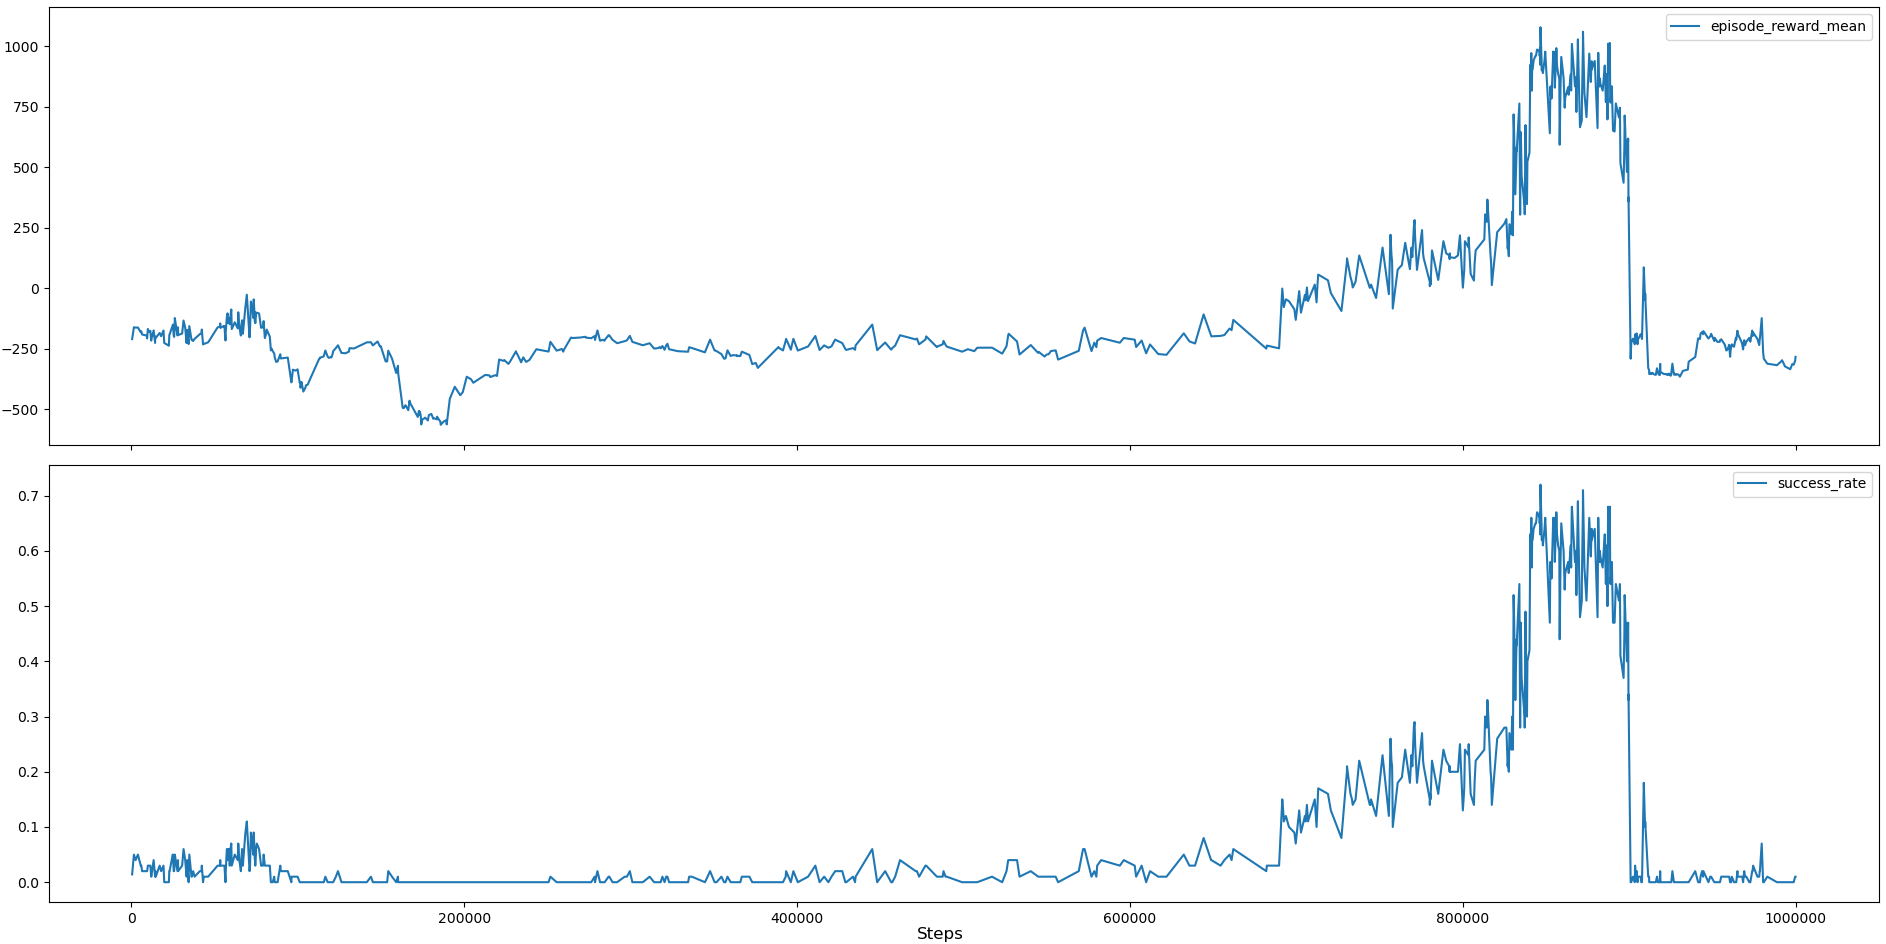
\includegraphics[width=1\textwidth]{images/dqn_discretization.png}
    \caption{نمودار میانگین نرخ گل‌زنی و میانگین پاداش \lr{DQN} با تغییرات گسسته‌سازی}\label{fig:discretization_change}
\end{figure}
همانطور که در تصویر مشاهده می‌کنید، با این تغییرات عامل موفق به کشف روش گل‌زنی و موفقیت ۷۲ درصد شده‌است.
همچنین می‌توان دید که نمودار پاداش و نرخ گل‌زنی هم‌رفتار و تقریبا هم‌شکل هستند.
\begin{figure}[H]
    \centering
    \begin{tikzpicture}
        \pie[rotate=90, color={green, red, orange, yellow}]
        {
            74/گل,
            2/توپ رفتن بیرون,
            24/دروازه‌بان توسط گرفتن,
            0/زمان اتمام
        }
    \end{tikzpicture}
    \caption{نتیجه تست ۱۰۰ پنالتی مقابل کد پایه \lr{Agent2D} با ۵ نقطه شوت.}\label{fig:discretization_pie}
\end{figure}

\section{بررسی تعمیم پذیری}
در این بخش، با تست علیه دروازه‌بان تیم‌هایی که مقابل آن‌ها یادگیری رخ نداده، می‌بینیم که آیا این یادگیری تعمیم‌پذیر بوده یا خیر.
با توجه به اینکه پس از مسابقات، فایل‌های اجرایی تیم‌ها در اختیار سایر شرکت‌کنندگان قرار می‌گیرد، می‌توانیم این تست را انجام دهیم.
از ۳ تیم برای این منظور استفاده می‌کنیم:
تیم 
\lr{Helios2023}
 که قهرمان پیاپی چندین دوره است، تیم کد پایه \lr{Agent2D}
 که مبنای بسیاری از سایر تیم‌ها است،
تیم \lr{YuShan2023} که از تیم‌های موفق دیگر است و استراتژی متفاوتی نسبت به دو تیم قبلی دارد.

\begin{table}[H]
    \centering
    \caption{نتایج تست الگوریتم \lr{DDPG} علیه تیم‌های مختلف}\label{tab:generalization}
        \begin{tabular}{ |p{4cm}|p{2cm}|p{2cm}|p{2cm}|  }
            \hline
            خروجی & \lr{Agent2D} & \lr{Helios2023} & \lr{YuShan2023}\\
            \hline
            گل زدن & ۹۹ & ۴۰ & ۲۷ \\
            \hline
            بیرون رفتن توپ & ۰ &۴ & ۱۱ \\
            \hline
            گرفتن توسط دروازه‌بان & ۱ &۴۰ & ۵۷ \\
            \hline
            اتمام زمان & ۰ &۱۶ & ۴ \\
            \hline
        \end{tabular}
\end{table}
به صورتی شهودی و دیدن نتایج تست، می‌توان دید که نتایج تا حدودی قابل تعمیم است، اما شوت زدن عامل بسیار وابسته به مختصات دروازه‌بان است و از این رو، شوت‌های به بیرون و یا گرفته شده توسط دروازه‌بان افزایش یافته‌اند.
همچنین دروازه‌بان سایر تیم‌ها مانند \lr{Helios2023}،
 در شرایطی که نتوانند به توپ برسند از دستور تکل استفاده می‌کنند، که برد بیشتری نسبت به گرفتن توپ دارد ولی به صورت احتمالاتی است. در صورت تکل موفق حالت گرفتن توسط دروازه‌بان ثبت می‌شود.

\begin{table}[H]
    \centering
    \caption{نتایج تست الگوریتم \lr{DQN} بهبود یافته مقابل تیم‌های مختلف}\label{tab:dqn_generalization}
        \begin{tabular}{ |p{4cm}|p{2cm}|p{2cm}|p{2cm}|  }
            \hline
            خروجی & \lr{Agent2D} & \lr{Helios2023} & \lr{YuShan2023}\\
            \hline
            گل زدن & ۷۱ & ۰ & ۱۰ \\
            \hline
            بیرون رفتن توپ & ۰ &۰ & ۱۵ \\
            \hline
            گرفتن توسط دروازه‌بان & ۲۹ &۱۰۰ & ۷۰ \\
            \hline
            اتمام زمان & ۰ &۰ & ۵ \\
            \hline
        \end{tabular}
\end{table}
با توجه به گسسته‌سازی، هر گونه تغییر در موقعیت دروازه‌بان عمل بعدی عامل را به شدت تحت تاثیر قرار می‌دهد و عامل به شدت با حالت‌های از پیش دیده فاصله می‌گیرد.
از این رو همانطور که پیش‌بینی می‌شد، تعمیم‌پذیری این الگوریتم به تیم‌های دیگر بسیار پایین است.

در نهایت یادگیری الگوریتم \lr{DDPG} را تکرار می‌کنیم، با این تفاوت که آموزش را از ابتدا و مقابل تیم‌های مختلف انجام می‌دهیم.
این آزمایش از این رو است که ببینیم در صورتی که آموزش روی تیم‌های قوی‌تر انجام شود، آیا عامل موفق به یادگیری تکنیک‌های مفید‌تری می‌شود یا خیر.

فرآیند آموزش تا زمانی ادامه می‌یابد که عامل به تکنیک گل‌زنی مقابل تیم آموزشی برسد، و تا یک میلیون گام ادامه نخواهد یافت.
برای یادگیری مقابل تیم \lr{Helios2023} فقط ۱۵۰ هزار گام کافی بود تا نرخ موفقیت به بالا ۹۰ درصد برسد که حدود یک ساعت زمان برد. یادگیری مقابل تیم \lr{YuShan2023}  حدود ۷۰ هزار گام طول کشید که ۲۰ دقیقه زمان برد.


\begin{table}[H]
    \centering
    \caption{نتایج تست الگوریتم \lr{DDPG} علیه تیم‌های مختلف با آموزش مقابل تیم \lr{Helios2023}}\label{tab:ddpg_helios_generalization}
        \begin{tabular}{ |p{4cm}|p{2cm}|p{2cm}|p{2cm}|  }
            \hline
            خروجی & \lr{Agent2D} & \lr{Helios2023} & \lr{YuShan2023}\\
            \hline
            گل زدن & ۴۷ & ۹۰ & ۲۳ \\
            \hline
            بیرون رفتن توپ & ۱۶ &۰ & ۵ \\
            \hline
            گرفتن توسط دروازه‌بان & ۳۷ &۷ & ۶۵ \\
            \hline
            اتمام زمان & ۰ &۳ & ۷ \\
            \hline
        \end{tabular}
\end{table}

\begin{table}[H]
    \centering
    \caption{نتایج تست الگوریتم \lr{DDPG} علیه تیم‌های مختلف با آموزش مقابل تیم \lr{YuShan2023}}\label{tab:ddpg_yushan_generalization}
        \begin{tabular}{ |p{4cm}|p{2cm}|p{2cm}|p{2cm}|  }
            \hline
            خروجی & \lr{Agent2D} & \lr{Helios2023} & \lr{YuShan2023}\\
            \hline
            گل زدن & ۰ & ۰ & ۹۹ \\
            \hline
            بیرون رفتن توپ & ۰ &۰ & ۰ \\
            \hline
            گرفتن توسط دروازه‌بان & ۸۳ &۱۰۰ & ۱ \\
            \hline
            اتمام زمان & ۱۷ &۰ & ۰ \\
            \hline
        \end{tabular}
\end{table}

به نظر می‌رسد که استراتژی متفاوت \lr{YuShan2023} باعث می‌شود عامل‌هایی که روی سایر تیم‌ها آموزش دیده‌اند گیج شوند و نتوانند به موفقیت برسند.
اما آموزش روی \lr{YuShan2023} که به دور زدن دروازه‌بان در آن آسان‌تر است، باعث می‌شود که عامل 
به موفقیت جلوی سایر تیم‌ها نرسد، چرا که تاکتیک موفق جلوی \lr{YuShan2023} منجر به گرفتن توسط دروازه‌بان می‌شود.

از سوی دیگر، با توجه به این که استراتژی \lr{Helios2023} مشابه ولی قوی‌تر نسبت به \lr{Agent2D} است، آموزش مقابل آن باعث می‌شود که عامل به موفقیت نسبی نزدیک شود.

لازم به ذکر است که حتی اگر عامل در دو دور آموزش مقابل تیم آموزشی به نتایج یکسان برسد، نمی‌توان انتظار داشت که نتایج تست مقابل سایر تیم‌ها یکسان باشد. به این منظور که اگر آموزش را دو بار از صفر آغاز کنیم و تا صد درصد موفقیت پیش ببریم، ممکن است نتایج تست مقابل تیم‌های دیگر بین دو حالت نزدیک نباشد. از این رو این آزمایش معیار خیلی دقیقی برای بررسی کمی تعمیم‌پذیری نیست.

در آینده می‌توان راه‌های تولید مدل‌های تعمیم‌پذیر‌تر را بیشتر بررسی کرد. یکی از این راه‌ها استفاده از حریف‌های متفاوت در حین یادگیری، و روش‌های یادگیری تقویتی مداوم\LTRfootnote{Continual Reinforcement Learning} است.

\section{جمع‌بندی}
در این فصل، ما الگوریتم‌های یادگیری تقویتی \lr{DQN} و \lr{DDPG} را برای یادگیری تکنیک گل‌زنی در فوتبال تک به تک مورد بررسی قرار دادیم.
همچنین چند راه حل برای بهبود یادگیری این الگوریتم‌ها ارائه دادیم.
در نهایت، تعمیم‌پذیری این الگوریتم‌ها را بررسی کردیم و دیدیم که طبق توقع، عامل در مقابل حریف‌هایی که از پیش ندیده، قدرت یادگیری کمتری دارد.

%%%%%%%%%%%%%%%%%%%%%%%%%%%%%%%%%%%%%%%%%%%
% در بخش پایانی گزارش، جمعبندي و مروري بر سیر مطالب عنوان شده در گزارش خواهیم داشت. همچنین نتایج حاصل را بیان
% کرده و پیشنهادهایی براي ادامه کار در این موضوع ارائه میدهیم.
% \section{نتیجه‌گیری}
% این گزارش ۶ الگوریتم‌ برای پیش‌بینی مصرف انرژی ساختمان‌ها را مورد بررسی قرار داد که برای این الگوریتم‌ها داده‌های مصرف آینده‌ی ساختمان‌ها و مصرف گذشته‌شان موجود بود. 
% همچنین در این مقاله اهمیت برخی متغیرها مانند وضعیت دمای محیط و تعداد ساکنین ساختمان در هر زمان نیز مورد توجه قرار گرفتند و اهمیت آن‌ها در تصمیم گیری مشخص گردید.
% چندین مدل یادگیری ماشین موفق با استفاده از داده‌های انرژی ثبت‌شده گذشته برای پیش‌بینی کوتاه‌مدت، میان‌مدت و بلندمدت توسعه یافته‌اند. مشاهده می شود 
% که هر یک از تکنیک های توصیف شده دارای مجموعه ای از مزایا و معایب است. اینها با توجه به تجزیه و تحلیل داده های انرژی ساختمان به تفصیل تجزیه و تحلیل و ارائه شده اند.
%  تأکید ویژه بر مدل ترکیبی داده شده است، که ترکیبی از دو یا چند تکنیک یادگیری ماشینی است به نحوی که هر مدل قدرت دیگری 
%  را تحسین می کند. به عنوان مثال، یک مدل ترکیبی که میانگین متحرک خودهمبسته یکپارچه و الگوریتم‌های تکاملی را در نظر می‌گیرد، می‌تواند
%   از مدل میانگین متحرک خودهمبسته یکپارچه برای تعیین تناوب و خطی بودن استفاده کند، در حالی که الگوریتم‌ تکاملی می‌تواند به طور موثر باقیمانده‌ها را تعیین کند. ترکیبات مختلفی از مدل ترکیبی و تازگی آنها در
%    ادبیات شناسایی شده و به طور سیستماتیک در این مقاله ارائه شده است. مشاهده می‌شود
%    که ترکیب تکنیک‌های پیش‌بینی سری‌های زمانی مانند شبکه ی عصبی مصنوعی، میانگین متحرک خودهمبسته یکپارچه به خوبی با 
%    تکنیک‌های بهینه‌سازی ترکیب می‌شوند. چنین ترکیب‌هایی به طور گسترده در تحقیقات اختصاص یافته به بهینه‌سازی ساختمان مورد بررسی قرار گرفته‌اند.
%     انتظار می رود روند رو به رشد
%     در تحقیقات در بهره وری انرژی ساختمان در پرتو انگیزه پایداری جهانی ادامه یابد. این امر نظارت و پیش بینی داده های انرژی در 
%     زمان واقعی را در این زمینه مرتبط و حیاتی می کند. این مقاله خلاصه‌ای جامع از تکنیک‌های پیش‌بینی موجود همراه با ترکیبی
%      از مدل ترکیبی ارائه می‌کند و راه را برای تحقیقات آینده در زمینه مصرف انرژی ساختمان هموار می‌کند.
%      \\
%      حوزه بهینه سازی ساختمان بر اساس یک شبکه گسترده جمع آوری داده، نظارت، پیش بینی، بهینه سازی و کنترل است. تمام این زیرساخت‌ها
%       همواره به کل هزینه عملیاتی ساختمان می‌افزایند. چالش در اینجا بررسی مزایای اضافه شده از نظر هزینه سرمایه گذاری و هزینه به دست آمده
%       به دلیل صرفه جویی در انرژی ناشی از بهینه سازی ساختمان است. مطالعات کمی وجود دارد که بخش مالی را برای کنترل عملکرد و بهینه سازی ساختمان 
%      برجسته می کند. این محدودیت در به اشتراک گذاری داده های هزینه یا به دلیل 
%      نیروهای بازار درگیر است یا به دلیل محرمانه بودن ماهیت داده های درگیر. لبی الدان\LTRfootnote{Labeodan} 
%      و همکاران. کاربردهای شبکه حسگرها و محرک‌های بی‌سیم کم‌هزینه را برای مدل‌سازی اشغال و کنترل روشنایی در یک ساختمان
%       اداری مورد بحث قرار داد \cite{labeodan2016application}. هزینه کل سیستم تقریبا 2575 یورو برای 12 ایستگاه کاری بود که
%       شامل حسگرهای حرکتی بی سیم و سنسورهای صندلی بود. نتایج نشان می دهد که به طور متوسط 24\% کاهش در مصرف انرژی روشنایی برای یک دوره
%       دو هفته ای با هزینه اجرا شده در حدود 215 یورو برای هر ایستگاه کاری است. نویسندگان خاطرنشان کردند که هزینه اولیه بالاتر و عدم آگاهی از عوامل مؤثر
%       در کاهش سرعت استقرار حسگرها هستند. با این حال، صرفه جویی در انرژی به دست آمده، سهولت استقرار و بهبود سنجش محیطی این
%       را به عنوان یک راه حل مناسب برای دستیابی به عملکرد بهبود 
%       یافته ساختمان نشان می دهد. کومار و همکاران همچنین متوجه شد که هزینه سنسورهای نظارت کنترل کیفیت هوای داخلی الزامات استقرار در مقیاس بزرگ برای کنترل و اتوماسیون را
%        برآورده نمی کند \cite{kumar2016real}. لیلیس و همکاران اشاره کنید
%        که علاقه به راه‌حل‌های 
%       مبتنی بر اینترنت اشیا\LTRfootnote{Internet Of Things (IOT)} مدرن برای بهینه‌سازی ساختمان به دلیل عدم برآورد منافع هزینه، مهار شده است \cite{lilis2017towards}. چن و همکاران اشاره کرد
%        که هزینه مربوط به مصرف انرژی مجموعه تصادفی ساختمان‌ها در چین با سیستم های اتوماسیون ساختمان تقریبا دو برابر ساختمان های
%        بدون سیستم اتوماسیون ساختمان است \cite{chen2016cost}. این به دلیل نقص سنسور و نقص استراتژی کنترل است که منجر به افزایش قابل توجهی در مصرف انرژی نهایی می شود.
%         \\
%         چند مطالعه مروری شبکه حسگر بی سیم را پوشش داده است که سیستم مدیریت انرژی ساختمان را برای کاربردهای خانه/ساختمان 
%         هوشمند فعال کرده است \cite{kazmi2014review,kuzlu2015review}. از آنجایی که فناوری کنترل پیش‌بینی مدل هنوز در مرحله توسعه است و 
%         نیاز به بهینه‌سازی سنگین بر اساس نوع و عملکرد ساختمان دارد،
%          پیاده‌سازی در حال حاضر بیشتر بر روی بستر آزمایشی و اعتبارسنجی تمرکز دارد. در عین حال، این فناوری هنوز
%          با هزینه لازم برای استقرار در مقیاس های بزرگ در دسترس نیست. 
%          این چالش ها منجر به نفوذ آهسته اتوماسیون ساختمان و بهینه سازی در کل می شود. دامنه این مقاله مروری، با این حال
%         ، محدود به مطالعه تکنیک‌های پیش‌بینی سری‌های زمانی برای مصرف انرژی ساختمان است که بخشی جدایی‌ناپذیر
%          از فرآیند بهینه‌سازی و کنترل ساختمان است.
% \section{پیشنهادها}
%     به طور کلی الگوریتم‌های هوش‌ مصنوعی که در زمینه‌ی پیش‌بینی سری داده‌های زمانی کار میکنند و بخش عمده‌ی آن‌ها که الگوریتم‌های یادگیری ماشین می‌شوند مشکلات و سختی‌های مخصوصی دارند
%     از جمله محدودیت‌های مربوط به یادگیری‌آن‌ها که نیازمند داده‌های بسیتر زیاد برای یادگیری و آموزش میباشد و هم‌چنین نیاز به توان پردازشی بالای آن‌ها که از جمله مشکلات روش‌های هوش مصنوعی 
%     به طور کلی میباشد. 
%     برای حل این مشکل پیشنهاد میشود که الگوریتم‌های نوینی با استفاده از روش‌های ترکیبی توسعه داده بشوند که نیاز به داده‌های زیاد برای یادگیری در آن‌ها کمتر باشد و بتوانند با شبیه‌سازی 
%     آموزش ببینند و همچنین برای حل مشکل پردازش‌های سنگین با تحقیقات جدید به سمت برخط کردن یادگیری الگوریتم‌های هوش مصنوعی حرکت بکنیم به این صورت که تمام پردازش‌های مورد نیاز 
%     الگوریتممان برروی سرورهای قدرتمندی در سطح منطقه انجام بشوند و ساختمان‌ها مشکل پردازشی‌شان از این نظر مرتفع بشود و تنها برای انجام اندازه‌ی مشخصی از پردازش برروی شبکه ی قدرتمندمان 
%     هزینه پرداخت کنند تا هزینه‌هایشان کاهش پیدا بکند.
\chapter{جمع‌بندی، نتیجه‌گیری و پیشنهادات}
در این فصل مروری بر سیر مطالب عنوان شده خواهیم داشت.
سپس مروری بر نتایج‌ و دستاورد‌های این پروژه خواهیم داشت و در نهایت پیشنهاداتی برای ادامه‌ی کار در این موضوع ارائه خواهیم کرد.
\section{جمع‌بندی و نتیجه‌گیری}
در این پروژه قصد داشتیم تا با استفاده از روش‌های یادگیری تقویتی یک محیط مجازی برای آموزش و تقویت بازیکنان فوتبال ایجاد کنیم.
به این منظور ابتدا با مفاهیم اساسی یادگیری تقویتی آشنا شدیم،
با مهم‌ترین روش‌های پیاده‌سازی کلاسیک آن آشنا شدیم و در نهایت با روش‌های پیشرفته‌تری همچون یادگیری تقویتی عمیق و برخی الگوریتم‌های آن آشنا شدیم.
در دو الگوریتم یادگیری کیو عمیق و یادگیری گرادیان سیاست قطعی عمیق به طور دقیق با فرآیند یادگیری و عوامل موثر در آن آشنا شدیم.

در ادامه محیط شبیه‌ساز دو بعدی فوتبال را معرفی کردیم و برخی از ویژگی‌های آن را توضیح دادیم.
رفتار‌های مجاز بازیکنان را بررسی کردیم، و کمی با تاریخچه ربوکاپ آشنا شدیم. سپس حالت پنالتی را به عنوان یک محیط مناسب برای یادگیری تقویتی معرفی کردیم.
در بخش بعدی تلاش‌های متفاوتی که برای پیاده‌سازی یادگیری تقویتی در شبیه‌سازی فوتبال انجام شده‌بود را بررسی کردیم.
در نهایت رابط استاندارد جیم را معرفی کردیم و یک پیاده‌سازی برای اتصال این رابط با کد پایه شبیه‌ساز به کمک جی‌آر‌پی‌سی انجام دادیم.

در نهایت با استفاده از الگوریتم‌های یادگیری تقویتی عمیق، یک مدل برای آموزش سمت مهاجم در موقعیت‌های تک به تک با دروازه‌بان ایجاد کردیم و الگوریتم‌های متفاوت را مقایسه کرده، و پیشنهاداتی برای بهبود عملکرد آن‌ها ارائه کردیم.
\section{کار‌های آتی}
در آینده می‌توان از زیرساخت ایجاد شده در سه راستا استفاده کرد: حل سایر مسائل در لیگ شبیه‌ساز دو بعدی، استفاده از محیط برای ارزیابی الگوریتم‌ها و روش‌های یادگیری،
و بررسی تاثیر ویژگی‌های مختلف بر عملکرد مدل‌های یادگیری تقویتی.
برخی از پیشنهاداتی که در این زمینه‌ها می‌توان ارائه کرد عبارتند از:
\begin{enumerate}
    \item   بررسی یادگیری تقویتی در حالت‌های چند عامله: یکی از بزرگترین چالش‌های یادگیری تقویتی، یادگیری در حالت‌های چند عامله‌ای است که نیاز به هماهنگی بین عامل‌ها دارد. این زیرساخت و محیط فوتبال می‌تواند محل مناسبی برای توسعه ایده‌های جدید در این راستا باشد.

    یک نمونه از این مسائل انتخاب حریف و یارگیری به صورت مجزا برای هر بازیکن است. از چالش‌های این مسئله می‌توان به مشکل همگام بودن عوامل در تصمیم‌گیری، بزرگی فضای حالت، و تفاوت میان اطلاعات عامل‌ها به دلیل دید ناقص اشاره کرد.
    \item بررسی تغییر روش نمایش ویژگی‌ها و تاثیر آن بر عملکرد مدل‌های یادگیری تقویتی: یکی از مهم‌ترین مسائل در یادگیری تقویتی، انتخاب نمایش مناسب برای ویژگی‌ها است. انتخاب نمایش مناسب می‌تواند تاثیر بزرگی بر عملکرد مدل‌ها داشته باشد.
    به طور مثال، موقعیت بازیکن را می‌توان به صورت دکارتی یا قطبی از مبدا مرکز زمین، مرکز دروازه، دروازه‌بان یا توپ نسبت به بازیکن دیگر نمایش داد. بررسی تاثیر و اهمیت نحوه نمایش ویژگی‌ها بر عملکرد مدل‌ها می‌تواند موضوعی جالب برای تحقیقات آینده باشد.

    همچنین افزودن برخی ویژگی‌ها مانند سرعت بازیکنان یا انرژی بازیکن می‌تواند تاثیر مهمی روی عملکرد تیم داشته‌باشد، اگرچه ممکن است به نفرین ابعاد\LTRfootnote{Curse of Dimensionality} بر بخوریم.
    \item استفاده از روش‌هایی همچون یادگیری انتقالی\LTRfootnote{Transfer Learning} برای افزایش سرعت آموزش:
    همانطور که در نمودار‌های یادگیری مانند شکل \ref{fig:discretization_change}
    می‌توان دید، عامل زمان زیادی را در ابتدای آموزش صرف جستجوی بخش‌های بیهوده فضای حالت می‌کند. استفاده از یادگیری انتقالی می‌تواند کمک کند از عامل‌های از پیش نوشته‌شده استفاده کنیم تا روند آموزش را سریع‌تر کنیم.
    \item استفاده از روش‌های یادگیری متقابل برای آموزش دروازه‌بان و مهاجم به صورت همزمان:
    می‌توان از روش‌های یادگیری متقابل برای آموزش دو بازیکن به صورت همزمان استفاده کرد. این روش‌ها می‌توانند بهبود عملکرد هر دو بازیکن را به صورت همزمان بهینه کنند.
    به کمک این روش‌ها می‌توان همزمان دروازه‌بان و مهاجمی ساخت که هر دو از یادگیری دیگری بهره‌مند شوند و از بهترین تیم‌ها هم قوی‌ترند.
\end{enumerate}


%--------------------------------------------------------------------------appendix( مراجع و پیوست ها)
\chapterfont{\vspace*{-2em}\centering\LARGE}%

\appendix
\bibliographystyle{unsrt-fa}
\renewcommand{\bibname}{منابع و مراجع}
\bibliography{references}
% \chapter*{‌پیوست}
\markboth{پیوست}{}
\addcontentsline{toc}{chapter}{پیوست}
موضوعات مرتبط با متن گزارش پایان نامه كه در يكی از گروه‌های زير قرار می‌گيرد، در بخش پيوست‌ها آورده شوند:
\begin{enumerate}
\item  اثبات های رياضی يا عمليات رياضی طولانی‌.‌
\item داده و اطلاعات نمونه (های) مورد مطالعه (\lr{Case Study}) چنانچه طولانی باشد‌.‌
\item نتايج كارهای ديگران چنانچه نياز به تفصيل باشد‌.‌
\item مجموعه تعاريف متغيرها و پارامترها، چنانچه طولانی بوده و در متن به انجام نرسيده باشد‌.‌
\end{enumerate}
% براي شماره‌گذاري روابط، جداول و اشكال موجود در پيوست‌ از ساختار متفاوتي نسبت به متن اصلي استفاده مي‌شود كه در زير به‌عنوان نمونه نمايش داده شده‌است. 
% \begin{equation}
%F=ma
%\end{equation}
\section*{کد میپل }
\begin{latin}
\begin{verbatim}

with(DifferentialGeometry):
with(Tensor):
DGsetup([x, y, z], M)
																	frame name: M
a := evalDG(D_x)
																	D_x
b := evalDG(-2 y z D_x+2 x D_y/z^3-D_z/z^2)


\end{verbatim}
\end{latin}
%--------------------------------------------------------------------------dictionary(واژه نامه ها)
%اگر مایل به داشتن صفحه واژه‌نامه نیستید، خط زیر را غیر فعال کنید.
% \parindent=0pt
% %
\chapter*{واژه‌نامه‌ی فارسی به انگلیسی}
\pagestyle{style9}

\addcontentsline{toc}{chapter}{واژه‌نامه‌ی فارسی به انگلیسی}
%%%%%%
\begin{multicols*}{2}

{\bf آ}
\vspace*{3mm}


\farsiTOenglish{اسکالر}{Scalar}


\vspace*{3mm}
{\bf ب}
\vspace*{3mm}

\farsiTOenglish{بالابر}{Lift}


\vspace*{3mm}
{\bf پ}
%%\vspace*{3mm}

\farsiTOenglish{پایا}{Invariant}



\vspace*{3mm}
{\bf ت}
%%\vspace*{3mm}

\farsiTOenglish{ تناظر }{Correspondence}


\vspace*{3mm}
{\bf ث}
%%\vspace*{3mm}

\farsiTOenglish{ثابت‌ساز}{Stabilizer}

\vspace*{3mm}
{\bf ج}
%%\vspace*{3mm}

\farsiTOenglish{جایگشت}{Permutation}



\vspace*{3mm}
{\bf چ}
%%\vspace*{3mm}


\farsiTOenglish{چند جمله‌ای }{Polynomial}

\vspace*{3mm}
{\bf ح}
%%\vspace*{3mm}

\farsiTOenglish{حاصل‌ضرب دکارتی}{Cartesian product}


\vspace*{3mm}
{\bf خ}
%%\vspace*{3mm}

\farsiTOenglish{خودریختی}{Automorphism}

\vspace*{3mm}
{\bf د}
%%\vspace*{3mm}

\farsiTOenglish{درجه}{Degree}


\vspace*{3mm}
{\bf ر}
%%\vspace*{3mm}


\farsiTOenglish{ریزپردازنده}{microprocessor}


\vspace*{3mm}
{\bf ز}
%%\vspace*{3mm}


\farsiTOenglish{زیرمدول}{Submodule}


\vspace*{3mm}
{\bf س}
%%\vspace*{3mm}

\farsiTOenglish{سرشت}{Character}


\vspace*{3mm}
{\bf ص}
%%\vspace*{3mm}

\farsiTOenglish{صادقانه}{Faithful}

\vspace*{3mm}
{\bf ض}
%%\vspace*{3mm}

\farsiTOenglish{ضرب داخلی}{Inner product}

\vspace*{3mm}
{\bf ط}
%%\vspace*{3mm}


\farsiTOenglish{طوقه}{Loop}


\vspace*{3mm}
{\bf ظ}
%%\vspace*{3mm}


\farsiTOenglish{ظرفیت}{Valency}
 
\vspace*{3mm}
{\bf ع}
%%\vspace*{3mm}


\farsiTOenglish{عدم مجاورت}{Nonadjacency}



\vspace*{3mm}
{\bf ف}
%%\vspace*{3mm}

\farsiTOenglish{فضای برداری}{Vector space}



\vspace*{3mm}
{\bf ک}
%%\vspace*{3mm}

\farsiTOenglish{کاملا تحویل‌پذیر}{Complete reducibility}


\vspace*{3mm}
{\bf گ}
%%\vspace*{3mm}


\farsiTOenglish{گراف}{Graph}



\vspace*{3mm}
{\bf م}
%%\vspace*{3mm}

\farsiTOenglish{ماتریس جایگشتی}{Permutation matrix }


\vspace*{3mm}
{\bf ن}
%%\vspace*{3mm}

\farsiTOenglish{ناهمبند}{Disconnected}


\vspace*{3mm}
{\bf و}
%%\vspace*{3mm}

\farsiTOenglish{وارون‌پذیر}{Invertible}


\vspace*{3mm}
{\bf ه}
%%\vspace*{3mm}

\farsiTOenglish{همبند}{Connected}



\vspace*{3mm}
{\bf ی}
%%\vspace*{3mm}

\farsiTOenglish{یال}{Edge}




\end{multicols*}
% %%%%%%
\chapter*{ واژه‌نامه‌ی انگلیسی به فارسی}
\pagestyle{style9}
\lhead{\thepage}\rhead{واژه‌نامه‌ی انگلیسی به فارسی}
\addcontentsline{toc}{chapter}{واژه‌نامه‌ی انگلیسی به فارسی}

\LTRmulticolcolumns
\begin{multicols}{2}
{\hfill\bf  \lr{A}}
%%\vspace*{1.5mm}

\englishTOfarsi{Automorphism}{خودریختی}

\vspace*{3mm}
{\hfill\bf   \lr{B}}
%%\vspace*{1.5mm}

\englishTOfarsi{Bijection}{دوسویی}

\vspace*{3mm}
{\hfill\bf   \lr{C}}
%%\vspace*{1.5mm}

\englishTOfarsi{Cycle group}{گروه دوری}

\vspace*{3mm}
{\hfill\bf   \lr{D}}
%%\vspace*{1.5mm}

\englishTOfarsi{Degree}{درجه}

\vspace*{3mm}
{\hfill\bf   \lr{E}}
%%\vspace*{1.5mm}

\englishTOfarsi{Edge}{یال}

\vspace*{3mm}
{\hfill\bf   \lr{F}}
%%\vspace*{1.5mm}

\englishTOfarsi{Function}{تابع}

\vspace*{3mm}
{\hfill\bf   \lr{G}}
%%\vspace*{1.5mm}

\englishTOfarsi{Group}{گروه}

\vspace*{3mm}
{\hfill\bf   \lr{H}}
%%\vspace*{1.5mm}

\englishTOfarsi{Homomorphism}{همریختی}

\vspace*{3mm}
{\hfill\bf   \lr{I}}
%%\vspace*{1.5mm}

\englishTOfarsi{Invariant}{پایا}

\vspace*{3mm}
{\hfill\bf   \lr{L}}
%%\vspace*{1.5mm}

\englishTOfarsi{Lift}{بالابر}

\vspace*{3mm}
{\hfill\bf   \lr{M}}
%%\vspace*{1.5mm}

\englishTOfarsi{Module}{مدول}

\vspace*{3mm}
{\hfill\bf   \lr{N}}
%%\vspace*{1.5mm}

\englishTOfarsi{Natural map}{نگاشت طبیعی}

\vspace*{3mm}
{\hfill\bf   \lr{O}}
%%\vspace*{1.5mm}

\englishTOfarsi{One to One}{یک به یک}

\vspace*{3mm}
{\hfill\bf   \lr{P}}
%%\vspace*{1.5mm}

\englishTOfarsi{Permutation group}{گروه جایگشتی}

\vspace*{3mm}
{\hfill\bf   \lr{Q}}
%%\vspace*{1.5mm}

\englishTOfarsi{Quotient graph}{گراف خارج‌قسمتی}

 \vspace*{3mm}
{\hfill\bf   \lr{R}}
%%\vspace*{1.5mm}

\englishTOfarsi{Reducible}{تحویل پذیر}

\vspace*{3mm}
{\hfill\bf   \lr{S}}
%%\vspace*{1.5mm}

\englishTOfarsi{Sequence}{دنباله}

 \vspace*{3mm}
{\hfill\bf   \lr{T}}
%%\vspace*{1.5mm}

\englishTOfarsi{Trivial character}{سرشت بدیهی}

\vspace*{3mm}
{\hfill\bf   \lr{U}}
%%\vspace*{1.5mm}

\englishTOfarsi{Unique}{منحصربفرد}

\vspace*{3mm}
{\hfill\bf   \lr{V}}
%%\vspace*{1.5mm}

\englishTOfarsi{Vector space}{فضای برداری}
\end{multicols}
%--------------------------------------------------------------------------index(نمایه)
%اگر مایل به داشتن صفحه نمایه نیستید، خط زیر را غیر فعال کنید.
% \pagestyle{style7}
% \printindex
% \pagestyle{style7}
% %کلمات کلیدی انگلیسی
\latinkeywords{Reinforcement Learning, Deep Reinforcement Learning, 2D Soccer Simulation, Gym, One-On-One Soccer}
%چکیده انگلیسی

\en-abstract{
This page is accurate translation from Persian abstract into English.
}
%%%%%%%%%%%%%%%%%%%%% کدهای زیر را تغییر ندهید.

\newpage
\thispagestyle{empty}
\begin{latin}
\section*{\LARGE\centering Abstract}

\een-abstract
This thesis explores deep reinforcement learning and its performance in scoring goals in one-on-one soccer situations. Initially, we examine the concepts of reinforcement learning and its fundamental principles to provide a comprehensive understanding of decision-making and machine learning in dynamic environments. Then, the 2D soccer simulation platform RoboCup, which we intend to use, is introduced. In this research, various reinforcement learning algorithms, including Deep Q-Networks, policy-based reinforcement learning, and other advanced approaches, have been reviewed to assess their impact on improving players' performance in scoring goals. A significant part of this research is devoted to establishing a standard method for conducting reinforcement learning in RoboCup soccer simulations using the Gym framework; this promises the integration and standardization of reinforcement learning methods in this field. Ultimately, we will see how the use of these algorithms can effectively help players make better decisions in one-on-one situations and score more goals. In addition, the thesis examines the impact of different algorithmic parameters and settings on the performance of reinforcement learning and offers solutions for performance improvement.
\vspace*{.5cm}
{\large\textbf{Key Words:}}\par
\vspace*{.5cm}
\elatinkeywords
\end{latin}
% % در این فایل، عنوان پایان‌نامه، مشخصات خود و چکیده پایان‌نامه را به انگلیسی، وارد کنید.
%%%%%%%%%%%%%%%%%%%%%%%%%%%%%%%%%%%%
\baselineskip=.6cm
\begin{latin}

\latinfaculty{Department of Computer Engineering}


\latintitle{Title of Thesis}


\firstlatinsupervisor{Dr. }

%\secondlatinsupervisor{Second Supervisor}

\firstlatinadvisor{Dr. }

%\secondlatinadvisor{Second Advisor}

\latinname{Name}

\latinsurname{Surname}

\latinthesisdate{Month \& Year}

\latinvtitle
\end{latin}

\end{document}
